% =============================================================================
%  中文学术译本：Murad Alim
%  《镜像对称与拓扑弦理论讲义》
%  原文：arXiv:1207.0496v1 [hep-th], 44 pp., 2 Jul 2012
%        Lectures on Mirror Symmetry and Topological String Theory
%        (lectures given at the Mathematical Sciences Center, Tsinghua University)
%
%  结构：本文件只含导言区与装配；正文分片在 sections/，插图在 figures/。
%  编译：xelatex main.tex（两遍）
%  中文字体：默认 fontset=fandol（TeX Live 自带，跨平台）；Windows 可改为 fontset=windows
%  译注开关：把下面的 \showyizhutrue 改为 \showyizhufalse，橙色译注方框与编号全部消失
% =============================================================================
\documentclass[11pt,a4paper]{article}

\usepackage[UTF8, fontset=fandol, heading=true]{ctex}
\usepackage{amsmath}
\usepackage{amssymb}
\usepackage{mathtools}
\usepackage{bm}
\usepackage[a4paper,left=2.5cm,right=2.5cm,top=2.6cm,bottom=2.6cm]{geometry}
\usepackage{graphicx}
\usepackage{xcolor}
\usepackage[most]{tcolorbox}
\usepackage{enumitem}
\usepackage{booktabs}
\usepackage{array}
\usepackage{multirow}
\usepackage[font=small,labelfont=bf,labelsep=quad]{caption}
\usepackage[sort,compress]{cite}
\usepackage[colorlinks=true,
            linkcolor=blue!45!black,
            citecolor=blue!45!black,
            urlcolor=blue!45!black]{hyperref}

\linespread{1.15}
\setlength{\emergencystretch}{3em}
\allowdisplaybreaks[3]
\renewcommand{\figurename}{图}
\renewcommand{\tablename}{表}
\renewcommand{\refname}{参考文献}
\renewcommand{\contentsname}{目录}
\renewcommand{\appendixname}{附录}

% ---------------------------------------------------------------------------
% 常用数学宏
% ---------------------------------------------------------------------------
\newcommand{\Z}{\mathbb{Z}}
\newcommand{\R}{\mathbb{R}}
\newcommand{\C}{\mathbb{C}}
\newcommand{\Tr}{\operatorname{Tr}}
\newcommand{\dd}{\mathrm{d}}

% ---------------------------------------------------------------------------
% 译注（yizhu）：橙色方框，全局连续编号，可一键关闭
% ---------------------------------------------------------------------------
\newif\ifshowyizhu
\showyizhutrue
\newcounter{yizhu}
\newsavebox{\yizhubox}

\newenvironment{yizhu}[1][]{%
    \refstepcounter{yizhu}%
    \par\medskip
    \ifshowyizhu
        \begin{tcolorbox}[enhanced, breakable,
            colback=orange!4!white, colframe=orange!55!black,
            boxrule=0.5pt, arc=2pt, left=6pt, right=6pt, top=4pt, bottom=4pt,
            title={\small\textbf{译注 \theyizhu\if\relax\detokenize{#1}\relax\else\ ——#1\fi}},
            fonttitle=\bfseries, coltitle=black, colbacktitle=orange!12!white,
            toptitle=1pt, bottomtitle=1pt]
    \else
        \setbox\yizhubox\vbox\bgroup
    \fi
}{%
    \ifshowyizhu
        \end{tcolorbox}%
    \else
        \egroup
    \fi
    \par\smallskip
}

% ---------------------------------------------------------------------------
% 本节重点（keytakeaways）：蓝色方框，可一键关闭
% ---------------------------------------------------------------------------
\newif\ifshowkey
\showkeytrue
\newenvironment{keytakeaways}{%
    \par\medskip
    \ifshowkey
    \begin{tcolorbox}[enhanced, breakable,
        colback=blue!3!white, colframe=blue!35!black,
        boxrule=0.5pt, arc=2pt, left=6pt, right=6pt, top=4pt, bottom=4pt,
        title={\small\textbf{本节重点}\quad{\footnotesize（译者所加）}},
        fonttitle=\bfseries, coltitle=black, colbacktitle=blue!10!white,
        toptitle=1pt, bottomtitle=1pt]
    \else
        \setbox\yizhubox\vbox\bgroup
    \fi
}{%
    \ifshowkey
        \end{tcolorbox}%
    \else
        \egroup
    \fi
    \par\medskip
}

% ---------------------------------------------------------------------------
% 题名
% ---------------------------------------------------------------------------
\title{镜像对称与拓扑弦理论讲义\\[6pt]
       {\large\mdseries Lectures on Mirror Symmetry and Topological String Theory}}
\author{Murad Alim\\[2pt]
        {\small Jefferson Physical Laboratory, Harvard University,
        Cambridge, MA 02138, USA}\\[8pt]
        {\normalsize 中文译注本}\\
        {\small 译注与排版：DeepSeek Harness 智能体集群}}
\date{2012 年 7 月 2 日（arXiv:1207.0496v1）；中译本 2026 年}

% =============================================================================
\begin{document}

% ============================================================
% 片段：s00  题名页、摘要、译者说明、目录
% 对应原文 PDF 第 1--2 页（题名页、目录）
% ============================================================

\maketitle
\thispagestyle{empty}

\begin{center}
  {\small 原文：arXiv:1207.0496v1 [hep-th], 2 Jul 2012, 44 pp.}\\[2pt]
  {\small 2012 年讲于清华大学数学科学中心（Mathematical Sciences Center, Tsinghua University）}\\[2pt]
  {\small 原题：\emph{Lectures on Mirror Symmetry and Topological String Theory}}
\end{center}

\vspace{1.2em}
\newpage

% ---------------------------------------------------------------------------
\section*{摘要}
\addcontentsline{toc}{section}{摘要}
% ---------------------------------------------------------------------------

本讲义是 2012 年在清华大学数学科学中心所做的一系列关于镜像对称（mirror symmetry）与拓扑弦理论
（topological string theory）的讲座笔记。文中回顾了 $\mathcal{N}=2$ 超共形代数、其形变以及手征环
（chiral ring）。可以构造一个拓扑场论，其可观测量仅为手征环的元素；将其与引力耦合，便得到拓扑弦理论。
镜像对称把拓扑弦的 A 模型与 B 模型等同起来，从而在数学中引出令人惊讶的联系，并提供精确计算的工具
以及物理上的新洞见。最后回顾了把拓扑弦理论的高亏格振幅表示为多项式的递推构造。

% ---------------------------------------------------------------------------
\section*{译者说明}
\addcontentsline{toc}{section}{译者说明}
% ---------------------------------------------------------------------------

\begin{enumerate}[leftmargin=1.8em,itemsep=2pt,topsep=4pt]
  \item \textbf{底本}：本译本依据 arXiv:1207.0496v1（Murad Alim，哈佛大学杰斐逊物理实验室；
        2012 年 7 月 2 日提交，共 44 页）全文译出，正文、脚注、图表标题与致谢均译，参考文献按学术
        惯例保留英文著录与原文编号。
  \item \textbf{公式编号}：原文所有带编号公式一律以 \verb|\tag{...}| 锁定原文编号（如式 (3.21)），
        因此译本可与原文逐式对照；编号不随增删而改变，这是刻意的选择。
  \item \textbf{术语}：以中文学界约定俗成的译法为准（如 gauge theory 译“规范场论”、holonomy 译
        “和乐群”、anomaly 译“反常”），术语首次出现时附英文原词。
  \item \textbf{「本节重点」}（蓝色方框，标题后注“译者所加”）列出每节的核心物理图像、数学工具与
        结论；\textbf{「译注」}（橙色方框，全文连续编号）是学术审校批注，分“易错点、含糊点、物理图像、
        原文疑误”四类。两类内容均非原文，可分别在 \verb|main.tex| 中关闭。
  \item \textbf{原文笔误}：遇原文疑似笔误时一律照原文保留公式，另加\textbf{原文疑误}译注说明理由与
        建议，不擅自改动。
  \item \textbf{图表}：原文只有一张未编号的插图（第 31 页、式 (4.24) 与 (4.25) 之间的亏格 $g$ 黎曼面
        示意图）；译本按原文位置以图 1 插入，并在图注中注明原文页码与“原文未编号”。
  \item \textbf{编译}：需用 XeLaTeX 编译（\verb|xelatex main.tex| 两遍）。中文由 \verb|ctex| 宏包处理，
        默认字体集 \verb|fontset=fandol|；Windows 用户可改为 \verb|fontset=windows|。
\end{enumerate}

\clearpage
\tableofcontents
\clearpage

% ============================================================
% 片段：s01  引言
% 对应原文 PDF 第 3--5 页（印刷页码 3--5）
% ============================================================

\section{引言}
\label{sec:1}

% ==== 原文 PDF 第 3 页 ====

\begin{keytakeaways}
  \begin{itemize}[leftmargin=1.4em,itemsep=2pt,topsep=2pt]
    \item \textbf{物理图像}：应把物理理论连同其耦合空间作为一个“族”来研究；微扰与非微扰自由度在不同
          耦合区域可以互换，这种互换的物理表现就是各种对偶。镜像对称是其中最早被发现的一种：
          它把 Calabi--Yau 流形的凯勒形变与复结构形变联系起来。
    \item \textbf{数学工具}：$\mathcal{N}=(2,2)$ 超共形代数、手征环、形变空间与模空间、特殊几何、
          霍奇结构的变化、Gromov--Witten 不变量、BCOV 全纯反常方程。
    \item \textbf{关键结论}：拓扑弦理论是“只保留手征环算符”并与二维引力耦合的拓扑场论；其配分函数按
          拓扑弦耦合常数作亏格展开，见式~\eqref{eq:1.1}。B 模型因只需处理 $Z^*$ 的复结构形变而便于计算，
          A 模型则给出 $Z$ 的计数信息；高亏格振幅具有有限个生成元的多项式结构。
  \end{itemize}
\end{keytakeaways}

% [Tutor Note: 含糊点] “生成元变号给出同构”一句省略了镜像对称在 SCFT 层面的构造
\begin{yizhu}[含糊点]
原文说“某些生成元变号会给出一个同构 \cite{ref4}”，这是对镜像对称在最抽象层面的陈述：在 $\mathcal{N}=(2,2)$
超共形代数中，把 $U(1)$ 流的符号（即左右手征荷的符号）作适当翻转后，$(a,c)$ 环与 $(c,c)$ 环互换，
从而两个手征环作为代数同构。作者省略了具体构造；细节可查文献 \cite{ref4}（Dixon 关于世界面性质的综述）
以及 \cite{ref5}（Lerche--Vafa--Warner 关于 $N=2$ 手征环的经典论文）。注意这里的同构是“在手征环层面”的，
并非逐点意义上的靶空间等距。
\end{yizhu}

超对称规范理论与弦理论的研究，一直是数学与物理之间卓有成效的互动领域，双方都借此推进了知识与理解的
边界。物理方面得到的一条关键经验是：以族（family）的观点来看待物理理论非常有用，一个理论族中的成员
通过形变相互关联。这相当于把理论与它们的耦合空间放在一起研究。物理理论通常用轻自由度的拉格朗日量
及其相互作用来表述。当相互作用由小耦合主导时，微扰技术可以用来计算物理可观测量的关联函数。然而微扰论
并不考虑非微扰效应——它们是具有有限作用量的非平庸场组态，必须作为微扰论的各种背景来考虑，且一般难以
研究。当理论的耦合发生变化时，微扰论随之失效，非微扰效应变得越来越重要，这表明原来对轻自由度的选择
不再有效。因此，在耦合空间的不同区域，微扰自由度与非微扰自由度可能互换。

对微扰与非微扰自由度的相互作用、以及它们的互换以对偶形式在物理上的表现，认识上的一次大跃进来随
Seiberg 与 Witten（SW）\cite{ref1} 的开创性工作而来。该工作利用全纯性，以及有效耦合空间中由物理粒子变成
无质量所导致的奇点处的预期行为，确定了包含所有非微扰效应在内的精确低能有效理论。其关键洞见在于：
确定精确耦合的问题可以映射为确定一条曲线的周期的等价数学问题。这一辅助几何可以赋予物理意义——把它
等同于 IIB 型弦紧化中 Calabi--Yau（CY）三维流形几何的一部分 \cite{ref2}，从而把这一理解嵌入弦对偶的更大框架
（综述见 \cite{ref3}）。

% [Tutor Note: 物理图像] 周期问题与特殊几何的等价是整个讲义的出发点
\begin{yizhu}[物理图像]
Seiberg--Witten 解的核心不是“算出了一个耦合”，而是把强耦合信息编码进一个辅助几何：低能有效作用量由
一条椭圆曲线的周期 $\oint_\gamma \lambda_{\mathrm{SW}}$ 的解析延拓给出，耦合常数的强弱对应周期空间中的
不同区域。原文随后把它认作 IIB 型弦在 CY 三维流形上紧化的复结构模空间的一部分，这正是第 3、4 节
“特殊几何”的先声：模空间的特殊几何（凯勒势、Gauss--Manin 联络、汤川耦合）同时支配精确有效作用量与
拓扑弦的亏格零振幅。建议对照原文 \cite{ref1,ref2} 阅读，并留意原文在此处并未给出具体曲线。
\end{yizhu}

较早出现的一种特殊物理对偶便是镜像对称。人们观察到，在某些弦紧化背后起作用的
$\mathcal{N}=(2,2)$ 超共形代数中，把一些生成元变号会给出一个同构 \cite{ref4}。这个同构还确认了超共形代数中的
一个算符环，即手征环 \cite{ref5}。当这个代数由定义在不同靶空间 $Z$ 与 $Z^*$ 上的非线性 sigma 模型实现时，
形变问题以及用超共形代数抽象定义的同构便获得了数学意义，见 \cite{ref6} 及其中的文献。\footnote{关于镜像对称，
如今已有大量文献，特别参见 \cite{ref7,ref8,ref9,ref10} 及其中的文献，以更完整地了解导致镜像对称的发展。} 把超共形
代数表示中的态截断为由手征环中算符所创生的态，并对所有二维拓扑求和，就定义了拓扑弦理论；两个同构的
版本分别称为 A 模型与 B 模型。它们分别探测镜像 Calabi--Yau 三维流形 $Z$ 与 $Z^*$ 的凯勒形变与复结构
形变。

% ==== 原文 PDF 第 4 页 ====

B 模型更便于计算，因为它的形变是 $Z^*$ 的复结构形变，由霍奇结构的变化所刻画。镜像对称通过给出
镜像映射来建立，镜像映射是形变空间某一片区内一组特殊的局部坐标。它们给出到 A 模型的映射，因为它们
自然地与手征环相联系。

在模空间的特殊轨迹上，A 模型数据给出 CY 流形 $Z$ 的计数信息。利用构造五次超曲面镜像流形的方法 \cite{ref11}，
人们得以 \cite{ref12} 计算 B 模型中与霍奇结构变化相关的数据，并对 Gromov--Witten（GW）不变量作出预言。
高亏格 GW 不变量可以重求和，给出由 M 理论在 $Z$ 上紧化得到的五维理论中 BPS 态的整数重数 \cite{ref13,ref14}。
此外，支配形变空间的特殊几何使人能够计算预势 $F_0(t)$，它支配由 IIA（IIB）型弦在 $Z$（$Z^*$）上
紧化得到的四维理论的精确有效作用量。各种四维规范理论可以被几何工程 \cite{ref15,ref16}，而镜像对称可用来计算
它们的精确有效作用量。（另见 \cite{ref17} 及其中的文献。）

% [Tutor Note: 易错点] 五维 BPS 态计数与高亏格 GW 不变量的关系
\begin{yizhu}[易错点]
原文说“高亏格 GW 不变量可以重求和给出五维理论中 BPS 态的整数重数 \cite{ref13,ref14}”——这里的重求和是
Gopakumar--Vafa 意义下的拓扑弦自由能重排：把按亏格展开的 $F^{(g)}$ 重新组合成按 BPS 态简并数
$n^g_Q$ 的整数展开。核对时注意 (a) 五维理论由 M 理论在 CY 三维流形上紧化得到，其 BPS 粒子来自
M2 膜包裹全纯曲线；(b) 整数重数出现在 5d 的 $N=1$ 超多重态计数中，而非 4d 的 $N=2$ 理论；
(c) 原文的 $F_0(t)$ 只是亏格零部分，其导数给出四维规范耦合，不要把两者混为一谈。详见 \cite{ref13,ref14}。
\end{yizhu}

预势是拓扑弦理论的亏格零自由能；拓扑弦理论按控制高亏格展开的耦合常数做微扰定义。拓扑弦理论的配分
函数——它体现对形变空间中局部坐标的依赖——具有如下形式：
\begin{equation}
  \mathcal{Z}(t,\bar t)
  = \exp\left(\sum_g \lambda^{2g-2}\,\mathcal{F}^{(g)}(t,\bar t)\right).
  \tag{1.1}
  \label{eq:1.1}
\end{equation}

% [Tutor Note: 易错点] 亏格展开的幂次约定与 $\lambda$ 的含义
\begin{yizhu}[易错点]
此处推导极易出现符号/幂次错误：$\lambda^{2g-2}$ 中 $\lambda$ 是拓扑弦耦合常数，$g=0$ 项为
$\lambda^{-2}\mathcal{F}^{(0)}$，即预势在弱耦合下主导；$g=1$ 项与 $\lambda$ 无关。不同文献对自由能的
记号不一致（$\mathcal{F}_g$、$F_g$、$F^{(g)}$ 都有使用），本讲义在正文中混用 $F^{(g)}$ 与
$\mathcal{F}^{(g)}$，转写时照原文保留。另注意原文在讨论配分函数时写 $\mathcal{Z}$，而在讨论振幅时写
$F$，两者不要混写；建议核对原文第 4 页式 (1.1) 与第 27 页式 (4.1) 的约定。
\end{yizhu}

在文献 \cite{ref18,ref19} 中，Bershadsky、Cecotti、Ooguri 与 Vafa（BCOV）发展了高亏格拓扑弦自由能的理论与
性质，提出了递推方程——全纯反常方程，以及用费曼图求解它们的方法。对于完整的配分函数，这些方程取
热方程的形式 \cite{ref19,ref20}，并且可以被解释 \cite{ref20} 为：当配分函数被看作与 $H^3(Z^*)$ 的几何量子化相联系的
波函数时，它描述了配分函数的背景无关性。

利用形变空间的特殊几何，人们在五次超曲面及相关的单参数形变族上证明了高亏格振幅在有限个生成元中的
多项式结构 \cite{ref21}，并推广到任意靶 CY 流形 \cite{ref22}，另见 \cite{ref23,ref24,ref25}。这一多项式结构再加上适当的边界条件，
增强了高亏格振幅的可计算性。此外，这些多项式生成元有望弥合差距，帮助构造给定靶空间对偶群所对应的
恰当模形式——该对偶群由 CY 流形的特殊几何反映出来。

% ==== 原文 PDF 第 5 页 ====

本讲义旨在对上述一些思想作可读而简明的介绍。本讲义远非自足，所涵盖的题目也只是这一领域中大量进展的
一小部分；文中将给出原始文献以及许多优秀综述的指引。由于其性质，这里呈现的材料与作者自己的工作非常
接近，实际上大量依赖文献 \cite{ref22,ref26,ref27,ref28}。

% [Tutor Note: 物理图像] 高亏格振幅的多项式结构为何重要
\begin{yizhu}[物理图像]
“多项式结构”指的是：所有亏格 $g\ge 2$ 的自由能 $\mathcal{F}^{(g)}$ 都可以写成有限个生成元
（如 $S$、$S^z$、$S^{zz}$、$P$ 等）的多项式，其系数是模参数的函数。物理上，这反映了高亏格振幅的非全纯
部分完全由低亏格的“骨架”数据经反常方程递推决定，全纯部分则被边界条件（锥形流形处的行为、
大体积处的多项式行为）固定。数学上它把无穷多个亏格的计算化归为有限个生成元的代数运算，并提示
这些生成元应当组织成对偶群的模形式。详细构造见第 4.4--4.5 节。
\end{yizhu}

本讲义的大纲如下。第 2 节回顾 $\mathcal N=2$ 超共形代数及其手征环与形变，并讨论如何由形变算符张成的
手征环子环构造态丛；此外描述 $\mathcal{N}=(2,2)$ 超共形代数作为非线性 sigma 模型的几何实现。第 3 节
概述如何先把物理可观测对象截断到手征环、再与引力耦合而得到拓扑弦理论；讨论两种不等价的方式，即
A 模型与 B 模型，以及手征环在两侧的几何解释；回顾特殊几何及其在霍奇结构变化中的 B 模型实现；并以
五次超曲面及其镜像为例，说明如何构造镜像几何并求出镜像映射。第 4 节回顾 BCOV 反常方程及其递推解；
利用特殊几何可以证明高亏格振幅的多项式结构，并在实现物理预期的边界条件时用于更简便的计算；最后给出
把该结构应用于五次超曲面的例子。

% ============================================================
% 片段：s02-sca  对应原文 PDF 第 5--12 页
% 内容：§2 超共形代数与手征环（2.1--2.5），含编号公式 (2.1)--(2.42)
% 译者：t-s02   审校状态：初稿
% ============================================================

% ==== 原文 PDF 第 5 页 ====
\section{超共形代数与手征环}
\label{sec:2}

\begin{keytakeaways}
  \begin{itemize}[leftmargin=1.4em,itemsep=2pt,topsep=2pt]
    \item \textbf{物理图像}：镜像对称的代数起点是 $\mathcal{N}=(2,2)$ 超共形代数；它由左手与右手各一份 $\mathcal{N}=2$ 超共形代数组成，带横线的流属于右手（反全纯）扇区。
    \item \textbf{数学工具}：拓扑弦的 A 模型与 B 模型并不是完整的超共形场论（SCFT），而是把 $\mathcal{N}=(2,2)$ 表示的态空间\emph{截断到手征环}后得到的理论 \cite{ref5}；因此手征环的乘法与三点函数才是拓扑弦的物理数据。
    \item \textbf{关键结论}：手征主态满足 $h=q/2$（BPS 界），手征环在 OPE 下封闭且有限（$h\le c/6$）；由荷 $(1,1)$ 算符张成的形变子环上带有平坦的 Gauss--Manin 联络，其几何实现就是 B 模型一侧霍奇结构变化中的联络。
  \end{itemize}
\end{keytakeaways}

镜像对称（mirror symmetry）起源于 $\mathcal{N}=(2,2)$ 超共形代数（superconformal algebra）的表示；所谓 $\mathcal{N}=(2,2)$ 指的是两份 $\mathcal{N}=2$ 超共形代数，即左手移动与右手移动各一份，其中单份 $\mathcal{N}=2$ 代数将在下文讨论。由镜像对称互相等同的拓扑弦 A 模型与 B 模型，对应于把 $\mathcal{N}=(2,2)$ 超共形代数表示的态截断到手征环（chiral ring）\cite{ref5}。以下内容基于文献 \cite{ref27,ref29,ref6,ref30,ref31,ref10,ref32}。

% [Tutor Note: 物理图像] A 模型与 B 模型只是 $\mathcal{N}=(2,2)$ 表示的手征环截断
\begin{yizhu}[物理图像]
原文特意区分了两件事：$\mathcal{N}=(2,2)$ SCFT 的完整态空间，以及它在拓扑弦中实际用到的\emph{手征环截断}。只有截断后的环乘法 (2.18) 与三点函数 (2.22) 才是拓扑弦的物理数据；更高亏格的信息来自把该截断理论与引力耦合（§3），而不是来自完整 SCFT 的其余态。阅读时不要把 “$\mathcal{N}=(2,2)$ 的表示论” 与 “手征环” 等量齐观：前者是代数框架，后者才是拓扑弦的态空间。
\end{yizhu}

% [Tutor Note: 易错点] 单份 $\mathcal{N}=2$ 与 $\mathcal{N}=(2,2)$ 的记号切换点在第 8 页
\begin{yizhu}[易错点]
(2.1)--(2.17) 全部只涉及单份代数 $(T,G^{\pm},J)$；直到第 8 页说明“后者的流记作 $\bar T,\bar G^{\pm},\bar J$”时才引入第二份代数。因此 (2.14) 中的 $J_{0}$ 是单份 $U(1)$ 流的零模，而 (2.22) 中的 “荷 $(1,1)$” 是左右两个 $U(1)$ 荷组成的一对，二者不可混用；(2.17) 的 $c$ 是单份代数的中心荷，在 $\mathcal{N}=(2,2)$ 情形左右两份各有一个中心荷，不能把 $c/6$ 直接当作总中心荷给出的界。
\end{yizhu}

% [Tutor Note: 含糊点] “截断到手征环”的合法性由 §2.2 的闭性与有限性两条性质补足
\begin{yizhu}[含糊点]
原文只说态空间“截断到手征环”，没有解释为何可以截断。依据在 §2.2：手征主场的 OPE (2.16) 中指数满足 $h_{\psi_{i}}-h_{\phi}-h_{\chi}\ge 0$，故展开无奇性项；而 (2.17) 给出 $h\le c/6$，保证环有限。两者合起来才说明截断后的态空间在 OPE 下封闭、拓扑弦的关联函数良定义。可把 §2.2 当作对本段这句话的补证来读。
\end{yizhu}

\subsection{\texorpdfstring{$\mathcal{N}=2$}{N=2} 超共形代数}
\label{sec:2.1}

\begin{keytakeaways}
  \begin{itemize}[leftmargin=1.4em,itemsep=2pt,topsep=2pt]
    \item \textbf{物理图像}：$\mathcal{N}=2$ 超共形代数由能动量张量 $T(z)$（共形权 $2$）、两条超流 $G^{\pm}(z)$（共形权 $3/2$，$U(1)$ 荷为 $\pm1$）以及 $U(1)$ 流 $J(z)$ 生成。
    \item \textbf{数学工具}：全部信息可写成流的 OPE (2.1)--(2.6)，或等价地写成模式代数 (2.9)；边界条件 (2.7) 用一个连续参数 $a$ 统一描述，$a$ 的整数与半整数取值分别给出反周期与周期条件。
    \item \textbf{关键结论}：不同 $a$ 给出的代数彼此同构；该同构在态空间上诱导谱流，把 Neveu--Schwarz 扇区与 Ramond 扇区的态连续联系起来，从而诱导时空超对称。
  \end{itemize}
\end{keytakeaways}

$\mathcal{N}=2$ 超共形代数由能动量张量 $T(z)$（共形权 $h=2$）、两条反对易的超流 $G^{\pm}(z)$（共形权 $3/2$）以及一个 $U(1)$ 流 $J(z)$ 生成；$G^{\pm}(z)$ 在该 $U(1)$ 流下的荷为 $\pm$，而 $z$ 是二维世界面上的局部坐标。这些流满足如下算符乘积展开（operator product expansion，OPE）：
\begin{equation}\tag{2.1}
G^{\pm}(z)G^{\mp}(w)=\frac{\frac{2}{3}c}{(z-w)^{3}}\pm\frac{2J(w)}{(z-w)^{2}}+\frac{2T(w)\pm\partial_{w}J(w)}{(z-w)}+\ldots,
\end{equation}
\begin{equation}\tag{2.2}
J(z)G^{\pm}(w)=\pm\frac{G^{\pm}(w)}{(z-w)}+\ldots,
\end{equation}

% ==== 原文 PDF 第 6 页 ====
\begin{equation}\tag{2.3}
J(z)J(w)=\frac{\frac{1}{3}c}{(z-w)^{2}}+\ldots,
\end{equation}
\begin{equation}\tag{2.4}
T(z)J(w)=\frac{J(w)}{(z-w)^{2}}+\frac{\partial_{w}J(w)}{(z-w)}+\ldots,
\end{equation}
\begin{equation}\tag{2.5}
T(z)G^{\pm}(w)=\frac{\frac{3}{2}G^{\pm}(w)}{(z-w)^{2}}+\frac{\partial_{w}G^{\pm}(w)}{(z-w)}+\ldots,
\end{equation}
\begin{equation}\tag{2.6}
T(z)T(w)=\frac{\frac{1}{2}c}{(z-w)^{4}}+\frac{2T(w)}{(z-w)^{2}}+\frac{\partial_{w}T(w)}{(z-w)}+\ldots,
\end{equation}
其中省略号表示在 $z\to w$ 极限下添加的正规项，$c$ 是中心荷（central charge）。

% [Tutor Note: 易错点] (2.1) 的 $\pm$ 号与 (2.7) 的 $\mp$ 号属于同一套符号约定
\begin{yizhu}[易错点]
(2.1) 中 $G^{\pm}G^{\mp}$ 的 $\pm$ 同时作用于 $2J(w)/(z-w)^{2}$ 与 $\partial_{w}J(w)/(z-w)$ 两项：取上面符号时这两项都带正号，取下面符号时同时变号（首项 $\frac{2}{3}c/(z-w)^{3}$ 与符号无关）。类似地 (2.7) 中 $G^{+}$ 取 $\mathrm{e}^{-2\pi ia}$、$G^{-}$ 取 $\mathrm{e}^{+2\pi ia}$。这三处若各自独立约定，就会与 (2.9) 的 $[J_{n},G^{\pm}_{m\pm a}]=\pm G^{\pm}_{n+m\pm a}$ 矛盾；核对时可先看 (2.3) 的 $\frac{1}{3}c$ 与 (2.6) 的 $\frac{1}{2}c$ 是否与 (2.9) 首两行的 $c/3$、$c/12$ 对应。
\end{yizhu}

必须对超流 $G^{\pm}(z)$ 施加的边界条件可概括为
\begin{equation}\tag{2.7}
G^{\pm}(\mathrm{e}^{2\pi i}z)=-\mathrm{e}^{\mp 2\pi ia}G^{\pm}(z),
\end{equation}
其中连续参数 $a$ 的取值范围为 $0\le a<1$。对于整数与半整数 $a$，分别得到反周期与周期边界条件，它们对应于 Ramond 与 Neveu--Schwarz 扇区。
% [原文疑误: 扇区配对印反] 由 (2.8) 的模展开，$a\in\mathbb{Z}$ 时 $G^{\pm}$ 的模指标为半整数（反周期），对应 Neveu--Schwarz 扇区；$a\in\mathbb{Z}+\frac{1}{2}$ 时模指标为整数（周期），对应 Ramond 扇区。原文 “Ramond and Neveu--Schwarz, respectively” 与 (2.7)--(2.8) 的约定相反，照录并加此注。

% [Tutor Note: 原文疑误] (2.7) 之后一句把 Ramond 与 Neveu--Schwarz 的配对写反了
\begin{yizhu}[原文疑误]
按 (2.7) 直接验证：$a=0$ 时 $G^{\pm}(\mathrm{e}^{2\pi i}z)=-G^{\pm}(z)$ 为反周期，对应 Neveu--Schwarz 扇区；$a=\frac{1}{2}$ 时 $-\mathrm{e}^{\mp i\pi}=+1$ 为周期，对应 Ramond 扇区。这与 (2.8) 中 $a$ 进入模指标 $n\pm a$ 的方式一致（$a=0$ 给出半整数模即反周期）。因此原文“反周期、周期”与“Ramond、Neveu--Schwarz”的按序配对应当互换；译文照录原文，请以 (2.7)--(2.8) 的计算为准。
\end{yizhu}

这些流可按傅里叶模式展开
\begin{equation}\tag{2.8}
T(z)=\sum_{n}\frac{L_{n}}{z^{n+2}},\qquad
G^{\pm}(z)=\sum_{n}\frac{G^{\pm}_{n\pm a}}{z^{n\pm a+\frac{3}{2}}},\qquad
J(z)=\sum_{n}\frac{J_{n}}{z^{n+1}}.
\end{equation}

$\mathcal{N}=2$ 超共形代数既可用流的算符乘积展开表示，也可用其模式的交换关系表示。后者为
\begin{equation}\tag{2.9}
\begin{aligned}
[L_{m},L_{n}]&=(m-n)L_{m+n}+\frac{c}{12}m(m^{2}-1)\delta_{m+n,0},\\
[J_{m},J_{n}]&=\frac{c}{3}m\delta_{m+n,0},\\
[L_{n},J_{m}]&=-mJ_{m+n},\\
[L_{n},G^{\pm}_{m\pm a}]&=\Big(\frac{n}{2}-(m\pm a)\Big)G^{\pm}_{m+n\pm a},\\
[J_{n},G^{\pm}_{m\pm a}]&=\pm G^{\pm}_{n+m\pm a},\\
\{G^{+}_{n+a},G^{-}_{m-a}\}&=2L_{m+n}+(n-m+2a)J_{n+m}+\frac{c}{3}\Big((n+a)^{2}-\frac{1}{4}\Big)\delta_{m+n,0}.
\end{aligned}
\end{equation}

% [Tutor Note: 易错点] (2.9) 的 $c/12$、$c/3$ 与最后一条的指标可用 (2.14) 自检
\begin{yizhu}[易错点]
(2.9) 中 $[L_{m},L_{n}]$ 的 $c/12$、$[J_{m},J_{n}]$ 的 $c/3$ 分别来自 (2.6) 的 $c/2$ 与 (2.3) 的 $c/3$；最后一条的位移项 $\frac{c}{3}\big((n+a)^{2}-\frac{1}{4}\big)$ 则来自 (2.1) 的 $\frac{2}{3}c$。一个常用自检：取 $a=\frac{1}{2}$、$n=-1$、$m=1$，最后一条给出
$\{G^{+}_{-1/2},G^{-}_{1/2}\}=2L_{0}+(-1-1+1)J_{0}=2L_{0}-J_{0}$，
正是 (2.14) 中被积式。若把 $(n-m+2a)$ 误记成 $(m-n+2a)$，这一自检立即失败。
\end{yizhu}

对连续参数 $a$ 的每个取值所得的代数彼此同构。这一同构在态上诱导出一个操作，称为\emph{谱流}（spectral flow）。该操作表明 Ramond（R）扇区与 Neveu--Schwarz（NS）扇区等价：两个扇区中的态可通过谱流连续地相互联系。此外，由于 NS 与 R 扇区分别给出时空玻色子与时空费米子，代数的这一同构诱导出时空超对称。

% [Tutor Note: 物理图像] 谱流是代数同构在态空间上的实现，原文略去了具体机制
\begin{yizhu}[物理图像]
原文只声明“各 $a$ 的代数同构”并称之为谱流，略去了同构的实现方式：该同构由代数的一个分次自同构给出，它把 $G^{\pm}$ 的模式指标整体平移 $\theta$（即 $G^{\pm}_{r}\mapsto G^{\pm}_{r\pm\theta}$），同时把 $L_{0}$ 与 $J_{0}$ 的本征值作相应平移，因此同一代数内 NS 扇区的态可连续形变到 R 扇区的态。由此，NS 与 R 分别对应时空玻色子与费米子这一事实，才转化为“该同构诱导时空超对称”的结论。原文对这一步只给出一句话，这正是 §2.1 中最需要自行补算的地方。
\end{yizhu}

% ==== 原文 PDF 第 7 页 ====
\subsection{手征环}
\label{sec:2.2}

\begin{keytakeaways}
  \begin{itemize}[leftmargin=1.4em,itemsep=2pt,topsep=2pt]
    \item \textbf{物理图像}：手征主态满足 $h=q/2$，是 BPS 界的二维类比；它们在 OPE 下给出的手征环无奇点且有限，是拓扑弦可截断的态空间。
    \item \textbf{数学工具}：用 $\{G^{-}_{1/2},G^{+}_{-1/2}\}$ 与 $\{G^{-}_{3/2},G^{+}_{-3/2}\}$ 的半正定性分别推出 $h\ge q/2$ 与 $h\le c/6$。
    \item \textbf{关键结论}：$\mathcal{N}=(2,2)$ 情形共有 $(c,c)$、$(a,c)$、$(a,a)$、$(c,a)$ 四个有限环，后两者是前两者的电荷共轭；环结构由 (2.18) 的结构常数给出。
  \end{itemize}
\end{keytakeaways}

$\mathcal{N}=2$ 超共形代数的表示论带有一种有趣的附加结构：产生最高权态的算符中存在一个有限子扇区，它额外承载一个环结构，下面加以讨论。

代数的幺正不可约表示可由最高权态出发、用产生算符作用而建立；这些产生算符即 (2.8) 中负指标的模式。类似地，所有正指标的模式可视为湮灭算符，它们降低态的 $L_{0}$ 本征值。于是最高权态满足
\begin{equation}\tag{2.10}
L_{n}|\phi\rangle=0,\qquad G^{\pm}_{r}|\phi\rangle=0,\qquad J_{m}|\phi\rangle=0,\qquad n,r,m>0.
\end{equation}
零指标模式 $L_{0}$ 与 $J_{0}$ 可用来以其本征值标记态：
\begin{equation}\tag{2.11}
L_{0}|\phi\rangle=h_{\phi}|\phi\rangle,\qquad J_{0}|\phi\rangle=q_{\phi}|\phi\rangle.
\end{equation}
在 Ramond 扇区中还有模式 $G^{\pm}_{0}$。若一个态被这些模式湮灭，则称之为 Ramond 基态。最高权态由主场（primary field）$\phi$ 产生：
\begin{equation}\tag{2.12}
\phi|0\rangle=|\phi\rangle.
\end{equation}
我们关心的主场子集由\emph{手征主}（chiral primary）场构成。由它们产生的态还满足
\begin{equation}\tag{2.13}
G^{+}_{-1/2}|\phi\rangle=0.
\end{equation}
被 $G^{-}_{-1/2}$ 湮灭的主场将称为反手征主（anti-chiral primary）场。与反全纯流 $\bar G^{\pm}$ 的表示相结合，便引出 $(c,c)$、$(a,c)$、$(a,a)$ 与 $(c,a)$ 主场的概念；其中 $c$ 与 $a$ 分别代表手征与反手征，而这一对记号表示全纯与反全纯两个扇区中各自所加的条件。考察
\begin{equation}\tag{2.14}
\langle\phi|\{G^{-}_{1/2},G^{+}_{-1/2}\}|\phi\rangle=\|G^{+}_{-1/2}|\phi\rangle\|^{2}=\langle\phi|2L_{0}-J_{0}|\phi\rangle\ge 0,
\end{equation}
可得
\begin{equation}\tag{2.15}
h_{\phi}\ge\frac{q_{\phi}}{2},
\end{equation}
等号对手征态成立。手征主态的这一性质是物理态 BPS 界（BPS bound）的类比。现在考察两个手征主场 $\phi$ 与 $\chi$ 的算符乘积展开
\begin{equation}\tag{2.16}
\phi(z)\chi(w)=\sum_{i}(z-w)^{h_{\psi_{i}}-h_{\phi}-h_{\chi}}\psi_{i},
\end{equation}
$U(1)$ 荷相加，$q_{\psi_{i}}=q_{\phi}+q_{\chi}$，从而 $h_{\psi_{i}}\ge h_{\phi}+h_{\chi}$。因此算符乘积展开没有奇性项；当 $z\to w$ 时展开中幸存的项
% ==== 原文 PDF 第 8 页 ====
只有那些 $\psi_{i}$ 本身为手征主场的项。于是可见，手征主场在算符乘积展开下给出一个封闭的无奇点环。进一步，考察
\begin{equation}\tag{2.17}
\langle\phi|\{G^{-}_{3/2},G^{+}_{-3/2}\}|\phi\rangle=\langle\phi|2L_{0}-3J_{0}+\frac{2}{3}c|\phi\rangle\ge 0,
\end{equation}
可以证明该环的有限性，可见手征主场的共形权被 $c/6$ 界住。

% [Tutor Note: 易错点] (2.14) 的 $2L_{0}-J_{0}$ 完全由 (2.9) 最后一条的指标约定决定
\begin{yizhu}[易错点]
(2.14) 的算符组合应直接用 (2.9) 核对：取 $a=\frac{1}{2}$、$n=-1$、$m=1$，得
$\{G^{+}_{-1/2},G^{-}_{1/2}\}=2L_{0}+(n-m+2a)J_{0}=2L_{0}-J_{0}$。
若把 (2.9) 末行的 $(n-m+2a)$ 写成 $(m-n+2a)$，同一自检会得到 $2L_{0}+3J_{0}$，进而把 (2.15) 的界写成 $h\ge -3q/2$。同理 (2.17) 取 $a=\frac{1}{2}$、$n=-2$、$m=2$ 时，常数项为 $\frac{c}{3}\big(\frac{9}{4}-\frac{1}{4}\big)=\frac{2}{3}c$，这就是 (2.17) 中 $\frac{2}{3}c$ 的来源。
\end{yizhu}

% [Tutor Note: 含糊点] 从 (2.17) 到 $h\le c/6$ 之间省略了两步代数
\begin{yizhu}[含糊点]
原文说“考察 (2.17) 便知共形权被 $c/6$ 界住”，省去了两步：由半正定性得 $2h-3q+\frac{2}{3}c\ge 0$；再用手征条件 (2.15) 取等号即 $q=2h$，代入得 $2h-6h+\frac{2}{3}c\ge 0$，即 $h\le c/6$。注意这里用的是同一个手征态同时满足两条界：$h\ge q/2$ 给的是下界，$h\le c/6$ 给的是上界，二者结合才使手征环有限（每个荷级只有有限多个态）。
\end{yizhu}

% [Tutor Note: 易错点] 四个环与 $C^{k}_{ij}$ 的上指标要经 $\eta$ 降低后才等于 §2.4 的 $C_{ijk}$
\begin{yizhu}[易错点]
(2.18) 的 $\phi_{i}\phi_{j}=C^{k}_{ij}\phi_{k}$ 只是 $(c,c)$ 环的乘法；$(a,a)$ 与 $(c,a)$ 环的乘法由反全纯侧的条件定义，是前两者的电荷共轭。反手征主场的荷—权关系为 $h_{\psi}=-q_{\psi}/2$，与 (2.15) 的手征情形 $h_{\phi}=q_{\phi}/2$ 差一个负号，切勿混用。另外 $C^{k}_{ij}$ 的上指标 $k$ 需用拓扑度规降低后才得到 §2.4 中的 $C_{ijk}$（见 (2.23)），这一步的指标位置是后文矩阵表示 (2.24) 正确与否的关键。
\end{yizhu}

对于某些弦紧化的世界面描述，需要两份 $\mathcal{N}=2$ 超共形代数；它们通常称为左手与右手移动的，或全纯与反全纯的；后者的流将记作 $\bar T$、$\bar G^{\pm}$、$\bar J$。此时该代数称为 $\mathcal{N}=(2,2)$ 超共形代数。

在 $\mathcal{N}=(2,2)$ 超共形代数中现在有四个有限环，取决于左右移动代数中手征与反手征的不同组合；由此得到 $(c,c)$、$(a,c)$、$(a,a)$ 与 $(c,a)$ 环。可以看出后两者是前两者的电荷共轭。反手征主场的荷与共形权之间的关系变为 $h_{\psi}=-\frac{q_{\psi}}{2}$。以 $\phi_{i}$ 记手征主场的集合，指标 $i$ 遍历所有手征主场，则环结构可表述为如下形式\footnote{算符乘积的公式应理解为在关联函数内成立。}：
\begin{equation}\tag{2.18}
\phi_{i}\phi_{j}=C^{k}_{ij}\phi_{k}.
\end{equation}

\subsection{形变族}
\label{sec:2.3}

\begin{keytakeaways}
  \begin{itemize}[leftmargin=1.4em,itemsep=2pt,topsep=2pt]
    \item \textbf{物理图像}：共形场论的形变通过向作用量添加边缘算符实现；保持 $h=\bar h=1$ 的精确边缘算符对应 SCFT 模空间 $\mathcal{M}$ 上的坐标。
    \item \textbf{数学工具}：从荷 $(1,1)$、$h=\bar h=\frac{1}{2}$ 的手征主算符出发，先取 $G^{-}$ 的留数、再取 $\bar G^{-}$ 的留数，两步得到荷为零的 $(1,1)$ 算符 $\phi^{(2)}$。
    \item \textbf{关键结论}：形变作用量由 (2.21) 给出，形变空间即 SCFT 的模空间；上标记号借自拓扑场论的降格方程。
  \end{itemize}
\end{keytakeaways}

镜像对称是这样一个对称性：它把 $(a,c)$ 手征环的形变族（deformation family）与 $(c,c)$ 手征环的形变族联系起来。为使这一陈述更精确，下面讨论 $(c,c)$ 手征环的形变族。共形场论的形变通过向原作用量添加边缘算符（marginal operator）来实现；这些算符的共形权为 $h+\bar h=2$。下面研究无自旋算符，即 $h=1$、$\bar h=1$ 的算符。在对理论作微扰后仍保持其 $h=\bar h=1$ 共形权的算符称为\emph{精确边缘}（truly marginal）算符。这类算符可由手征主算符分两步构造。例如在 $(c,c)$ 环中，从电荷 $q=\bar q=1$、$h=\bar h=1/2$ 的算符出发，第一步构造
\begin{equation}\tag{2.19}
\phi^{(1)}(w,\bar w)=[G^{-}(z),\phi(w,\bar w)]=\oint\mathrm{d}z\,G^{-}(z)\phi(w,\bar w),
\end{equation}
它现在具有 $h=1$、$q=0$。下一步构造
\begin{equation}\tag{2.20}
\phi^{(2)}(w,\bar w)=\{\bar G^{-}(z),\phi^{(1)}(w,\bar w)\}=\oint\mathrm{d}\bar z\,\bar G^{-}(\bar z)\phi^{(1)}(w,\bar w),
\end{equation}
% [原文疑误: (2.20) 括号内写作 $\bar G^{-}(z)$] 同一式中 contour 积分的被积函数为 $\bar G^{-}(\bar z)$、积分微元为 $\mathrm{d}\bar z$，而交换子一侧却印成 $\bar G^{-}(z)$；按反全纯流的自变量约定应为 $\bar G^{-}(\bar z)$。照录原文并加此注。

% [Tutor Note: 原文疑误] (2.20) 中 $\bar G^{-}$ 的自变量前后不一致
\begin{yizhu}[原文疑误]
(2.20) 的交换子写作 $\{\bar G^{-}(z),\phi^{(1)}(w,\bar w)\}$，但同一式右端的积分是 $\oint\mathrm{d}\bar z\,\bar G^{-}(\bar z)\phi^{(1)}(w,\bar w)$。反全纯流应以 $\bar z$ 为自变量，故括号中应为 $\bar G^{-}(\bar z)$。这一不一致不影响 $h,\bar h$ 的计数，但动手计算留数时若把 $\bar G^{-}(z)$ 当成全纯对象处理，就会得到错误的共形权。
\end{yizhu}

% ==== 原文 PDF 第 9 页 ====
它具有 $h=\bar h=1$ 且荷为零，因此是精确边缘算符，可用来微扰理论的作用量
\begin{equation}\tag{2.21}
\delta S=t^{i}\int\phi_{i}^{(2)}+\bar t^{\bar{\imath}}\int\phi_{\bar{\imath}}^{(2)},\qquad i=1,\ldots,n,
\end{equation}
其中先验地也包括来自 $(a,a)$ 算符的形变，而 $n=\dim\mathcal{H}^{(1,1)}$ 表示理论的希尔伯特空间中由荷为 $(1,1)$ 的算符所产生态张成的子空间的维数。对 $(a,c)$ 手征环可作类似构造。上标记号借自拓扑场论；在拓扑场论中，类似构造给出二形式后代（two-form descendants），可用于微扰拓扑理论，参见例如 \cite{ref33}。以此方式构造的形变张成一个形变空间 $\mathcal{M}$，即 SCFT 的模空间。

% [Tutor Note: 易错点] 交换子与反对易子、以及 $t^{i}$ 与 $\bar t^{\bar{\imath}}$ 的指标位置
\begin{yizhu}[易错点]
(2.19) 用的是与全纯超流的\emph{交换子} $[G^{-}(z),\phi]$，(2.20) 用的是与反全纯超流的\emph{反对易子} $\{\bar G^{-},\phi^{(1)}\}$；两者都是 contour 积分（留数），但前者取 $\mathrm{d}z$、后者取 $\mathrm{d}\bar z$。此外 (2.21) 中全纯形变系数 $t^{i}$ 与反全纯系数 $\bar t^{\bar{\imath}}$ 的指标都在上方（后者还带横线），与 (2.22) 中 $C_{ijk}$ 的全下指标形成对比；不要把 $\bar t^{\bar{\imath}}$ 写成 $\bar t_{i}$。还有一处原文自身的记号不一致：(2.21) 之后写 $n=\dim\mathcal{H}^{(1,1)}$，而 (2.22) 写 $\dim\mathcal{H}^{1,1}$，同一空间带不带括号混用，译文照录。
\end{yizhu}

% [Tutor Note: 含糊点] 上标 $(2)$ 的含义被原文一句“借自拓扑场论”带过
\begin{yizhu}[含糊点]
原文只说上标记号借自拓扑场论、并指向 \cite{ref33}，未解释 $(2)$ 是什么。在拓扑场论中，从零形式算符 $O^{(0)}$ 出发，降格方程 $\mathrm{d}O^{(n)}=\{Q,O^{(n+1)}\}$ 依次给出一形式与二形式后代；$\int_{\Sigma}O^{(2)}$ 正是可以加进作用量的形变量。因此 $\phi_{i}^{(2)}$ 的上标表示它是二形式后代，这也解释了为何 (2.21) 可以直接把它对世界面积分。
\end{yizhu}

% [Tutor Note: 物理图像] 两步构造把 $(1,1)$ 荷的手征主算符变成精确边缘算符
\begin{yizhu}[物理图像]
构造的起点是荷 $(1,1)$、$h=\bar h=\frac{1}{2}$ 的手征主算符。第一步用 $G^{-}$ 把 $h$ 从 $\frac{1}{2}$ 提到 $1$、同时把 $q$ 从 $1$ 降到 $0$；第二步用 $\bar G^{-}$ 把 $\bar h$ 从 $\frac{1}{2}$ 提到 $1$、把 $\bar q$ 从 $1$ 降到 $0$。结果 $\phi^{(2)}$ 的共形权为 $(1,1)$、两侧荷均为零，恰好满足无自旋边缘算符的条件，可按 (2.21) 加入作用量。这正是“精确边缘算符 = 手征环中荷 $(1,1)$ 的元素经两次超流留数提升”的含义。
\end{yizhu}

\subsection{形变子环}
\label{sec:2.4}

\begin{keytakeaways}
  \begin{itemize}[leftmargin=1.4em,itemsep=2pt,topsep=2pt]
    \item \textbf{物理图像}：态丛 $\mathcal{V}$ 的纤维是理论基态的一个子集；基态总数在形变下不变，但按 $U(1)$ 荷的分解随模空间光滑变化。
    \item \textbf{数学工具}：用拓扑度规 $\eta_{im}$ 升降指标，把手征环乘法写成矩阵 $C_{i}$；插入 $\phi_{i}$ 等于 $\partial/\partial t^{i}$，故 $\nabla=\partial_{i}-C_{i}$ 是丛上的联络。
    \item \textbf{关键结论}：该联络平坦（见 (2.29)），称为 Gauss--Manin 联络，其在 B 模型一侧与霍奇结构的变化中定义的 Gauss--Manin 联络一致。
  \end{itemize}
\end{keytakeaways}

为研究 SCFT 之间等价的几何实现，引入形变空间 $\mathcal{M}$ 上的全纯向量丛 $V_{\mathbb{C}}$。其纤维对应于理论基态的一个子集。其重要性在于：理论的基态在形变空间上不变 \cite{ref9}。然而，存在一种在模空间上光滑变化的丛分解方式。该丛收集由荷为 $(1,1)$ 的算符张成的手征环子环所产生的态。该子环的一组基记作 $(\phi_{0},\phi_{i},(\phi_{D})_{i},(\phi_{D})_{0})$，$i=1,\ldots,n$。$\phi_{0}$ 是荷为 $(0,0)$ 的单位算符，$(\phi_{D})_{i}$ 是荷为 $(2,2)$ 的场，$(\phi_{D})_{0}$ 是荷为 $(3,3)$ 的元素。

球面上的三点函数是 3 个荷为 $(1,1)$ 的手征场的关联函数\footnote{由于 $U(1)$ 流中的反常，拓扑理论中关联函数里所有算符的荷之和必须为 $(3,3)$（参见例如 \cite{ref30,ref10}）。}：
\begin{equation}\tag{2.22}
C_{ijk}=\langle\phi_{i}\phi_{j}\phi_{k}\rangle,\qquad i,j,k=1,\ldots\dim\mathcal{H}^{1,1}.
\end{equation}
利用手征环关系 (2.18)，可作如下操作：
\begin{equation}\tag{2.23}
C_{ijk}=\langle\phi_{i}\phi_{j}\phi_{k}\rangle=\langle\phi_{i}C^{m}_{jk}(\phi_{D})_{m}\rangle=C^{m}_{jk}\langle\phi_{i}(\phi_{D})_{m}\rangle=C^{m}_{jk}\eta_{im},
\end{equation}
由此定义拓扑度规 $\eta_{im}$，它给出荷 $(1,1)$ 与荷 $(2,2)$ 算符之间的配对。该度规可用于升降指标，并把手征环的结构常数与三点函数等同起来\footnote{关于拓扑度规的更多细节，参见综述 \cite{ref33}。}。

% [Tutor Note: 易错点] (2.23) 的指标顺序依赖三点函数的全对称性
\begin{yizhu}[易错点]
(2.23) 把 $C_{ijk}$ 写成 $C^{m}_{jk}\eta_{im}$，而 (2.28) 中 $\phi_{i}$ 作用在 $|e_{j}\rangle$ 上给出的系数也是 $C_{ijk}$，即 $\phi_{i}\phi_{j}=C_{ijk}\phi^{k}$。两者一致要求 $C_{ijk}=C_{jki}=C_{kij}$（三点函数全对称）以及 $\eta_{im}=\eta_{mi}$；若忽略指标顺序，展开 (2.23) 的等式链就会差一个置换。核对方法：由 (2.24) 之前的 $\phi^{i}=\eta^{ij}(\phi_{D})_{j}$ 的对偶形式 $\phi_{i}=\eta_{im}\phi^{m}$ 重算一遍。
\end{yizhu}

% [Tutor Note: 易错点] (2.24)/(2.28) 矩阵的非零元与 $\delta^{j}_{i}$ 的方向
\begin{yizhu}[易错点]
两个矩阵的布局完全相同：第一行给出 $\phi_{i}\phi_{0}=\phi_{i}$（元 $\delta^{k}_{i}$，作用在第二列的 $\phi_{k}$ 上），第二行给出 $\phi_{i}\phi_{j}=C_{ijk}\phi^{k}$（元 $C_{ijk}$，作用在第三列的 $\phi^{k}$/ $|e^{k}\rangle$ 上），第三行给出 $\phi_{i}\phi^{j}=\delta^{j}_{i}\phi^{0}$（元 $\delta^{j}_{i}$，位于第四列、作用在 $\phi^{0}$ 上），第四行全零（$\phi_{i}\phi^{0}=0$）。$\delta^{j}_{i}$ 的指标顺序不可写反：列向量各分量的指标依次是 $0,j,j,0$，写成 $\delta^{i}_{j}$ 就与列向量的指标位置不符。
\end{yizhu}

% ==== 原文 PDF 第 10 页 ====
利用 $\phi^{i}=\eta^{ij}(\phi_{D})_{j}$ 以及 $\langle(\phi_{D})_{0}\rangle=1$、$\eta_{00}=1$，环结构现可写成矩阵形式
\begin{equation}\tag{2.24}
\phi_{i}
\begin{pmatrix}
\phi_{0}\\
\phi_{j}\\
\phi^{j}\\
\phi^{0}
\end{pmatrix}
=
\begin{pmatrix}
0 & \delta^{k}_{i} & 0 & 0\\
0 & 0 & C_{ijk} & 0\\
0 & 0 & 0 & \delta^{j}_{i}\\
0 & 0 & 0 & 0
\end{pmatrix}
\begin{pmatrix}
\phi_{0}\\
\phi_{k}\\
\phi^{k}\\
\phi^{0}
\end{pmatrix}.
\end{equation}
由该子环产生的态组织成一个向量丛
\begin{equation}\tag{2.25}
\mathcal{V}=\mathcal{H}^{0,0}\oplus\mathcal{H}^{1,1}\oplus\mathcal{H}^{2,2}\oplus\mathcal{H}^{3,3},
\end{equation}
其中 $\mathcal{H}^{(i,i)}$ 表示由荷为 $(i,i)$ 的算符产生的态所张成的希尔伯特空间子空间。丛的分解由电荷分次给出。该分次在模空间 $\mathcal{M}$ 上的变化及其几何实现，将是镜像对称研究中的中心主题。可利用算符--态对应从手征环算符的基得到向量丛的基。记 $|e_{0}\rangle\in\mathcal{H}^{0,0}$ 为荷 $(0,0)$ 的唯一基态（差一个标度），则 $\mathcal{V}$ 的基可如下得到：
\begin{equation}\tag{2.26}
|e_{i}\rangle=\phi_{i}|e_{0}\rangle,\qquad |e^{j}\rangle=\phi^{j}|e_{0}\rangle,\qquad |e^{0}\rangle=\phi^{0}|e_{0}\rangle.
\end{equation}
该丛上的度规由拓扑度规给出
\begin{equation}\tag{2.27}
\langle e_{a}|e^{b}\rangle=\delta^{b}_{a}\qquad a,b=0,\ldots,n.
\end{equation}
手征环在此基下的表示写成
\begin{equation}\tag{2.28}
\phi_{i}
\begin{pmatrix}
|e_{0}\rangle\\
|e_{j}\rangle\\
|e^{j}\rangle\\
|e^{0}\rangle
\end{pmatrix}
=
\underbrace{
\begin{pmatrix}
0 & \delta^{k}_{i} & 0 & 0\\
0 & 0 & C_{ijk} & 0\\
0 & 0 & 0 & \delta^{j}_{i}\\
0 & 0 & 0 & 0
\end{pmatrix}}_{:=C_{i}}
\begin{pmatrix}
|e_{0}\rangle\\
|e^{k}\rangle\\
|e^{k}\rangle\\
|e^{0}\rangle
\end{pmatrix}.
\end{equation}
这一结构对理解镜像对称将是关键的。就模空间 $\mathcal{M}$ 上的坐标而言，插入手征场 $\phi_{i}$ 等价于在模空间中作一无穷小位移，因而可由导数 $\frac{\partial}{\partial t^{i}}$ 得到。记右端矩阵为 $C_{i}$，则整个方程可读作丛上的一个联络 $\nabla=\partial_{i}-C_{i}$，它是平坦的\footnote{更多细节参见 \cite{ref19,ref9,ref34}。}：
\begin{equation}\tag{2.29}
[\nabla_{i},\nabla_{j}]=0.
\end{equation}
该联络称为 Gauss--Manin 联络，因为它在 B 模型一侧的几何实现与霍奇结构的变化中定义的 Gauss--Manin 联络一致。

% [Tutor Note: 物理图像] 基态总数受保护不变，按荷的分解却随模空间变化
\begin{yizhu}[物理图像]
原文说“基态在形变空间上不变 \cite{ref9}”，同时又说存在随模空间光滑变化的丛分解。这两句话并不矛盾：基态的总维数受 Witten 指标保护、不随形变改变，但各个荷级的基态会在不同荷级之间重排。因此 (2.25) 的分解 $\mathcal{V}=\mathcal{H}^{0,0}\oplus\cdots\oplus\mathcal{H}^{3,3}$ 随 $\mathcal{M}$ 光滑变化，而 (2.28) 的矩阵 $C_{i}$ 正是描述这种变化的联络。理解这一点，才能明白为何“基态不变”仍能给出非平凡的几何。
\end{yizhu}

% [Tutor Note: 含糊点] $[\nabla_{i},\nabla_{j}]=0$ 的平坦性来源被原文略去
\begin{yizhu}[含糊点]
原文直接断言 $\nabla=\partial_{i}-C_{i}$ 平坦并给出 (2.29)，未展开证明。其来源是：$\partial_{i}$ 来自模空间坐标的偏导（彼此交换），$C_{i}$ 来自手征环乘法的结合性与交换性，二者合起来使 $[\nabla_{i},\nabla_{j}]=0$。在 B 模型一侧，这一联络的几何实现正是霍奇结构变化中定义的 Gauss--Manin 联络，故原文随即给出该名称；至于反全纯方向的联络与度规的关系，属于特殊几何的内容，本章不展开。
\end{yizhu}

% ==== 原文 PDF 第 11 页 ====
\subsection{SCFT 的几何实现}
\label{sec:2.5}

\begin{keytakeaways}
  \begin{itemize}[leftmargin=1.4em,itemsep=2pt,topsep=2pt]
    \item \textbf{物理图像}：$\mathcal{N}=(2,2)$ SCFT 的几何实现是非线性 sigma 模型；靶空间须为凯勒流形，而 Ricci 平坦给出的正是卡拉比--丘流形。
    \item \textbf{数学工具}：作用量 (2.30) 由度规、$B$ 场、费米子动能与曲率四部分构成；费米子按 (2.31) 取 $K^{1/2}$ 或 $\bar K^{1/2}$ 的截面。
    \item \textbf{关键结论}：超对称变换 (2.32)--(2.37) 与流 (2.38)--(2.41) 给出 (2.1) 的几何实现，超对称变换可用荷写成 (2.42)。
  \end{itemize}
\end{keytakeaways}

$\mathcal{N}=(2,2)$ SCFT 的几何实现由非线性 sigma 模型提供 \cite{ref35,ref6}，另见综述 \cite{ref9,ref31,ref10}。这里的焦点是 $(a,c)$ 与 $(c,c)$ 环的几何实现。所考虑的非线性 sigma 模型是生活在二维黎曼面 $\Sigma$ 上的玻色子 $\phi$ 与费米子 $\psi,\chi$ 的场论，它们由超对称相联系，其中玻色场被看作某个靶空间 $X$ 的坐标，即 $\phi:\Sigma\to X$。为使理论具有 $\mathcal{N}=(2,2)$ 超对称，由玻色场张成的靶空间必须是凯勒流形（Kähler manifold），这又允许把其切丛分解为 $TX=T^{1,0}X\oplus T^{0,1}X$。理论的作用量为（如文献 \cite{ref6,ref10} 所给出）\footnote{这里的记号与文献 \cite{ref6,ref10} 的选择不同，以便更适合讨论高亏格拓扑弦；那里采用文献 \cite{ref19} 的记号。上标 $\pm$ 指超共形代数流的 $U(1)$ 荷，而表达式上方的横线指右手移动扇区。对费米子而言，左手移动费米子记作 $\psi$，右手移动费米子记作 $\chi$。}
\begin{equation}\tag{2.30}
\begin{aligned}
S=\;&\frac{1}{4\pi}\int_{\Sigma}\mathrm{d}^{2}z\Big(g_{i\bar{\jmath}}\big(\partial_{z}\phi^{i}\partial_{\bar{z}}\phi^{\bar{\jmath}}+\partial_{\bar{z}}\phi^{i}\partial_{z}\phi^{\bar{\jmath}}\big)+B_{i\bar{\jmath}}\big(\partial_{z}\phi^{i}\partial_{\bar{z}}\phi^{\bar{\jmath}}-\partial_{\bar{z}}\phi^{i}\partial_{z}\phi^{\bar{\jmath}}\big)\\
&+ig_{i\bar{\jmath}}\psi^{i}D_{z}\psi^{\bar{\jmath}}+ig_{i\bar{\jmath}}\chi^{i}D_{\bar{z}}\chi^{\bar{\jmath}}+R_{i\bar{k}j\bar{l}}\psi^{i}\psi^{\bar{k}}\chi^{j}\chi^{\bar{l}}\Big).
\end{aligned}
\end{equation}
记 $K$ 为 $\Sigma$ 上的典范丛，则费米子为如下丛的截面：
\begin{equation}\tag{2.31}
\begin{aligned}
\psi^{i}&\in\Gamma(K^{1/2}\otimes\phi^{*}T^{1,0}X), & \psi^{\bar{\imath}}&\in\Gamma(K^{1/2}\otimes\phi^{*}T^{0,1}X),\\
\chi^{i}&\in\Gamma(\bar{K}^{1/2}\otimes\phi^{*}T^{1,0}X), & \chi^{\bar{\imath}}&\in\Gamma(\bar{K}^{1/2}\otimes\phi^{*}T^{0,1}X).
\end{aligned}
\end{equation}
作用量中的协变导数是对这些丛取的。费米子 $\psi$ 与 $\chi$ 分别对应左手与右手移动扇区。若 Ricci 张量为零，则作用量共形不变；与凯勒条件一起，这给出卡拉比--丘靶空间。超对称由如下场变换给出：
\begin{equation}\tag{2.32}
\delta\phi^{i}=i\varepsilon^{-}\psi^{i}+i\bar\varepsilon^{-}\chi^{i},
\end{equation}
\begin{equation}\tag{2.33}
\delta\phi^{\bar{\imath}}=i\varepsilon^{+}\psi^{\bar{\imath}}+i\bar\varepsilon^{+}\chi^{\bar{\imath}},
\end{equation}
\begin{equation}\tag{2.34}
\delta\psi^{i}=-\varepsilon^{+}\partial\phi^{i}-i\bar\varepsilon^{-}\chi^{j}\Gamma^{i}_{jk}\psi^{k},
\end{equation}
\begin{equation}\tag{2.35}
\delta\psi^{\bar{\imath}}=-\varepsilon^{-}\partial\phi^{i}-i\bar\varepsilon^{+}\chi^{\bar{\jmath}}\Gamma^{\bar{\imath}}_{\bar{\jmath}\bar{k}}\psi^{\bar{k}},
\end{equation}
% [原文疑误: (2.35) 首项缺少 $\bar\partial$ 与带横指标的 $\phi^{\bar{\imath}}$] 与 (2.34) 的 $-\varepsilon^{+}\partial\phi^{i}$ 对照，反全纯费米子的变换首项应为 $-\varepsilon^{-}\bar\partial\phi^{\bar{\imath}}$；(2.35) 印作 $-\varepsilon^{-}\partial\phi^{i}$，与 (2.37) 的 $\bar\partial\phi^{\bar{\imath}}$ 结构不一致。照录原文并加此注。
\begin{equation}\tag{2.36}
\delta\chi^{i}=-\bar\varepsilon^{+}\bar\partial\phi^{i}-i\varepsilon^{-}\psi^{j}\Gamma^{i}_{jk}\chi^{k},
\end{equation}
\begin{equation}\tag{2.37}
\delta\chi^{\bar{\imath}}=-\bar\varepsilon^{-}\bar\partial\phi^{\bar{\imath}}-i\varepsilon^{+}\psi^{\bar{\jmath}}\Gamma^{\bar{\imath}}_{\bar{\jmath}\bar{k}}\chi^{\bar{k}},
\end{equation}
其中 $\varepsilon^{-},\bar\varepsilon^{-},\varepsilon^{+},\bar\varepsilon^{+}$ 分别是 $K^{-1/2},\bar{K}^{-1/2},K^{-1/2},\bar{K}^{-1/2}$ 的截面。流 (2.1) 的几何实现由下式给出：
\begin{equation}\tag{2.38}
T=-g_{i\bar{\jmath}}\partial_{z}\phi^{i}\partial_{z}\phi^{\bar{\jmath}}+\frac{1}{2}g_{i\bar{\jmath}}\psi^{i}\partial_{z}\psi^{\bar{\jmath}}+\frac{1}{2}g_{i\bar{\jmath}}\psi^{\bar{\jmath}}\partial_{z}\psi^{i},
\end{equation}

% [Tutor Note: 易错点] (2.30) 的 $1/4\pi$、$g/B$ 组合与曲率项的缩并
\begin{yizhu}[易错点]
(2.30) 的整体因子是 $\frac{1}{4\pi}$，不是 $\frac{1}{2\pi}$；$g$ 项写作对称组合 $\partial_{z}\phi^{i}\partial_{\bar{z}}\phi^{\bar{\jmath}}+\partial_{\bar{z}}\phi^{i}\partial_{z}\phi^{\bar{\jmath}}$，$B$ 项则是同两项的反对称组合，两者共用同一个 $B_{i\bar{\jmath}}$。曲率项 $R_{i\bar{k}j\bar{l}}\psi^{i}\psi^{\bar{k}}\chi^{j}\chi^{\bar{l}}$ 中四个费米子指标与曲率张量四个指标逐一缩并，注意第二个指标是 $\bar{k}$、第四个是 $\bar{l}$，不要按 $R_{i\bar{\jmath}k\bar{l}}$ 的习惯顺序写。
\end{yizhu}

% [Tutor Note: 易错点] (2.31) 中 $\psi^{\bar{\imath}}$ 属于 $K^{1/2}$ 而不是 $\bar K^{1/2}$
\begin{yizhu}[易错点]
(2.31) 中区分手征性的只有 $K$ 与 $\bar K$：$\psi^{i}$ 与 $\psi^{\bar{\imath}}$ 都取 $K^{1/2}$ 的截面，$\chi^{i}$ 与 $\chi^{\bar{\imath}}$ 都取 $\bar K^{1/2}$ 的截面。因此 $\psi^{\bar{\imath}}\in\Gamma(K^{1/2}\otimes\phi^{*}T^{0,1}X)$，横指标只表示靶空间的 $(0,1)$ 方向，与左手/右手无关。这正是脚注 6 所强调的记号：$\psi$ 是左手费米子、$\chi$ 是右手费米子。若把 $\psi^{\bar{\imath}}$ 误归入 $\bar K^{1/2}$，就会与 (2.30) 的 $D_{z}\psi^{\bar{\jmath}}$ 以及 (2.38) 的 $\partial_{z}\psi^{\bar{\jmath}}$ 矛盾。
\end{yizhu}

% [Tutor Note: 原文疑误] (2.35) 首项与相邻各式的 $\partial/\bar\partial$ 结构不相容
\begin{yizhu}[原文疑误]
(2.35) 印作 $\delta\psi^{\bar{\imath}}=-\varepsilon^{-}\partial\phi^{i}-\ldots$。对照 (2.34) 的 $\delta\psi^{i}=-\varepsilon^{+}\partial\phi^{i}-\ldots$ 与 (2.37) 的 $\delta\chi^{\bar{\imath}}=-\bar\varepsilon^{-}\bar\partial\phi^{\bar{\imath}}-\ldots$，反全纯费米子 $\psi^{\bar{\imath}}$ 的变换首项应含反全纯导数与带横指标的场，即 $-\varepsilon^{-}\bar\partial\phi^{\bar{\imath}}$；否则 (2.32)--(2.37) 的超对称代数与 (2.30) 中 $\psi$ 只与 $\partial_{z}$ 配对的动能项不相容。译文按原文照录，请在推演超对称代数时以 $\bar\partial\phi^{\bar{\imath}}$ 为准。
\end{yizhu}

% ==== 原文 PDF 第 12 页 ====
\begin{equation}\tag{2.39}
G^{+}=\frac{1}{2}g_{i\bar{\jmath}}\psi^{i}\partial_{z}\phi^{\bar{\jmath}},
\end{equation}
\begin{equation}\tag{2.40}
G^{-}=\frac{1}{2}g_{i\bar{\jmath}}\psi^{\bar{\jmath}}\partial_{z}\phi^{i},
\end{equation}
\begin{equation}\tag{2.41}
J=\frac{1}{4}g_{i\bar{\jmath}}\psi^{i}\psi^{\bar{\jmath}},
\end{equation}
类似地有 $\bar T,\bar G^{+},\bar G^{-},\bar J$。以超对称流之荷表述的超对称变换为\footnote{$Q^{\pm}=\frac{1}{2\pi i}\oint G^{\pm}\mathrm{d}z$，\quad $\bar Q^{\pm}=\frac{1}{2\pi i}\oint\bar G^{\pm}\mathrm{d}\bar z$。}：
\begin{equation}\tag{2.42}
\delta=\varepsilon^{+}Q^{+}+\varepsilon^{-}Q^{-}+\bar\varepsilon^{+}\bar Q^{+}+\bar\varepsilon^{-}\bar Q^{-}.
\end{equation}

% [Tutor Note: 物理图像] 流 (2.38)--(2.41) 把抽象代数写成靶空间几何量
\begin{yizhu}[物理图像]
(2.38)--(2.41) 是 (2.1) 的具体化：$T$ 由玻色动能与费米子动能组成，$G^{\pm}$ 形如 $\psi\partial\phi$（左右两种配对），而 $J=\frac{1}{4}g_{i\bar{\jmath}}\psi^{i}\psi^{\bar{\jmath}}$ 是费米子数流。三式的系数 $\frac{1}{2},\frac{1}{2},\frac{1}{4}$ 互相配套，并与费米子两点函数的归一化方式绑定：若要核对 (2.2)、(2.3) 的 OPE 系数，必须同时固定 $\psi$ 的归一化，单独改动其中任一系数都会破坏 $J$ 的 $U(1)$ 荷约定。此外，相互作用项只通过 $R_{i\bar{k}j\bar{l}}$ 出现，说明该 sigma 模型的相互作用完全由靶空间曲率决定。
\end{yizhu}

% ============================================================
% 片段：s03a  对应原文 PDF 第 12--18 页
% 内容：§3 引言、3.1--3.4
% 译者：t-s03a（DeepSeek Harness 智能体）   审校状态：初稿
% ============================================================

% ==== 原文 PDF 第 12 页 ====

\section{拓扑弦理论与镜像对称}
\label{sec:3}

\begin{keytakeaways}
  \begin{itemize}[leftmargin=1.4em,itemsep=2pt,topsep=2pt]
    \item \textbf{物理图像}：拓扑弦理论是二维拓扑场论与二维引力的耦合。固定世界面上的拓扑场论没有动力学自由度；耦合引力后必须对一切亏格的黎曼面及其模空间求和，配分函数按亏格展开，其中 $g=0$ 的振幅即预势。
    \item \textbf{核心机制}：拓扑扭转把 $U(1)$ 流混入能动张量，把费米性的超流荷改造成格拉斯曼标量 BRST 荷，使 BRST 荷能在任意黎曼面上整体定义。这是由 $\mathcal{N}=2$ 超共形场论构造拓扑弦的关键一步。
    \item \textbf{两条路线}：限制到 $(a,c)$ 手征环得到 A 模型，其形变是复化凯勒类的形变；限制到 $(c,c)$ 手征环得到 B 模型，其形变是复结构的形变。镜像对称（$J\to-J$）交换这两条路线。
    \item \textbf{A 模型的结论}：$Q_A$ 的上同调等同于 de Rham 上同调，作用量可拆成 $Q_A$-恰当项与拓扑项；路径积分局域化到全纯映射，给出 Gromov--Witten 不变量，并使经典相交环被瞬子修正为量子上同调环。
    \item \textbf{数学结构}：形变子环上的联络 $\nabla_A$ 与三点函数（汤川耦合）的“经典三重相交 + 瞬子求和”分解，是镜像对称计算的核心对象。
  \end{itemize}
\end{keytakeaways}

超共形代数（superconformal algebra）的两个同构手征环（chiral ring）——$(a,c)$ 环与 $(c,c)$ 环——的几何实现，借助拓扑弦理论（topological string theory）来研究；后者是一个与引力耦合的二维拓扑场论（topological field theory）。

% [Tutor Note: 物理图像] 拓扑场论与拓扑弦理论的差别全部在“引力”上
\begin{yizhu}[物理图像]
拓扑场论与拓扑弦理论的差别全部在“引力”上：固定世界面上的拓扑场论没有动力学自由度，其关联函数只依赖插入算符的上同调类；一旦耦合二维引力，就必须对亏格 $g$ 的黎曼面及其 $3g-3$ 维模空间积分（见 (3.5)），从而得到按亏格组织的无穷族振幅。式 (3.5) 处的脚注特别指出 $g=0,1$ 需单独处理，其中 $\mathcal{F}^0$ 是预势（prepotential），它是镜像对称中计算汤川耦合的出发点。
\end{yizhu}

% [Tutor Note: 含糊点] 两个手征环“同构”不等于几何上等同
\begin{yizhu}[含糊点]
$(a,c)$ 与 $(c,c)$ 手征环作为手征代数同构，但它们在非线性 sigma 模型中的几何实现截然不同：前者对应复化凯勒形式，后者对应复结构。原文只用一句“借助拓扑弦理论研究”概括，真正的等价陈述（镜像对称）要到 3.3 节才出现；阅读时不要把这里的“同构”误当成几何上的等同。
\end{yizhu}

% [Tutor Note: 易错点] 花体 \mathcal{Q} 与具体 BRST 荷 Q_A, Q_B 的记号分层
\begin{yizhu}[易错点]
记号是分层的：本节（第 12 页）用花体 $\mathcal{Q}$ 表示抽象的上同调型 BRST 算符，而 3.2 节起用 $Q_A,Q_B$（以及 $Q^{\pm},\bar Q^{\pm}$）表示扭转过后的具体荷。$\mathcal{Q}$-恰当性（$\mathcal{Q}$-exact）是本节一切结论（度规无关、半经典精确）的唯一来源，务必与具体模型中的 $Q_A$ 区分。
\end{yizhu}

\subsection{拓扑场论}
\label{sec:3.1}

下面概述上同调型（cohomological type）拓扑 sigma 模型 \cite{ref35} 的一些特征。它们是 sigma 模型，即从 $\Sigma_g$ 映入某个靶空间 $X$ 的映射 $\phi:\Sigma_g\to X$ 的理论；所关心的是 $\Sigma_g$ 表示亏格 $g$ 的黎曼面的情形。这些映射在物理上由玻色子与费米子实现，二者由超对称相联系。上同调型拓扑场论的额外结构，在于存在一个格拉斯曼（Grassmann）的、标量的对称算符 $\mathcal{Q}$（有时称为 BRST 算符），它具有如下性质：
\begin{itemize}[leftmargin=1.4em,itemsep=1pt,topsep=2pt]
  \item $\mathcal{Q}$ 幂零，$\mathcal{Q}^2=0$。
  \item 能动张量是 $\mathcal{Q}$ 恰当的，
\end{itemize}
\[
T_{\mu\nu}=\{\mathcal{Q},G_{\mu\nu}\}\,.
\]

后一性质的直接推论是：关联函数不依赖于二维度规。为看出这一点，注意对度规的变分等价于在关联函数中插入能动张量；后者是恰当的，而 $\mathcal{Q}$ 又是理论的对称性，这就说明了度规无关性。此外，理论的物理态对应于算符 $\mathcal{Q}$ 的上同调类，并且用于计算路径积分的半经典近似是精确的。更多的背景以及这些性质的推导可参见 \cite{ref36,ref9}。

% [Tutor Note: 物理图像] Q^2=0 使物理态空间成为 Q 的上同调
\begin{yizhu}[物理图像]
$\mathcal{Q}^2=0$ 使 $\mathcal{Q}$ 的上同调成为物理态空间：$\mathcal{Q}$-闭态模去 $\mathcal{Q}$-恰当态。相应地，$\mathcal{Q}$-恰当算符的插入在关联函数中给出零（或全导数），这正是拓扑场论只需上同调数据的根本原因；本节末尾“物理态对应于上同调类”即指此。
\end{yizhu}

% [Tutor Note: 含糊点] 度规无关性论证中被省略的 Ward 恒等式
\begin{yizhu}[含糊点]
度规无关性的论证被压缩成一句：度规变分等于插入 $T_{\mu\nu}$，而 $T_{\mu\nu}=\{\mathcal{Q},G_{\mu\nu}\}$ 是恰当的，$\mathcal{Q}$ 又是对称性，故度规变分为零。被省略的是 Ward 恒等式这一步：$\langle\{\mathcal{Q},G_{\mu\nu}\}\cdots\rangle=0$ 要求 $\mathcal{Q}$ 不 anomalous（无边界、无拓扑障碍）。若插入的算符本身不是 $\mathcal{Q}$-闭的，该论证失效。
\end{yizhu}

% [Tutor Note: 易错点] “半经典近似精确”与“只算经典解”不是一回事
\begin{yizhu}[易错点]
“半经典近似精确”不等于“只算经典解”：它的含义是路径积分在 $\mathcal{Q}$-不动点附近的高斯近似给出精确结果，即局域化。本节的论证只用到 $\mathcal{Q}$-恰当性；具体的局域化方程要到 3.4.1 的 (3.14)--(3.16) 才写出（$\mathcal{D}=0$ 等价于 $\bar\partial\phi=0$）。
\end{yizhu}

% ==== 原文 PDF 第 13 页 ====

\subsection{拓扑扭转与拓扑弦理论}
\label{sec:3.2}

拓扑场论可由 $\mathcal{N}=2$ 超共形场论构造，这类理论的态正是由手征环中的算符所产生的态。做法是把所论态的湮灭算符当作 BRST 算符，并且只把被 BRST 算符湮灭的态视为物理态。由式 (2.13) 中手征态的定义及其反手征对应物可以清楚看出：若要限制到 $(a,c)/(c,c)$ 手征环，则所论算符应为
\begin{equation}\tag{3.1}
\underset{(a,c)}{Q_A=G^{-}_{-1/2}+\bar G^{+}_{-1/2}}\,,\qquad
\underset{(c,c)}{Q_B=G^{+}_{-1/2}+\bar G^{+}_{-1/2}}\,.
\end{equation}

这些算符在代数中平方为零，$(Q_{A/B})^2=0$，从而满足 (3.1) 的第一条要求。% [原文疑误: 此处 “(3.1)” 应为 §3.1；$\mathcal{Q}^2=0$ 这一“第一条要求”是在 §3.1 的条目中提出的，(3.1) 本身只是 $Q_A,Q_B$ 的定义式，无“要求”可满足。照抄原文编号。]
然而，用其中任一算符写出的能动张量都不是 $\mathcal{Q}$ 恰当的；此外，这些算符是费米性的。

把所得理论耦合到二维引力即得到拓扑弦理论；这涉及对所有二维几何与度规的积分。二维几何即黎曼面，它们按亏格 $g$ 归类。特别地，必须能够在每一个这样的黎曼面上整体地定义 BRST 算符。然而，对应于 SCFT 的 $G^{\pm}$ 流的荷是费米子。为了在每一个黎曼面上都有整体良定义的荷，引入拓扑扭转（topological twist）。由于一个流的自旋由其共形权决定，而共形权出现在与能动张量的算符乘积展开中，扭转的想法便是修改能动张量。新的能动张量是旧能动张量与 $U(1)$ 流 $J$ 的组合。视所要限制的环而定，这通过下式实现：
\begin{equation}\tag{3.2}
\begin{array}{c|c}
A & B\\ \hline
T\to T+\frac{1}{2}\partial J & T\to T-\frac{1}{2}\partial J\\[6pt]
\bar T\to\bar T-\frac{1}{2}\bar\partial\bar J & \bar T\to\bar T-\frac{1}{2}\bar\partial\bar J\\ \hline
{\scriptstyle(a,c)} & {\scriptstyle(c,c)}
\end{array}
\end{equation}
从而得到格拉斯曼值的标量 $Q_A$ 与 $Q_B$。例如，限制到手征环时，现在有
\begin{equation}\tag{3.3}
T_{\mathrm{top}}=T-\frac{1}{2}\partial J\,,
\end{equation}
由 OPE (2.1) 可以看出，$G^+$ 现在的共形权为 $1$。此外还有
\begin{equation}\tag{3.4}
T_{\mathrm{top}}=\{Q^{+},G^{-}\}\,,
\end{equation}

% [Tutor Note: 物理图像] 引入扭转的动机是整体性
\begin{yizhu}[物理图像]
引入扭转的动机是整体性：$G^{\pm}$ 及其荷是时空费米子（自旋 $1/2$），在一般黎曼面上无法整体定义；把 $U(1)$ 流 $J$ 混入能动张量后，$G^{\pm}$ 的自旋改变，其荷变成格拉斯曼标量，才能作为整体定义的 BRST 算符。扭转不改变物理内容，只是重新选择世界面丛上的联络。
\end{yizhu}

% [Tutor Note: 易错点] (3.1) 中两个 BRST 荷的配对极易记错
\begin{yizhu}[易错点]
(3.1) 的配对极易记错：$(a,c)$ 环用 $Q_A=G^{-}_{-1/2}+\bar G^{+}_{-1/2}$，$(c,c)$ 环用 $Q_B=G^{+}_{-1/2}+\bar G^{+}_{-1/2}$；两式的反全纯部分都是 $\bar G^{+}_{-1/2}$，差别只在全纯部分是 $G^{-}$ 还是 $G^{+}$。若把 $Q_B$ 写成 $G^{+}_{-1/2}+\bar G^{-}_{-1/2}$ 就错了。
\end{yizhu}

% [Tutor Note: 易错点] (3.2) 表格的列与行方向
\begin{yizhu}[易错点]
(3.2) 表格的读法：左列 $A$ 对应 $(a,c)$、右列 $B$ 对应 $(c,c)$；两列的全纯扭转方向相反（$T\to T+\tfrac{1}{2}\partial J$ 与 $T\to T-\tfrac{1}{2}\partial J$），而反全纯部分两列相同，都是 $\bar T\to\bar T-\tfrac{1}{2}\bar\partial\bar J$。注意 $\partial$ 只作用于 $J$，$\bar\partial$ 只作用于 $\bar J$，第二行的两个横杠不可漏。
\end{yizhu}

% [Tutor Note: 原文疑误] “the first requirement of (3.1)”的编号疑为 §3.1 之误
\begin{yizhu}[原文疑误]
正文“满足 (3.1) 的第一条要求”中的 (3.1) 疑为 §3.1 之误：$\mathcal{Q}^2=0$ 这一“第一条要求”是在 §3.1 的列表中提出的，(3.1) 本身只是 $Q_A,Q_B$ 的定义式，并无“要求”可供满足。译文照录原文编号，供审校核对。
\end{yizhu}

% ==== 原文 PDF 第 14 页 ====

前提是关联函数中的 $U(1)$ 荷为 $c/3$，其中 $c$ 是中心荷。当超共形代数以映入卡拉比--丘（Calabi--Yau，CY）三维流形靶空间的非线性 sigma 模型几何实现时，$c=9$。这些算符的上同调给出到有限环的所需限制。正如记号所暗示的：限制到 $(a,c)$ 环给出 A 模型，限制到 $(c,c)$ 环给出 B 模型。

% [Tutor Note: 易错点] c/3 与 c=9 是 (3.3)(3.4) 成立的前提
\begin{yizhu}[易错点]
本段首句“关联函数中的 $U(1)$ 荷为 $c/3$”是 (3.3) (3.4) 成立的前提：CY 三维流形靶空间的非线性 sigma 模型有 $c=9$，故关联函数非零要求总 $U(1)$ 荷为 $c/3=3$。这个 $3$ 正是 (3.19) 三重相交项与手征环三点函数荷的来历；核对 §2 中 $J=\frac{1}{4}g_{i\bar\jmath}\psi^i\psi^{\bar\jmath}$ 的归一化后，$c/3$ 与算符荷的对应才能对上。
\end{yizhu}

与引力的耦合通过如下方式实现：对黎曼面的每个亏格定义关联函数，并把该关联函数在黎曼面模空间（moduli space）上积分。亏格 $g$ 黎曼面的模空间由 $3g-3$ 个 Beltrami 微分 $\mu^{z}_{\bar z}$ 描述；它们是取值于全纯切丛的反全纯形式，$\mu_a\in H^{0,1}(\Sigma_g,T\Sigma_g)$，以及它们的复共轭 $\bar\mu^{\bar z}_{z}$。这些微分与两个流缩并，后者的共形权被提升为 $h=2$（$\bar h=2$）。这一构造的动机来自玻色弦：在玻色弦中，反鬼场以类似的方式与 Beltrami 微分缩并。亏格 $g$ 的振幅或自由能现定义为（此处为 B 模型且 $g>1$）\footnote{$g=0,1$ 的振幅需要单独处理；特别地，$\mathcal{F}^0$ 表示预势，并可由形变丛的几何计算得到。}
\begin{equation}\tag{3.5}
\mathcal{F}^{g}=\int_{\mathcal{M}_g}[dm\,d\bar m]\left\langle
\prod_{a=1}^{3g-3}\left(\int_{\Sigma}\mu_a G^{-}\right)\left(\int_{\Sigma}\mu_{\bar a}\overline{G^{-}}\right)
\right\rangle_{\Sigma_g},
\end{equation}
其中 $\langle\cdots\rangle_{\Sigma_g}$ 表示 CFT 关联函数，$dm\,d\bar m$ 与 Beltrami 微分对偶。\footnote{关于拓扑弦的更多细节可参见 \cite{ref9,ref37,ref38,ref39,ref40,ref36,ref41}。}

\subsection{镜像对称}
\label{sec:3.3}

镜像对称（mirror symmetry）是把以 $(a,c)$ 与 $(c,c)$ 手征环为物理态的两个拓扑场（弦）理论等同起来。它在超共形代数中的起源是左移 $U(1)$ 流的变号：$J\leftrightarrow-J$。镜像对称的力量来自这样一个事实：在非线性 sigma 模型实现中，形变与手征环的几何解释非常不同。A 模型所看到的 $(a,c)$ 手征环的形变，是 CY 三维流形 $Z$ 的复化凯勒形式（complexified Kähler form）的形变。理论模空间上的物理坐标是\footnote{这里假设 $h^{2,0}(Z)=0$。}
\begin{equation}\tag{3.6}
t^{a}=\int_{C^{a}}B+i\mathcal{J}\,,\qquad a=1,\ldots,h^{1,1}(Z)\,,
\end{equation}
其中 $C^{a}\in H_2(Z)$，$B\in H^2(Z,\mathbb{C})/H^2(Z,\mathbb{Z})$，而 $\mathcal{J}$ 是凯勒形式（Kähler form）。

B 侧的形变是 CY 流形 $Z^{*}$ 的复结构（complex structure）形变。好的物理坐标是唯一全纯 $(3,0)$ 形式 $\tilde\Omega$ 的某些周期，并带有一定的归一化
\begin{equation}\tag{3.7}
t^{a}=\int_{\alpha^{a}}\tilde\Omega\,,\qquad a=1,\ldots,h^{2,1}(Z^{*})\,,
\end{equation}

% [Tutor Note: 物理图像] 镜像对称在超共形代数层面的操作
\begin{yizhu}[物理图像]
镜像对称在超共形代数层面的操作是左移 $U(1)$ 流变号 $J\to-J$，它把 $(a,c)$ 与 $(c,c)$ 手征环互换，从而把 A 模型的复化凯勒形变与 B 模型的复结构形变互换。几何上这给出两个不同 CY 流形 $Z$ 与 $Z^{*}$ 的模空间之间的映射（镜像映射），使一边的瞬子计算可以换成另一边的周期计算。
\end{yizhu}

% [Tutor Note: 易错点] (3.6) 中 B 场的大规范等价类与两侧同名的 t^a
\begin{yizhu}[易错点]
(3.6) 中 $t^{a}=\int_{C^{a}}(B+i\mathcal{J})$ 里的 $B$ 属于 $H^2(Z,\mathbb{C})/H^2(Z,\mathbb{Z})$：这是 $B$ 场的大规范等价类，不是普通 2-形式；$C^{a}\in H_2(Z)$ 是 2-循环基。(3.7) 中 $\alpha^{a}\in H_3(Z^{*})$ 是 3-循环，$\tilde\Omega$ 是 $Z^{*}$ 上唯一的 $(3,0)$ 形式。两侧都用 $t^{a}$ 是原文的记号，不要误以为二者定义在同一流形上。
\end{yizhu}

% [Tutor Note: 含糊点] 维数匹配只是镜像族的必要条件
\begin{yizhu}[含糊点]
$h^{1,1}(Z)=h^{2,1}(Z^{*})$ 与“形变相互匹配”只是镜像族的必要条件；真正的对应要求手征环（作为代数）同构，并且 $\tilde\Omega$ 的归一化要与手征环的几何实现一致。原文明确把归一化的确定推迟到后文，此处不能把 (3.7) 当作已经固定的约定。
\end{yizhu}

% ==== 原文 PDF 第 15 页 ====

其中 $\alpha^{a}\in H_3(Z^{*})$。复结构模空间上坐标的恰当选取以及 $\tilde\Omega$ 的归一化，由手征环的几何实现决定，并将在本讲义后面讨论。镜像对称所做的是找出 CY 空间的镜像族 $Z_t$ 与 $Z^{*}_{t^{*}}$，使得对族中每一成员都有 $h^{1,1}(Z)=h^{2,1}(Z^{*})$，且形变相互匹配。两侧模空间上正确物理坐标的对应，通过分别实现手征环的形变子环在两侧的几何对应物来达成。

\subsection{A 模型}
\label{sec:3.4}

\subsubsection{A 扭转}
\label{sec:3.4.1}

扭转 (3.2) 对靶空间为 $Z$ 的非线性 sigma 模型的作用，是改变费米子作为其截面的丛（参见 \cite{ref6,ref9,ref10}）
\begin{equation}\tag{3.8}
\begin{array}{ll}
\psi^{i}\in\Gamma(\phi^{*}T^{1,0}Z)\,, & \psi^{\bar\imath}_{z}\in\Gamma(K\otimes\phi^{*}T^{0,1}Z)\,,\\[5pt]
\chi^{i}_{\bar z}\in\Gamma(\bar K\otimes\phi^{*}T^{1,0}Z)\,, & \chi^{\bar\imath}\in\Gamma(\phi^{*}T^{0,1}Z)\,.
\end{array}
\end{equation}
其效果是：$\psi^{i}$ 与 $\chi^{\bar\imath}$ 成为非线性 sigma 模型二维底流形上的标量。为分析
\[
Q_A=Q^{-}+\bar Q^{+}
\]
的上同调，令 (2.32-2.37) 中 $\epsilon^{-}=\bar\epsilon^{+}=\epsilon$ 且 $\bar\epsilon^{-}=\epsilon^{+}=0$，于是超对称变分 $\delta$ 由
\[
\delta=\epsilon\,Q_A
\]
给出。标量量的变分变为（见 (2.32,2.34) 与 (2.33,2.37)）
\begin{equation}\tag{3.9}
\delta\phi^{i}=i\epsilon\,\psi^{i}\,,\qquad \delta\psi^{i}=0\,,
\end{equation}
\begin{equation}\tag{3.10}
\delta\phi^{\bar\imath}=i\epsilon\,\chi^{\bar\imath}\,,\qquad \delta\chi^{\bar\imath}=0\,,
\end{equation}
这提示如下对应：
\begin{equation}\tag{3.11}
\psi^{i}\leftrightarrow du^{i}\,,\qquad
\chi^{\bar\imath}\leftrightarrow d\bar u^{\bar\imath}\,,\qquad
Q_A\leftrightarrow d=\partial+\bar\partial\,,
\end{equation}
其中 $u^{i},\bar u^{\bar\imath}$ 是 $Z$ 上的局部坐标，$d$ 是 de Rham 算符。拓扑场论的算符与流形上的点相联系，因此只能由二维标量构成；这类算符应具有形式
\begin{equation}\tag{3.12}
\omega(\phi)_{i_1,\ldots,i_p,\bar\imath_1,\ldots,\bar\imath_q}\,
\psi^{i_1}\cdots\psi^{i_p}\,\chi^{\bar\imath_1}\cdots\chi^{\bar\imath_q}\,,
\end{equation}
它们可进而等同于
\begin{equation}\tag{3.13}
\omega(u)_{i_1,\ldots,i_p,\bar\imath_1,\ldots,\bar\imath_q}\,
du^{i_1}\cdots du^{i_p}\,d\bar u^{\bar\imath_1}\cdots d\bar u^{\bar\imath_q}\,.
\end{equation}

% [Tutor Note: 易错点] (3.8) 中四个截面的丛与指标配对
\begin{yizhu}[易错点]
(3.8) 的四个截面按 $(z,\bar z)$ 与 $(i,\bar\imath)$ 配对：$\psi^{i}$ 与 $\chi^{\bar\imath}$ 不带世界面微分（标量），$\psi^{\bar\imath}_{z}\in\Gamma(K\otimes\phi^{*}T^{0,1}Z)$、$\chi^{i}_{\bar z}\in\Gamma(\bar K\otimes\phi^{*}T^{1,0}Z)$ 分别带 $K$ 与 $\bar K$。原文用无点字母 $\imath,\jmath$ 表示反全纯指标（如 (3.15) 的 $g_{i\bar\jmath}$），转写时不能写成普通 $i,j$。
\end{yizhu}

% [Tutor Note: 物理图像] A 模型局域化的逻辑链
\begin{yizhu}[物理图像]
A 模型局域化的逻辑链是：作用量 (3.14) 的第一项是 $Q_A$-恰当的，把它的系数放大（$S\to S+t\{Q_A,\mathcal{D}\}$，$t\to\infty$）不改变路径积分，却使 $\mathrm{e}^{-t\{Q_A,\mathcal{D}\}}$ 只在 $\mathcal{D}=0$ 附近有贡献；由 (3.15)，$\mathcal{D}=0$ 即 $\bar\partial\phi=0$（全纯映射）。剩余积分是全纯映射模空间上的积分，其值即 Gromov--Witten 不变量；按靶空间 2-循环类 $\beta$ 分组就是对世界面瞬子扇区求和。
\end{yizhu}

% [Tutor Note: 含糊点] “these contributions are exact”背后的局域化定理
\begin{yizhu}[含糊点]
“it can be shown that these contributions are exact”指的是超对称局域化定理：$Q_A$-恰当形变不改变路径积分，因此单瞬子（高斯）近似已经精确。原文把它归入 localization 并指向 \cite{ref9,ref10}；被省略的是该定理的适用条件（$Q_A$ 的紧性、无边界、模空间的紧化），这正是 Gromov--Witten 理论需要处理的技术点。
\end{yizhu}

% [Tutor Note: 易错点] (3.15) 中 D 的缩并方向
\begin{yizhu}[易错点]
(3.15) 的缩并方向需要核对：第一项 $\psi^{\bar\jmath}_{z}\bar\partial\phi^{i}$ 中 $g_{i\bar\jmath}$ 把 $i$ 与 $\bar\jmath$ 配对，第二项 $\partial\phi^{\bar\jmath}\chi^{i}_{\bar z}$ 中 $i$ 与 $\bar\jmath$ 仍分别来自 $g_{i\bar\jmath}$ 的两个指标。若把 $\bar\partial$ 与 $\partial$（或 $z$ 与 $\bar z$）对调，$\mathcal{D}$ 就不再是 $Q_A$-恰当项的搭档，局域化方程也会改变。
\end{yizhu}

% ==== 原文 PDF 第 16 页 ====

拓扑理论的算符与 $Z$ 的 de Rham 上同调一一对应。此外，作用量现在可写成
\begin{equation}\tag{3.14}
S=i\int_{\Sigma}\{Q_A,\mathcal{D}\}-2\pi i\int_{\Sigma}\phi^{*}(B+i\mathcal{J})\,,
\end{equation}
其中凯勒形式为 $\mathcal{J}=ig_{i\bar\jmath}\,du^{i}\wedge d\bar u^{\bar\jmath}$，且
\begin{equation}\tag{3.15}
\mathcal{D}=2\pi g_{i\bar\jmath}\left(\psi^{\bar\jmath}_{z}\bar\partial\phi^{i}+\partial\phi^{\bar\jmath}\chi^{i}_{\bar z}\right).
\end{equation}
第二项只依赖于类 $\beta=\phi_{*}(\Sigma)\in H_2(Z,\mathbb{Z})$。因此配分函数与关联函数可写成
\begin{equation}\tag{3.16}
Z=\int[d\phi\,d\psi\,d\chi]\,\mathrm{e}^{-S}
=\sum_{\beta\in H_2}\mathrm{e}^{-2\pi i t_{\beta}}
\int_{\mathrm{fixed}\,\beta}[d\phi\,d\psi\,d\chi]\,
\mathrm{e}^{-i\int\{Q_A,\mathcal{D}\}}\,.
\end{equation}
通过把被积函数指数中的该项缩放至无穷大，可以论证主要贡献来自满足 $\mathcal{D}=0$ 的映射。这些是全纯映射
\[
\bar\partial\phi=0\,,
\]
并且可以证明这些贡献是精确的，这就是局域化（localization）的思想（更多细节参见 \cite{ref9,ref10} 及其中的文献）。在这些情形下，路径积分可定义为全纯映射模空间上的积分，并给出刻画靶空间 $Z$ 的数学不变量，即 Gromov--Witten 不变量。物理上，对绕靶空间中不同 2-循环的全纯映射求和，对应于对不同世界面瞬子（instanton）扇区求和。

\subsubsection{量子几何}
\label{sec:3.4.2}

前面已说明，由 A 扭转得到的拓扑场论的算符与 de Rham 上同调相对应，而且 $U(1)$ 荷被等同于形式的次数。手征环的几何解释由形式的外积给出，或等价地由 $Z$ 的相交环给出。然而，由于如式 (3.16) 那样对所有瞬子扇区求和，这个环被修正，给出量子上同调（quantum cohomology）环；它可看作相交环的量子力学修正，其中计入了全纯映射的计数。把量子力学的概念引入几何，称为量子几何（quantum geometry）。与经典几何理解的另一处偏离，是复化凯勒模空间的概念。经典上，凯勒形式的形变会定义凯勒锥。然而 sigma 模型表明，应当考虑的正确量是复化凯勒类以及扩大了的凯勒模空间；后者可按不同区域理解，这些区域称为相（phase），不同的 CY 几何可由这些相相联系 \cite{ref42,ref43,ref44}。

% [Tutor Note: 物理图像] 量子上同调 = 经典相交环 + 瞬子修正
\begin{yizhu}[物理图像]
量子上同调等于经典相交环加上瞬子修正。(3.19) 的第一项 $\int_Z\eta_a\wedge\eta_b\wedge\eta_c$ 是经典三重相交数（汤川耦合的经典值）；求和项对每个类 $\beta$ 以 $q^{[\beta]}/(1-q^{[\beta]})$ 加权，来自绕该有理曲线的所有多重覆盖（$\sum_{k\ge1}q^{k\beta}=q^{\beta}/(1-q^{\beta})$）。因此三点函数在 $q\to0$（大体积极限）回到经典值。
\end{yizhu}

% [Tutor Note: 易错点] (3.19) 的上标与下标约定
\begin{yizhu}[易错点]
(3.19) 的指标约定：$n_{[\beta]}$ 是下标（类 $\beta$ 的有理曲线数，由 (3.20) 组装成 Gromov--Witten 不变量 $N_{[\beta]}$），而 $q^{[\beta]}$ 是上标；$q^{[\beta]}=q_1^{c_1}\cdots q_n^{c_n}$，$c_a=\langle\beta,\eta_a\rangle$，$q_{\beta}:=\exp(2\pi i\int_{\beta}B+i\mathcal{J})$ 见 (3.19) 上方的无编号式。另需注意 (3.16) 中的权重写作 $\mathrm{e}^{-2\pi i t_{\beta}}$，与 $q_{\beta}$ 的定义相差一个符号约定，阅读时应按 $t_{\beta}$ 的定义核对。
\end{yizhu}

% [Tutor Note: 易错点] (3.18) 第二行的自由指标是 c
\begin{yizhu}[易错点]
(3.18) 第二行左边是 $\eta_c$ 而非 $\eta_a$：自由指标 $c$ 必须与 $C_{abc}$ 的第三个指标一致，右边对 $a,b$ 求和。若把左边写成 $\eta_a$，会造成指标重复。该联络是 Gauss--Manin 联络在形变子环上的实现，$q_a$ 是平坦坐标，$\nabla_A\eta_0=\sum_a\eta_a\otimes dq_a/q_a$ 即镜像映射的微分。
\end{yizhu}

% [Tutor Note: 含糊点] “large volume”展开的适用区域
\begin{yizhu}[含糊点]
“large volume”是瞬子求和 $\sum_{\beta}q^{[\beta]}$ 收敛的区域（$|q|<1$）。原文指出其他区域（如 orbifold 相）中镜像对称的数学表述仍在发展，因此 (3.19) 的 $q$ 展开不能直接解析延拓到整个模空间；相（phase）的讨论见本节前段与 \cite{ref42,ref43,ref44}。
\end{yizhu}

% ==== 原文 PDF 第 17 页 ====

下面简短阐述手征环的形变子环；更多的数学细节与背景可参见文献 \cite{ref45,ref8}。本阐述遵循 \cite{ref46}。量子上同调是在大体积（large volume）下展开的，这指的是 (3.16) 中瞬子求和具有意义的区域。模空间其他区域中镜像对称的数学表述仍在发展；例如关于涉及模空间中轨形（orbifold）区域的镜像对称，参见 \cite{ref47} 及其中文献。形变子环对应于 CY 流形 $Z$ 的偶上同调。复化凯勒类是 $H^2(Z,\mathbb{C})$ 中的元素。配对由形式的外积给出。为恢复手征环结构，应对下图给出解释
\begin{equation}\tag{3.17}
H^{0}(Z,\mathbb{C})\xrightarrow{\ \nabla_A\ }H^{2}(Z,\mathbb{C})
\xrightarrow{\ \nabla_A\ }H^{4}(Z,\mathbb{C})
\xrightarrow{\ \nabla_A\ }H^{6}(Z,\mathbb{C})\,.
\end{equation}
为定义该联络，令 $\eta_0$ 为 $H^0(Z,\mathbb{Z})$ 的生成元；$\eta_a$（$a=1,\ldots,n=h^{1,1}(Z)$）为 $H^2(Z,\mathbb{Z})$ 的一组基；$\chi_b$（$b=1,\ldots,n$）为 $H^4(Z,\mathbb{Z})$ 的一组基，它关于辛配对 $\langle\eta_a,\chi_b\rangle=\delta_{ab}$ 与前者对偶；最后令 $\chi_0\in H^6(Z,\mathbb{Z})$ 为 $\eta_0$ 的对偶。联络 $\nabla_A$ 现定义为
\begin{equation}\tag{3.18}
\begin{aligned}
\nabla_A\eta_0&=\sum_{a=1}^{n}\eta_a\otimes\frac{dq_a}{q_a}\,,\\
\nabla_A\eta_c&=\sum_{a,b=1}^{n}C_{abc}\,\chi_b\otimes\frac{dq_a}{q_a}\,,\\
\nabla_A\chi_b&=\chi_0\frac{dq_b}{q_b}\,,\\
\nabla_A\chi_0&=0\,.
\end{aligned}
\end{equation}
系数 $C_{abc}$ 是由有理曲线定义的 $q_1,\ldots,q_n$ 的幂级数，这些曲线的类由 $\beta\in H_2(Z,\mathbb{Z})$ 给出
\[
q_{\beta}:=\exp\left(2\pi i\int_{\beta}B+i\mathcal{J}\right),
\]
\begin{equation}\tag{3.19}
C_{abc}=\int_{Z}\eta_a\wedge\eta_b\wedge\eta_c
+\sum_{\beta\in H_2}n_{[\beta]}\langle\beta,\eta_a\rangle\langle\beta,\eta_b\rangle\langle\beta,\eta_c\rangle\,
\frac{q^{[\beta]}}{1-q^{[\beta]}}\,,
\end{equation}
其中 $q^{[\beta]}=q_1^{c_1}\cdots q_n^{c_n}$，$c_a=\langle\beta,\eta_a\rangle$。并且
\begin{equation}\tag{3.20}
N_{[\beta]}(\eta_a,\eta_b,\eta_c)=n_{[\beta]}\langle\beta,\eta_a\rangle\langle\beta,\eta_b\rangle\langle\beta,\eta_c\rangle\,,
\end{equation}
它们是有理数，称为 Gromov--Witten 不变量。由 (3.19) 可见，三点函数（汤川耦合）的几何解释包含两部分：由三重相交给出的经典部分，以及由瞬子求和给出的量子部分。

% ============================================================
% 片段：s03b  对应原文 PDF 第 18--22 页
% 内容：§3.5 B 模型（3.5.1 B 扭转、3.5.2 霍奇结构的变化、3.5.3 特殊/平坦坐标）
% 译者：t-s03b   审校状态：初稿
% ============================================================

% ==== 原文 PDF 第 18 页 ====

\subsection{B 模型}
\label{sec:3.5}

\begin{keytakeaways}
  \begin{itemize}[leftmargin=1.4em,itemsep=2pt,topsep=2pt]
    \item \textbf{物理图像}：B 模型是镜像对称中“复结构一侧”的拓扑弦。B 扭转后，世界面映射的鞍点条件迫使映射为常值映射，因此 B 模型不含瞬子修正，其关联函数是靶空间几何量（度规、曲率、全纯 $(3,0)$ 形式）的经典积分。
    \item \textbf{数学工具}：B 模型的上同调由靶空间 $Z^*$ 的 Dolbeault 上同调实现：算符与取值于 $\wedge^pTZ^*$ 的 $(0,q)$ 形式一一对应，BRST 算符 $Q_B$ 对应 $\bar\partial$。
    \item \textbf{关键结论}：荷为 $(1,1)$ 的形变算符经全纯 $(3,0)$ 形式 $\Omega$ 缩并后成为 $(2,1)$ 形式，故形变子环由 $H^{2,1}(Z^*)$ 承载，它参数化 $Z^*$ 的复结构形变。B 模型侧的计算因此归结为霍奇结构的变化与周期积分。
  \end{itemize}
\end{keytakeaways}

% [Tutor Note: 物理图像] B 模型为何“经典”而无瞬子修正
\begin{yizhu}[物理图像]
B 模型与 A 模型的本质差别在于世界面映射的鞍点方程。令 (3.27) 中的 $\mathcal{D}=0$ 后，$\partial\phi^{\bar k}=\bar\partial\phi^{\bar k}=0$，即映射 $\phi:\Sigma\to Z^*$ 必须是常值映射，世界面塌缩为靶空间中的一点。瞬子修正来自绕数非零的全纯映射（即 A 模型所允许的非常值解），故 B 模型完全没有此类贡献，其关联函数退化为经典积分。这也解释了为什么 B 模型只探测复结构模（经由 $\Omega$ 的周期），而 A 模型探测凯勒模（经由世界面瞬子的计数）。
\end{yizhu}

% [Tutor Note: 易错点] 手征环的“荷 (1,1)”与 H^{2,1}(Z^*) 的对应
\begin{yizhu}[易错点]
“荷为 $(1,1)$ 的形变算符对应 $H^{2,1}(Z^*)$ 的元素”一步靠的是用 $\Omega$ 作缩并：由 (3.24)--(3.25)，算符由取值于 $\wedge^pTZ^*$ 的 $(0,q)$ 形式刻画，其中 $p$ 来自 $\theta_{i_1}\cdots\theta_{i_p}$（全纯切向指标），$q$ 来自 $\eta^{\bar\imath_1}\cdots\eta^{\bar\imath_q}$（反全纯微分指标）。与全纯 $(3,0)$ 形式 $\Omega$ 缩并后变为 $(3-p,q)$ 形式，于是 $(p,q)=(1,1)$ 给出 $(3-1,1)=(2,1)$。核对 (3.21) 的丛分配可确认这两个指标的来源不同，切勿把 $p,q$ 与时空荷混为一谈。
\end{yizhu}

% [Tutor Note: 易错点] 靶空间记号 Z 与 Z^* 的使用
\begin{yizhu}[易错点]
原文在 (3.21) 中把靶空间写作 $Z$，而自 (3.24) 之后一律写作 $Z^*$；按 §3.5.2 开头“B 侧的模空间对应靶空间 $Z^*$ 的复结构模空间”的说法，本节 B 模型的靶空间应是 $Z^*$（$Z$ 是 A 模型一侧的 CY 流形）。引用指标时须注意 $Z$ 与 $Z^*$ 指同一族几何对象在两侧的成员，不是两个无关空间。
\end{yizhu}

\subsubsection{B 扭转}
\label{sec:3.5.1}

\begin{keytakeaways}
  \begin{itemize}[leftmargin=1.4em,itemsep=2pt,topsep=2pt]
    \item \textbf{物理图像}：B 扭转把四个费米子重新分组为一个 1-形式 $\rho^i$（由 $\psi^i_z$ 与 $\chi^i_{\bar z}$ 组成）和两个标量 $\eta^{\bar\imath}$、$\theta_j$，从而使 BRST 算符成为纯反全纯微分。
    \item \textbf{数学工具}：$\eta^{\bar\imath}\leftrightarrow \mathrm{d}\bar u^{\bar\imath}$、$\theta_i\leftrightarrow \partial/\partial u^i$、$Q_B\leftrightarrow \bar\partial$，于是拓扑算符构成取值于 $\wedge^pTZ^*$ 的 $(0,q)$ 形式的 de Rham--Dolbeault 复形。
    \item \textbf{关键结论}：作用量可写成 $S=i\int_\Sigma\{Q_B,\mathcal{D}\}+U$ 的 $Q_B$-恰当形式加经典项 $U$；$Q_B$-闭模去 $Q_B$-恰当类即给出 Dolbeault 上同调，这正是 B 模型的手征环。
  \end{itemize}
\end{keytakeaways}

回到 B 扭转（3.2），费米子作为其截面的丛的改动为
\begin{equation}\tag{3.21}
\begin{aligned}
\psi^i_z &\in \Gamma(K\otimes\phi^*T^{1,0}Z)\,, &\qquad
\psi^{\bar\imath} &\in \Gamma(\phi^*T^{0,1}Z)\,,\\
\chi^i_{\bar z} &\in \Gamma(\bar K\otimes\phi^*T^{1,0}Z)\,, &\qquad
\chi^{\bar\imath} &\in \Gamma(\phi^*T^{0,1}Z)\,.
\end{aligned}
\end{equation}

% [Tutor Note: 易错点] (3.21) 中 K、\bar K 与 z、\bar z 的配对
\begin{yizhu}[易错点]
(3.21) 的关键是“丛与下标要配对”：$\psi^i_z$ 的下标 $z$ 配典范丛 $K$，$\chi^i_{\bar z}$ 的下标 $\bar z$ 配反典范丛 $\bar K$，二者都取全纯切丛 $\phi^*T^{1,0}Z$ 的值；而 $\psi^{\bar\imath}$、$\chi^{\bar\imath}$ 不带世界面下标（即 $(0,0)$ 形式），取反全纯切丛 $\phi^*T^{0,1}Z$ 的值。与 A 扭转相比，(3.21) 的“错位”正是 B 扭转把 $(0,1)$ 世界面指标从 $\bar K$ 上去掉的结果，它使 $\eta,\theta$ 成为世界面标量，从而是 $Q_B=\bar\partial$ 而非 $Q_A=\partial$ 的候选。
\end{yizhu}

世界面标量按如下方式分组：
\begin{equation}\tag{3.22}
\eta^{\bar\imath}=\psi^{\bar\imath}+\chi^{\bar\imath}\,,\qquad
\theta_j=g_{\bar\imath j}\bigl(\psi^{\bar\imath}-\chi^{\bar\imath}\bigr)\,,
\end{equation}
而 $\psi^i_z,\chi^i_z$ 被视为一个 1-形式 $\rho^i$ 的 $(1,0)$ 与 $(0,1)$ 分量。
% [原文疑误: 本句中的 \chi^i_z 应为 \chi^i_{\bar z}，与上一式 (3.21) 中 \chi^i_{\bar z}\in\Gamma(\bar K\otimes\phi^*T^{1,0}Z) 以及“\rho^i 的 (1,0) 与 (0,1) 分量”的说法一致；原文排为 \chi^i_z，照抄于此。]
% [Tutor Note: 原文疑误] (3.22) 后一句的 \chi^i_z 与 (3.21) 的 \chi^i_{\bar z} 不一致
\begin{yizhu}[原文疑误]
紧随 (3.22) 的那句“$\psi^i_z,\chi^i_z$ 是一个 1-形式 $\rho^i$ 的 $(1,0)$ 与 $(0,1)$ 分量”中，第二个下标原文排作 $z$，而 (3.21) 中相应对象是 $\chi^i_{\bar z}\in\Gamma(\bar K\otimes\phi^*T^{1,0}Z)$。既然 $\rho^i$ 的 $(0,1)$ 分量应带 $\mathrm{d}\bar z$，此处应为 $\chi^i_{\bar z}$；译文照抄原文的 $z$，读时按 $\bar z$ 理解即可。
\end{yizhu}

为分析
\[
Q_B=Q^++\bar Q^+,
\]
的上同调，在 (2.32-2.37) 中取 $\varepsilon^+=\bar\varepsilon^+=\varepsilon$ 以及 $\bar\varepsilon^+=\varepsilon^+=0$，使得超对称变分 $\delta$ 由
\[
\delta=\varepsilon\,Q_B
\]
给出。
% [原文疑误: 原文第二组条件排作 \bar\varepsilon^+=\varepsilon^+=0，与紧接其前的 \varepsilon^+=\bar\varepsilon^+=\varepsilon 直接矛盾（同一分量不能既等于 \varepsilon 又等于 0）。按上下文 (2.32--2.37) 中的 \varepsilon^{\pm} 两个分量，第二组应为 \varepsilon^-=\bar\varepsilon^-=0。照抄原文的上标 +。]
% [Tutor Note: 原文疑误] 第二组超对称参数条件的上标应为负号
\begin{yizhu}[原文疑误]
“取 $\varepsilon^+=\bar\varepsilon^+=\varepsilon$ 以及 $\bar\varepsilon^+=\varepsilon^+=0$”两句无法同时成立：若 $\varepsilon^+=\bar\varepsilon^+=\varepsilon$，则同一分量不能又等于 $0$。参照 (2.32--2.37) 中 $\varepsilon^{\pm}$ 表示两个独立超对称参数，第二组条件应为 $\varepsilon^-=\bar\varepsilon^-=0$（即只保留使 $Q_B$ 成为 BRST 算符的那一半超对称）。译文照抄原文的上标，特此标出。
\end{yizhu}

超对称变分提示如下对应 \cite{ref6}：
\begin{equation}\tag{3.23}
\eta^{\bar\imath}\leftrightarrow \mathrm{d}\bar u^{\bar\imath}\,,\qquad
\theta_i\leftrightarrow\frac{\partial}{\partial u^i}\,,\qquad
Q_B\leftrightarrow\bar\partial\,,
\end{equation}

由二维标量构成的拓扑场论算符具有形式
\begin{equation}\tag{3.24}
\omega(\phi)^{i_1,\ldots,i_p}_{\bar\imath_1,\ldots,\bar\imath_q}\,
\eta^{\bar\imath_1}\ldots\eta^{\bar\imath_q}\,
\theta_{i_1}\ldots\theta_{i_p}\,,
\end{equation}
它们于是可以等同于
\begin{equation}\tag{3.25}
\mathrm{d}\bar u^{\bar\imath_1}\ldots \mathrm{d}\bar u^{\bar\imath_q}\;
\omega(u)^{i_1,\ldots,i_p}_{\bar\imath_1,\ldots,\bar\imath_q}\;
\frac{\partial}{\partial u^{i_1}}\ldots\frac{\partial}{\partial u^{i_p}}\,.
\end{equation}

拓扑理论的算符与 $Z^*$ 上取值于 $\wedge^pTZ^*$ 的 $(0,q)$ 形式一一对应。进一步，作用量现在可以写成
\begin{equation}\tag{3.26}
S=i\int_\Sigma\{Q_B,\mathcal{D}\}+U\,,
\end{equation}
其中
\begin{equation}\tag{3.27}
\mathcal{D}=g_{j\bar k}\Bigl(\rho^j_z\,\bar\partial\phi^{\bar k}+\rho^j_{\bar z}\,\partial\phi^{\bar k}\Bigr)\,,
\end{equation}
\begin{equation}\tag{3.28}
U=\int_\Sigma\Bigl(-\theta_j D\rho^j-\frac{i}{2}R_{j\bar\jmath k\bar k}\,
\rho^j\wedge\rho^k\,\eta^{\bar j}\theta_l\,g^{l\bar k}\Bigr)\,.
\end{equation}
% [原文疑误: (3.28) 括号内第一项排作普通斜体 D\rho^j，而 (3.26)、(3.27) 以及第 19 页开头的 "Setting \mathcal{D}=0" 均用花体 \mathcal{D}；按上下文二者是同一算符，原文此处字体不一致，照抄为 D。]
% [Tutor Note: 易错点] (3.28) 的 D 与 \mathcal{D}、R 的指标顺序与带点/无点 j
\begin{yizhu}[易错点]
三处易错：(i) (3.28) 第一项原文用普通 $D$，而 (3.26)、(3.27) 与第 19 页“令 $\mathcal{D}=0$”用花体 $\mathcal{D}$，应读作同一辅助场；(ii) 曲率张量的指标顺序是 $R_{j\bar\jmath k\bar k}$，与因子 $\rho^j\wedge\rho^k\,\eta^{\bar j}\theta_l\,g^{l\bar k}$ 按 $j,\bar\jmath,k,\bar k$ 一一配对，升降指标全部用度规 $g$、$g^{-1}$，核对此式时不要改动指标次序；(iii) 原文中 $R$ 的下标 $\bar\jmath$ 排为无点 $j$，而同一式的 $\eta^{\bar j}$ 排为带点 $j$，字体不一致，照抄原文。
\end{yizhu}

% ==== 原文 PDF 第 19 页 ====

令 $\mathcal{D}=0$，映射 $\phi$ 变得平凡，因为 $\partial\phi^{\bar k}=\bar\partial\phi^{\bar k}=0$；这些映射把二维世界面映为 $Z^*$ 中的一点。因此 B 模型不接收任何瞬子修正。关联函数对应于经典积分。此外，CY 三维流形 $Z^*$ 的全纯 $(3,0)$ 形式 $\Omega$（在相差一个常数意义下唯一）可用来把取值于 $\wedge^pTZ^*$ 的 $(0,q)$ 形式变换为 $(3-p,q)$ 形式。荷为 $(1,1)$ 的形变算符因此被等同于 $H^{2,1}(Z^*)$ 中的元素，而后者参数化复结构形变。

\subsubsection{霍奇结构的变化}
\label{sec:3.5.2}

\begin{keytakeaways}
  \begin{itemize}[leftmargin=1.4em,itemsep=2pt,topsep=2pt]
    \item \textbf{物理图像}：B 侧的模空间就是靶空间 $Z^*$ 的复结构模空间；形变子环由中间维上同调 $H^3(Z^*,\mathbb{C})$ 承载，而 $H^3$ 的霍奇分解把复结构形变的信息组织成“荷”的层级。
    \item \textbf{数学工具}：$H^{p,q}(Z^*)$ 分解不是全纯的，但霍奇滤过 $F^p(Z^*)=\bigoplus_{a\ge p}H^{a,3-a}(Z^*)$ 在全纯变化下稳定，且 $H^{p,q}=F^p\cap\overline{F^q}$ 可还原原分解。
    \item \textbf{关键结论}：Gauss--Manin 联络 $\nabla$ 满足 Griffiths 横截性 $\nabla F^p\subset F^{p-1}$，据此 $\Omega(x)$ 的多重导数逐级填满整个滤过；周期被四阶的 Picard--Fuchs 方程零化，该方程即霍奇结构变化的微分方程表达。三点函数 $C_{ijk}$ 由 $\Omega\wedge\nabla_i\nabla_j\nabla_k\Omega$ 的积分给出。
  \end{itemize}
\end{keytakeaways}

B 侧的模空间对应于靶空间 $Z^*$ 的复结构模空间。对 CY 三维流形，形变子环所对应的丛是中间维上同调 $H^3(Z^*,\mathbb{C})$。一旦选定某个复结构，即选定复结构模空间中的某个特定点，该空间便有一个自然的分解。分解为
\begin{equation}\tag{3.29}
H^3(Z^*,\mathbb{C})\simeq\bigoplus_{p+q=3}H^{p,q}(Z^*)\,.
\end{equation}
该分解确定了全纯 $(3,0)$ 形式 $\Omega$（在相差一个常数意义下唯一）。它还给出复共轭的自然概念，即 $\overline{H^{p,q}(Y)}=H^{q,p}(Y)$。术语“霍奇结构”（Hodge structure）指 $H^3(Z^*,\mathbb{C})$ 连同分解 (3.29) 以及一个由 $H^3(Z^*,\mathbb{Z})$ 给出的格，后者与 $\mathbb{C}$ 张量后生成 $H^3(Z^*,\mathbb{C})$（详见文献 \cite{ref48,ref49} 及其中的参考文献）。然而当复结构模被改变时，分解 (3.29) 并不全纯地变化。这一分解的非全纯性正是后文将要讨论的全纯反常方程的根源。
% [原文疑误: 此处及 (3.35) 中共轭公式的流形记作 Y，但本节靶空间一律记作 Z^*，全文未定义 Y；按上下文 Y 即 Z^*。照抄原文的 Y。]

不过，存在一种\emph{不同}的丛分解，它在复结构模空间上全纯地变化。该分解由霍奇滤过（Hodge filtration）$F^{\bullet}(Z^*)=\{F^p(Z^*)\}_{p=0}^{3}$ 给出，其中括号内的空间由下式定义
\begin{equation}\tag{3.30}
H^3=F^0\supset F^1\supset F^2\supset F^3\supset F^4=0\,,\qquad
F^p(Z^*)=\bigoplus_{a\ge p}H^{a,3-a}(Z^*)\subset H^3\,.
\end{equation}
为恢复分解 (3.29)，可将霍奇滤过与反全纯滤过相交
\begin{equation}\tag{3.31}
H^{p,q}(Z^*)=F^p(Z^*)\cap\overline{F^q(Z^*)}\,.
\end{equation}
% [Tutor Note: 易错点] F^p 的维数与手征环荷的对应
\begin{yizhu}[易错点]
霍奇滤过与 $(p,q)$ 分解的对应是：$F^p=\bigoplus_{a\ge p}H^{a,3-a}$，故对 CY 三维流形 $\dim F^3=1$（由 $\Omega$ 张成）、$\dim F^2=1+h^{2,1}$、$\dim F^1=1+2h^{2,1}$、$\dim F^0=2+2h^{2,1}=\dim H^3$。把它与手征环的荷分层对照时，$F^p$ 的指标 $p$ 是“全纯形式次数”，插入一个单位荷的边缘算符恰好把 $p$ 降 $1$（见 Griffiths 横截性），这与 (3.44) 中联络矩阵的上三角结构是同一件事的两种说法。另外 (3.31) 的共轭是对 $F^q$ 整体取，不要漏掉上划线。
\end{yizhu}

% [Tutor Note: 含糊点] “分解不全纯地变化”的实质
\begin{yizhu}[含糊点]
原文只说 (3.29) 的分解“当复结构模被改变时并不全纯地变化”，其被省略的实质是：$H^{p,q}$ 子空间依赖于模空间上的点，作为模空间上的丛并不分解为全纯子丛；能全纯变化的只有滤过 $F^p$（这正是 (3.30) 的意义），而 $F^p$ 与 $\overline{F^q}$ 的交才还原出 $H^{p,q}$。也正因如此，周期向量 $w(x)$ 可以全纯地定义（(3.33)）；而把 $H^{p,q}$ 直接当作模空间上的全纯对象来用，正是后文全纯反常方程所处理的困难的来源。
\end{yizhu}

代替固定的靶空间，可以通过改变 $Z^*$ 的复结构来考虑一个形变族。此时滤过上配备一个平坦联络 $\nabla$，称为 Gauss--Manin 联络，其性质 $\nabla F^p\subset F^{p-1}$ 称为 Griffiths 横截性。
这一性质使得 $\Omega(x)$\footnote{$x$ 是复结构模空间 $\mathcal{M}$ 上的局部坐标，用来标明形式类型对模空间中所处坐标卡的依赖。} 的导数（$F^3$ 中的元素）可以被等同于较低滤过空间中的元素。整个滤过可以通过取全纯 $(3,0)$ 形式的多重导数来张成。

% ==== 原文 PDF 第 20 页 ====

四阶导数于是又可以由基的元素表示，这体现在 $\Omega(x)$ 的周期被一个四阶微分方程组所零化，该方程组称为 Picard--Fuchs（PF）方程。PF 方程刻画霍奇结构的变化，而后者在 B 模型一侧给出了 $\mathcal{N}=(2,2)$ 超共形场论及其手征环 \cite{ref50} 的形变的几何实现；综述另见文献 \cite{ref51}。示意地，这一变化具有如下形式：
\begin{equation}\tag{3.32}
F^3\xrightarrow{\nabla_B}F^2\xrightarrow{\nabla_B}F^1\xrightarrow{\nabla_B}F^0\,.
\end{equation}
空间 $(F^3,\,F^2/F^3,\,F^1/F^2,\,F^0/F^1)$ 的维数依次为 $(1,h^{2,1},h^{2,1},1)$。这些空间中的元素可通过对 $\Omega(x)$ 关于模求导得到。滤过的一个截面可由如下向量 $w(x)$ 给出，它有 $2h^{2,1}+2$ 个分量：
\begin{equation}\tag{3.33}
w(x)=\bigl(\Omega(x)\quad \theta_i\Omega(x)\quad \theta_*\theta_i\Omega(x)\quad \theta_*^3\Omega(x)\bigr)^t\,.
\end{equation}
其中 $\theta_i=x^i\partial_{x^i}$，$i=1\ldots,h^{2,1}(Z^*)$，$x^i$ 为某些局部坐标，而 $x^*$ 是某个固定的坐标选取，使得 $h^{2,1}$ 个元素 $\theta_i\theta_*\Omega(x)$ 张成 $F^1/F^2$。利用 $w(x)$ 可定义周期矩阵
\begin{equation}\tag{3.34}
\Pi(x)^{\alpha}_{\beta}=\int_{\gamma^\alpha}w(x)\,,\qquad
\gamma^\alpha\in H_3(Z^*)\,,\qquad
\alpha,\beta=0,\ldots,2h^{2,1}+1\,,
\end{equation}
其第一行对应于 $\Omega(x)$ 的周期。周期被 PF 算符零化。

% [Tutor Note: 含糊点] Picard--Fuchs 方程的来源
\begin{yizhu}[含糊点]
原文说“四阶导数又可以由基的元素表示”，其省略的推理是：由 Griffiths 横截性，对模空间方向的逐次求导（以 $\partial$ 记之）有 $\Omega\in F^3$、$\partial\Omega\in F^2$、$\partial^2\Omega\in F^1$、$\partial^3\Omega\in F^0$，而 $\dim H^3=2h^{2,1}+2$ 有限，故足够高阶的导数必是前面诸元素的线性组合。对一参数形变族（如 §3.6 的五次超曲面，$h^{2,1}=1$）此时恰好是第 $4$ 阶，于是每个周期 $\int_\gamma\Omega$ 满足一个四阶常微分方程，即 PF 方程；一般 $h^{2,1}>1$ 时得到的是 PF 方程组（Pfaffian 系统），原文的“a system of differential equations”即指这种一般情形，而阶数随具体族而定。
\end{yizhu}

此外，Griffiths 横截性连同由在 CY 上对两个 3-形式的楔积作积分所给出的辛配对，使人可以定义三点函数（three-point functions）\footnote{此处的符号是一个约定选择。}
\begin{equation}\tag{3.35}
C_{ijk}:=-\int_Y\Omega\wedge\nabla_i\nabla_j\nabla_k\Omega\,.
\end{equation}
% [Tutor Note: 原文疑误] (3.35) 的积分域写作 Y
\begin{yizhu}[原文疑误]
(3.35) 的积分域原文写作 $Y$（(3.31) 中的共轭公式也写作 $Y$），而本节其余各处靶空间均记作 $Z^*$，且全文未引入 $Y$。按上下文 $Y$ 即 $Z^*$。译文照抄 $Y$ 以便与原文逐字核对；同时注意它与 (3.42) 中以 $Z^*$ 为积分域的汤川耦合定义只差归一化以及 $\Omega$ 与 $v_0$ 的取法。
\end{yizhu}

% ==== 原文 PDF 第 21 页 ====

\subsubsection{特殊/平坦坐标}
\label{sec:3.5.3}

\begin{keytakeaways}
  \begin{itemize}[leftmargin=1.4em,itemsep=2pt,topsep=2pt]
    \item \textbf{物理图像}：特殊坐标 $t^a=X^a/X^0$ 把复结构模空间上的几何量与底层 $\mathcal{N}=2$ 理论的物理形变参数对应起来，因而正是镜像对称中的镜像映射。
    \item \textbf{数学工具}：在辛基 $A^I,B_J$ 与对偶基 $\alpha_I,\beta^J$ 下展开 $\Omega=X^I\alpha_I+\mathcal{F}_J\beta^J$；$X^I$ 给出射影坐标，$\mathcal{F}_J$ 是权为 2 的齐次函数（预势）$F_0(t)$ 的导数。
    \item \textbf{关键结论}：在特殊坐标下，Gauss--Manin 联络取 (3.45) 的形式 $(\partial_a-C_a)v=0$，其中 $C_a$ 由上三角矩阵给出；上三角性正是 Griffiths 横截性（等价于插入单位荷边缘算符使手征环元素荷加 $1$）的矩阵表述。
    \item \textbf{计算要点}：矩阵的非零元为 $\delta^c_a$、$C_{abc}$、$\delta^b_a$，汤川耦合 $C_{abc}=\partial_a\partial_b\partial_cF_0(t)$ 因此就是预势的三阶导数。
  \end{itemize}
\end{keytakeaways}

下面讨论复结构模空间上的一组特殊坐标，它们使得与底层理论的物理形变建立对应成为可能。这组坐标定义于特殊几何（special geometry）之内，而特殊几何正是在研究 $\mathcal{N}=2$ 理论的模空间过程中发展起来的。\footnote{参见文献 \cite{ref52,ref53,ref54,ref5,ref55,ref12,ref56,ref50,ref57,ref58,ref51,ref59}。}
选取 3-闭链的辛基 $A^I,B_J\in H_3(Z^*)$ 以及 $H_3(Z^*)$ 的一组对偶基 $\alpha_I,\beta^J$，使得
\begin{equation}\tag{3.36}
\begin{aligned}
&A^I\cap B_J=\delta^I_{\ J}=-B_J\cap A^I\,,\qquad A^I\cap A^J=B_I\cap B_J=0\,,\\
&\int_{A^I}\alpha_J=\delta^I_J\,,\qquad \int_{B_J}\beta^I=\delta^I_J\,,\qquad I,J=0,\ldots,h^{2,1}(Z^*)\,,
\end{aligned}
\end{equation}
% [Tutor Note: 易错点] 辛基、对偶基与脚注 14 的符号约定
\begin{yizhu}[易错点]
(3.36) 两组条件要分开读：第一行是 3-闭链的交截数（斜对称，故 $A^I\cap B_J=-B_J\cap A^I$），第二行是 3-形式在闭链上的周期（$\alpha_J$ 在 $A^I$ 上归一、$\beta^I$ 在 $B_J$ 上归一）。指标位置很要紧：$A^I$ 带上标、$B_J$ 带下标，因此 $\delta^I_{\ J}$ 的第二个指标要降低。脚注 14 说明了与之配套的符号约定 $X^I=\int_{A^I}\Omega$、$F_I=\int_{B_I}\Omega$，恰与 (3.37) 的展开 $\Omega=X^I\alpha_I+\mathcal{F}_J\beta^J$ 自洽；换用相反约定会让下面 (3.38)--(3.41) 的若干符号整体反号。
\end{yizhu}

全纯 $(3,0)$ 形式 $\Omega(x)$ 可在基 $\alpha_I,\beta^J$ 中展开：\footnote{相对符号的选取是一个约定，文献中各不相同；此处选取使 $X^I=\int_{A^I}\Omega$、$F_I=\int_{B_I}\Omega$。}
\begin{equation}\tag{3.37}
\Omega(x)=X^I(x)\alpha_I+\mathcal{F}_J(x)\beta^J\,.
\end{equation}
周期 $X^I(x)$ 可以等同于 $\mathcal{M}$ 上的射影坐标，而 $\mathcal{F}_J$ 等同于一个权为 2 的齐次函数 $\mathcal{F}(X^I)$ 的导数，即 $\mathcal{F}_J=\partial\mathcal{F}(X^I)/\partial X^J$。在 $X^0(x)\neq 0$ 的坐标卡中，可以定义一组特殊坐标
\[
t^a=\frac{X^a}{X^0}\,,\qquad a=1,\ldots,h^{2,1}(Z^*)\,.
\]
归一化的全纯 $(3,0)$ 形式 $v_0=(X^0)^{-1}\Omega(t)$ 具有展开
\begin{equation}\tag{3.38}
v_0=\alpha_0+t^a\alpha_a+\beta^bF_b(t)+\bigl(2F_0(t)-t^cF_c(t)\bigr)\beta^0\,,
\end{equation}
其中
\[
F_0(t)=(X^0)^{-2}\mathcal{F}\,,\qquad
F_a(t):=\partial_aF_0(t)=\frac{\partial F_0(t)}{\partial t^a}\,.
\]
$F_0(t)$ 是预势（prepotential）。可以定义
\begin{align}
v_a&=\alpha_a+\beta^bF_{ab}(t)+\bigl(F_a(t)-t^bF_{ab}(t)\bigr)\beta^0\,, \tag{3.39}\\
v^a_D&=\beta^a-t^a\beta^0\,, \tag{3.40}\\
v^0&=-\beta^0\,. \tag{3.41}
\end{align}
% [Tutor Note: 物理图像] t^a=X^a/X^0 为什么使联络上三角
\begin{yizhu}[物理图像]
$t^a=X^a/X^0$ 之所以称为“特殊/平坦坐标”，是因为在对这些坐标求导时，Gauss--Manin 联络的矩阵逐级升高一阶：$\partial_a$ 作用在 $v_0\in F^3$ 上给出 $v_a\in F^2$（对应 $\delta^c_a$），作用在 $v_b\in F^2$ 上给出 $C_{abc}v^c_D\in F^1$，作用在 $v^b_D\in F^1$ 上给出 $\delta^b_a v^0\in F^0$，而 $\partial_a v^0=0$。这正是 Griffiths 横截性 $\nabla F^p\subset F^{p-1}$ 的矩阵形式，其物理含义是：插入一个单位荷的边缘算符使手征环元素的荷恰好加 $1$。在一般（非特殊）坐标下这一结构会被非平凡的联络系数搅乱；特殊坐标把它化为 (3.44) 的上三角常矩阵，故这些坐标就是与 A 模型平坦坐标相认同的镜像映射。
\end{yizhu}

特殊坐标下的汤川耦合（Yukawa coupling）由下式给出
\begin{equation}\tag{3.42}
C_{abc}:=\partial_a\partial_b\partial_cF_0(t)=-\int_{Z^*}v_0\wedge\partial_a\partial_b\partial_cv_0\,.
\end{equation}
进一步定义具有 $2h^{2,1}+2$ 个分量的向量
\begin{equation}\tag{3.43}
v=\bigl(v_0\,,\quad v_a\,,\quad v^a_D\,,\quad v^0\bigr)^t\,,
\end{equation}
按构造它给出
\begin{equation}\tag{3.44}
\partial_a
\begin{pmatrix}
v_0\\ v_b\\ v^b_D\\ v^0
\end{pmatrix}
=\underbrace{
\begin{pmatrix}
0 & \delta^c_a & 0 & 0\\
0 & 0 & C_{abc} & 0\\
0 & 0 & 0 & \delta^b_a\\
0 & 0 & 0 & 0
\end{pmatrix}}_{:=C_a}
\begin{pmatrix}
v_0\\ v_c\\ v^c_D\\ v^0
\end{pmatrix},
\end{equation}
% [Tutor Note: 易错点] (3.44) 中矩阵元的位置与分量顺序
\begin{yizhu}[易错点]
读 (3.44) 时必须把 $v$ 的分量顺序 $v=(v_0,\,v_b,\,v^b_D,\,v^0)^t$ 与矩阵的列顺序对齐：第 $1$ 行第 $2$ 列的 $\delta^c_a$ 把 $v_0$ 送到 $v_a$；第 $2$ 行第 $3$ 列的 $C_{abc}$ 把 $v_b$ 送到 $C_{abc}v^c_D$；第 $3$ 行第 $4$ 列的 $\delta^b_a$ 把 $v^b_D$ 送到 $\delta^b_a v^0$（注意 $v^0=-\beta^0$ 已含符号，故 $\partial_a(\beta^b-t^b\beta^0)=-\delta^b_a\beta^0=\delta^b_a v^0$）；第 $4$ 行全为零，即 $\partial_av^0=0$。若把 $v$ 的分量换序（例如把 $v^a_D$ 与 $v_b$ 对调），矩阵形状随之改变，切勿照抄符号而不核对分量顺序。
\end{yizhu}

由此定义了 $(2h^{2,1}+2)\times(2h^{2,1}+2)$ 矩阵 $C_a$，借助它们该方程可写成如下形式：
\begin{equation}\tag{3.45}
(\partial_a-C_a)\,v=0\,.
\end{equation}

% ==== 原文 PDF 第 22 页 ====

$v$ 的各分量对应于前面讨论的各个滤过空间中的元素。式 (3.45) 在特殊坐标下定义了 Gauss--Manin 联络。联络矩阵的上三角结构反映了：在手征环中插入一个单位荷的边缘算符时，其中元素的荷增加所带来的效应。由于底层超共形场论对 A 模型与 B 模型是同构的，这套描述霍奇结构变化的坐标正是描述镜像对称的合适坐标，并因此给出镜像映射。镜像对称的力量来自这样一个事实：B 模型一侧的计算因与复结构变化相联系而得到很好的控制；所涉及的计算是经典的。与 A 模型非平凡量子几何的对应，是通过找出正确的镜像映射（mirror map）集合来实现的，而这些映射就是特殊坐标，也称为平坦坐标（flat coordinate）。它们正是使 Gauss--Manin 联络取式 (3.44) 形式的坐标。有若干技术 \cite{ref50,ref57,ref58,ref51,ref60,ref61,ref62,ref63,ref28} 可用来确定这一特殊坐标集，从而与物理参数、进而与 A 模型一侧建立对应。下文将以五次超曲面为例对此作一概述。

% [Tutor Note: 含糊点] “若干技术”指什么
\begin{yizhu}[含糊点]
原文以“有若干技术 \cite{ref50,ref57,ref58,ref51,ref60,ref61,ref62,ref63,ref28} 可用来确定特殊坐标集”一句带过具体做法，被省略的是：先由 Picard--Fuchs 算符定出周期解（即 (3.34) 的 $\Pi$），再取周期的比值 $t^a=X^a/X^0$ 作为模空间的平坦坐标，并验证在这些坐标下 Gauss--Manin 联络的矩阵恰为上三角的常矩阵 $C_a$。原文随后以五次超曲面为例说明该流程（见 §3.6），此处不宜凭空补出任何具体变换公式。
\end{yizhu}

% ============================================================
% 片段：s03c  对应原文 PDF 第 22--26 页
% 内容：§3.6 镜像几何例（3.6.1 A 模型几何、3.6.2 B 模型几何、3.6.3 求特殊/平坦坐标）
% 译者：t-s03c   审校状态：初稿
% ============================================================

% ==== 原文 PDF 第 22 页 ====

\subsection{镜像几何例}
\label{sec:3.6}

\begin{keytakeaways}
  \begin{itemize}[leftmargin=1.4em,itemsep=2pt,topsep=2pt]
    \item \textbf{物理图像}：五次超曲面 $Z\subset\mathbb{P}^4$ 与其镜像 $Z^*$ 构成镜像对；(3.47) 的 Greene--Plesser 单参数族给出 B 模型一侧的复结构形变族，其模参数 $z$ 与 A 模型的大体积参数 $t$ 由镜像映射 $z(t)$ 相联系。
    \item \textbf{数学工具}：Batyrev 用一对整自反多面体 $(\Delta,\Delta^*)$ 把镜像对实现为环面环绕空间 $(W,W^*)$ 中的超曲面；电荷矩阵 $l_i^a$ 同时编码环面作用、GLSM 的 $U(1)$ 荷与 GKZ 超几何算子。
    \item \textbf{关键结论}：B 模型的周期被 GKZ 扩张系统所湮灭，对五次超曲面约化为四阶 Picard--Fuchs 算子 (3.61)；其判别式 $\Delta=1-3125z$ 的零点给出锥形流形（conifold）点 $z=5^{-5}$，而 $z=0$ 与 $z=\infty$ 分别对应大体积点与轨形点。
    \item \textbf{关键结论}：在 $z=0$ 附近把霍奇滤过的基底取为 (3.67) 并要求联络成为上三角拓扑形式 (3.68)，即可解出镜像映射 $z(t)=q-770q^{2}+\cdots$、规范因子 $S_0(t)$ 以及 $C_{ttt}=\partial_t^3F_0$ 的瞬子展开。
  \end{itemize}
\end{keytakeaways}

以下讨论镜像流形构造的一个实例以及相应镜像映射的求法。这一叙述将相当简略，细节与进一步文献参见 \cite{ref12,ref8,ref48,ref9,ref64}。五次超曲面 $Z$ 指由
\begin{equation}\tag{3.46}
Z:=\{P(x)=0\}\subset\mathbb{P}^4\,,
\end{equation}
定义的 CY 流形，其中 $P$ 是 5 个变量 $x_1,\dots,x_5$ 的 5 次齐次多项式。镜像五次超曲面 $Z^*$ 可用 Greene--Plesser 构造 \cite{ref11} 得到；等价地，也可用 Batyrev 的对偶多面体 \cite{ref65} 在环面几何的语言\footnote{环面几何的综述参见文献 \cite{ref29,ref9}。}中构造。在 Greene--Plesser 构造中，镜像五次超曲面族是由
\begin{equation}\tag{3.47}
\{p(Z^*)=\sum_{i=1}^{5}x_i^5-\psi\prod_{i=1}^{5}x_i=0\}\in\mathbb{P}^4\,,
\end{equation}
给出的单参数五次超曲面族，其中还须取 $(\mathbb{Z}_5)^3$ 商并消解奇点。

下面概述按 Batyrev 的镜像构造。CY 三维流形的镜像对 $(Z,Z^*)$ 由环面环绕空间 $(W,W^*)$ 中的超曲面给出。文献 \cite{ref65} 的镜像对称构造把对 $(Z,Z^*)$ 与一对整自反多面体 $(\Delta,\Delta^*)$ 相联系。

% [Tutor Note: 物理图像] Batyrev 构造中多面体对 $(\Delta,\Delta^*)$ 与镜像对的对应关系
\begin{yizhu}[物理图像]
Batyrev 构造的要点是：$(\Delta,\Delta^*)$ 是互为对偶的整自反多面体，$\Delta$ 的整点给出环面环绕空间 $W$ 的坐标 $u_i$ 与电荷关系 (3.48)，而 $\Delta^*$ 的整点给出镜像 $Z^*$ 的定义方程 (3.51) 中的单项式 $X^{\nu_i}$。“对偶”在物理上就是交换 $h^{1,1}$ 与 $h^{2,1}$：A 模型一侧的凯勒模（环面作用的荷与 GLSM 的 Fayet--Iliopoulos 参数）在 B 模型一侧成为复结构模（$a_i$ 的形变）。因此 (3.52) 中 $n=h^{2,1}(Z^*)=h^{1,1}(Z)$ 并非巧合，而是这一构造的出发点。
\end{yizhu}

% ==== 原文 PDF 第 23 页 ====

\subsubsection{A 模型几何}
\label{sec:3.6.1}

多面体 $\Delta$ 由 $k$ 个相关的整点 $\nu_i$ 刻画，这些整点位于 $\mathbb{Z}^5$ 中一个距原点距离为 $1$ 的超平面内；按文献 \cite{ref65,ref66} 的约定，$\nu_0$ 表示原点。多面体 $\Delta$ 的 $k$ 个整点 $\nu_i(\Delta)$ 对应于环面环绕空间 $W$ 上的齐次坐标 $u_i$，并满足 $n=h^{1,1}(Z)$ 个线性关系：
\begin{equation}\tag{3.48}
\sum_{i=0}^{k-1}l_i^a\nu_i=0\,,\quad a=1,\dots,n\,.
\end{equation}
对固定的 $a$，向量 $l^a$ 的整分量定义了坐标 $u_i$ 在 $\mathbb{C}^*$ 作用下的权 $l_i^a$，即
\[
u_i\to(\lambda_a)^{l_i^a}u_i\,,\quad \lambda_a\in\mathbb{C}^*\,.
\]

$l_i^a$ 也可理解为与上述环面簇 \cite{ref42} 相联系的规范线性 sigma 模型（GLSM）构造中各场的 $U(1)_a$ 荷。环面簇 $W$ 定义为 $W\simeq(\mathbb{C}^k-\Xi)/(\mathbb{C}^*)^n$，其中 $\Xi$ 对应退化轨道的某个例外子集。为构造紧致超曲面，取 $W$ 为某个紧致环面簇上反典范丛的全空间。紧致流形 $Z\subset W$ 通过在 GLSM 中引入超势 $\mathcal{W}_Z=u_0p(u_i)$ 来定义，其中 $x_0$ 是纤维上的坐标，而 $p(u_i)$ 是 $u_{i>0}$ 的多项式，其次数为 $-l_0^a$。
% [原文疑误: 超势写作 $\mathcal{W}_Z=u_0p(u_i)$，纤维坐标却记为 $x_0$，同一坐标出现两种记法；理由：上下文只出现过 $u_0$，且 (3.48) 的坐标均为 $u_i$；建议统一为 $u_0$。此处照抄原文。]
在大凯勒体积下，临界轨迹位于 $u_0=p(u_i)=0$ \cite{ref42}。

CY 流形的一个例子是五次超曲面，即由 $\mathbb{P}^4$ 上反典范丛的一个截面给出的紧致几何。该几何的荷向量为：
\begin{equation}\tag{3.49}
\begin{array}{c@{\quad}c@{\quad}c@{\quad}c@{\quad}c@{\quad}c@{\quad}c@{\quad}c}
 & u_0 & u_1 & u_2 & u_3 & u_4 & u_5 & \\[2pt]
l=\big( & -5 & 1 & 1 & 1 & 1 & 1 & \big)
\end{array}
\end{equation}
多面体 $\Delta$ 的顶点为：
\begin{equation}\tag{3.50}
\begin{array}{l}
\nu_0=(0,0,0,0,0)\,,\quad \nu_1=(1,0,0,0,0)\,,\quad \nu_2=(0,1,0,0,0)\,,\\[2pt]
\nu_3=(0,0,1,0,0)\,,\quad \nu_4=(0,0,0,1,0)\,,\quad \nu_5=(-1,-1,-1,-1,0)\,.
\end{array}
\end{equation}

% [Tutor Note: 易错点] 电荷矩阵 $l_i^a$ 的指标位置与 $u_0/x_0$ 的不一致
\begin{yizhu}[易错点]
(3.48) 中 $l_i^a$ 的上标 $a$ 是荷向量的编号（$a=1,\dots,n$），下标 $i$ 是环面坐标的编号，须与 (3.49) 的表头 $u_0,\dots,u_5$ 逐列对应；五次超曲面有 $n=h^{1,1}=1$，故只有一个荷向量 $l=(-5,1,1,1,1,1)$。核对 (3.48) 时注意求和从 $i=0$ 到 $k-1$，即把原点 $\nu_0$ 也包含在内。此外，正文把超势写成 $\mathcal{W}_Z=u_0p(u_i)$，紧接着却说 $x_0$ 是纤维上的坐标；同一坐标出现 $u_0$ 与 $x_0$ 两种记法（译者按原文照抄），引用 (3.51) 时应按 $u_i$ 统一理解。
\end{yizhu}

\subsubsection{B 模型几何}
\label{sec:3.6.2}

B 模型几何 $Z^*\subset W^*$ 由文献 \cite{ref67,ref65} 的镜像对称构造确定为方程
\begin{equation}\tag{3.51}
p(Z^*)=\sum_{i=0}^{k-1}a_iy_i=\sum_{\nu_i\in\Delta}a_iX^{\nu_i}\,,
\end{equation}
的零点轨迹，其中 $a_i$ 参数化 $Z^*$ 的复结构，$y_i$ 是 $W^*$ 上的齐次坐标 \cite{ref67}，而 $X_m$（$m=1,\dots,4$）是开环面 $(\mathbb{C}^*)^4\subset W^*$ 上的非齐次坐标，且
\[
X^{\nu_i}:=\prod_mX_m^{\nu_i,m}
\]
\cite{ref46}。

% ==== 原文 PDF 第 24 页 ====

关系 (3.48) 对上述齐次坐标施加如下约束：
\begin{equation}\tag{3.52}
\prod_{i=0}^{k-1}y_i^{l_i^a}=1\,,\quad a=1,\dots,n=h^{2,1}(Z^*)=h^{1,1}(Z)\,.
\end{equation}
B 模型中的重要量是全纯 $(3,0)$ 形式，它由下式给出：
\begin{equation}\tag{3.53}
\Omega(a_i)=\mathrm{Res}_{p=0}\,\frac{1}{p(Z^*)}\prod_{i=1}^{4}\frac{\mathrm{d}X_i}{X_i}\,.
\end{equation}
其周期
\begin{equation}\tag{3.54}
\pi_\alpha(a_i)=\int_{\gamma^\alpha}\Omega(a_i)\,,\quad \gamma^\alpha\in H_3(Z^*)\,,\quad \alpha=0,\dots,2h^{2,1}+1\,,
\end{equation}
被 GKZ \cite{ref68} 微分算子的一个扩张系统所湮灭：
\begin{equation}\tag{3.55}
\mathcal{L}(l)=\prod_{l_i>0}\left(\frac{\partial}{\partial a_i}\right)^{l_i}-\prod_{l_i<0}\left(\frac{\partial}{\partial a_i}\right)^{-l_i},
\end{equation}
\begin{equation}\tag{3.56}
\mathcal{Z}_k=\sum_{i=0}^{k-1}\nu_{i,j}\theta_i\,,\quad j=1,\dots,4\,.\qquad
\mathcal{Z}_0=\sum_{i=0}^{k-1}\theta_i+1\,,\quad \theta_i=a_i\frac{\partial}{\partial a_i}\,,
\end{equation}
其中 $l$ 可以是荷向量 $l^a$ 的正整线性组合。方程 $\mathcal{L}(l)\pi_0(a_i)=0$ 由定义 (3.53) 推出。方程 $\mathcal{Z}_k\pi_\alpha(a_i)=0$ 表达周期积分在环面作用下的不变性，并意味着周期积分只依赖于参数 $a_i$ 的特定组合：
\begin{equation}\tag{3.57}
\pi_\alpha(a_i)\sim\pi_\alpha(z_a)\,,\quad z_a=(-)^{l_0^a}\prod_i a_i^{l_i^a}\,,
\end{equation}
其中 $z_a$，$a=1,\dots,n$，定义了 $Z^*$ 的复结构模空间 $\mathcal{M}$ 上的局部坐标。

(3.49) 中定义 A 模型几何的荷向量给出如下镜像几何：
\begin{equation}\tag{3.58}
p(Y)=\sum_{i=0}^{5}a_iy_i=0\,,
\end{equation}
其中坐标 $y_i$ 满足关系
\begin{equation}\tag{3.59}
y_1y_2y_3y_4y_5=y_0^5\,.
\end{equation}
作坐标变换 $y_i=x_i^5$，$i=1,\dots,5$，即显示 (3.47) 与 (3.58) 的等价性，并有
\begin{equation}\tag{3.60}
\psi^{-5}=-\frac{a_1a_2a_3a_4a_5}{a_0^5}=:z\,.
\end{equation}

% ==== 原文 PDF 第 25 页 ====

此外，可以找到如下湮灭 $\tilde\pi_\alpha(z_i)=a_0\pi_\alpha(a_i)$ 的 Picard--Fuchs（PF）算子：
\begin{equation}\tag{3.61}
\mathcal{L}=\theta^4-5z\prod_{i=1}^{4}(5\theta+i)\,,\quad \theta=z\frac{\mathrm{d}}{\mathrm{d}z}\,.
\end{equation}

% [Tutor Note: 易错点] 从 GKZ 扩张系统到四阶 Picard--Fuchs 算子 (3.61)
\begin{yizhu}[易错点]
(3.55) 的 $\mathcal{L}(l)$ 只用到荷向量 $l$ 的正、负分量，是 GKZ 超几何系统的“主”算子；仅它不足以定出周期，还须加上 (3.56) 的 Euler 算子 $\mathcal{Z}_k$（环面作用的不变性）与 $\mathcal{Z}_0$（标度不变性），这正是作者称其为“扩张（extended）系统”的含义，两组方程合起来才把周期约化为单变量 $z_a$ 的超几何函数 (3.57)。对五次超曲面只有一个荷向量 $l=(-5,1,1,1,1,1)$，(3.55) 化为 (3.61) 的 $\theta^4-5z\prod_{i=1}^{4}(5\theta+i)$。可用指标方程核对：$z=0$ 处首项为 $\theta^4$，指标方程 $\rho^4=0$ 给出四重根 $\rho=0$，与 (3.62) 的三个正则奇点 $z=0,\,5^{-5},\,\infty$ 相容，也解释了 $z=0$ 附近的解为何含 $\log z$ 的各次幂；系数 $5$ 与 $\prod(5\theta+i)$ 是超几何级数 $(5n)!/(n!)^5$ 的标准形，改变归一化会同时改变 $z$ 的定义 (3.60) 与判别式中的 $3125=5^5$。
\end{yizhu}

该算子的判别式为
\begin{equation}\tag{3.62}
\Delta=1-3125z\,.
\end{equation}
而汤川耦合可以算出：
\begin{equation}\tag{3.63}
C_{zzz}=\frac{5}{z^3\Delta}\,.
\end{equation}
该 PF 算子给出一个微分方程，它有三个正则奇点，分别对应五次超曲面族的模空间中定义方程变为奇异或获得额外对称性的点，这些点为\footnote{更多细节参见 \cite{ref48}；关于其物理上的 SCFT 解释参见 \cite{ref69}。}：
\begin{itemize}[leftmargin=1.4em,itemsep=1pt,topsep=2pt]
  \item $z=0$，此值处的五次超曲面对应于 $\prod_{i=1}^{5}x_i=0$ 的商流形，它是最退化的 Calabi--Yau 流形，转换到 A 模型一侧对应大半径。
  \item $z=5^{-5}$，这对应微分方程 (3.61) 的一个判别轨迹，也对应定义方程的 Jacobian 消失的轨迹。这类奇点称为锥形流形奇点（conifold singularity）。其 A 模型解释在以后讨论高亏格振幅时将非常有用。
  % [原文疑误: 原文作 "in the context of higher genus amplitudes in at a later stage"，第二个 in 为衍字；译文按 "in the context of higher genus amplitudes at a later stage" 处理。]
  \item $z=\infty$，这称为五次超曲面模空间中的轨形点，对应一个具有大自同构群的非奇异 CY 三维流形；它反映为 5 阶的单值变换（monodromy）。
\end{itemize}

% [Tutor Note: 物理图像] 判别式 $\Delta=1-3125z$ 的零点与三个极限
\begin{yizhu}[物理图像]
$\Delta=1-5^5z$ 是 (3.61) 的判别式。其零点 $z=5^{-5}$（即 $\psi=5$）是锥形流形点：此时定义方程 (3.47) 存在非零解使 $p=\partial p=0$，Jacobian 退化。$z=0$（$\psi\to\infty$）是大复结构极限，即 A 模型的大体积极限，此时基本周期 $S_0\to1$；$z=\infty$（$\psi=0$）是轨形点，其单值变换为 5 阶，反映所取 $(\mathbb{Z}_5)^3$ 商群的残余对称性。镜像对称正是把这三个 B 模型复结构退化点与 A 模型的大体积点、锥形流形点、轨形点对应起来。
\end{yizhu}

\subsubsection{求特殊/平坦坐标}
\label{sec:3.6.3}

B 模型几何的复结构形变通常是定义方程（如 (3.47)）的形变。与所关心的物理生成函数相对应的几何量，是作为这些形变参数的函数计算出来的。若要借助到 A 模型的镜像映射把生成函数物理解释为瞬子求和，就需要找到描述 B 模型一侧形变问题的合适坐标；这就是前面讨论过的特殊/平坦坐标。下面简述如何在镜像五次超曲面模空间中 $z=0$ 附近的区域求出这些坐标。该区域是模空间中与 A 模型的大体积相对应的片，也是可以按量子上同调解释的区域。其思路是：通过对 $\Omega$ 作用导数来张成霍奇滤过，并把 PF 方程表述为形变丛上的联络。
% ==== 原文 PDF 第 26 页 ====
通过改变归一化与坐标，可把该联络化为反映手征环性质的上三角形式。传统上，大体积处的奇点结构也可用来确定镜像映射与汤川耦合，例如 \cite{ref48} 中的综述。不过，对形变丛上的联络作变换，可以在模空间的不同片中找出物理坐标，而这在许多应用中是必需的，例如见 \cite{ref61,ref62,ref28}。

选取如下霍奇滤过截面：
\begin{equation}\tag{3.64}
\vec{\Omega}_z(z)=(\Omega(z),\partial_z\Omega(z),\partial_z^2\Omega(z),\partial_z^3\Omega(z))^t\,,
\end{equation}
便可利用 Picard--Fuchs 方程 (3.61) 读出如下联络矩阵
\begin{equation}\tag{3.65}
\partial_z\vec{\Omega}=
\underbrace{
\begin{pmatrix}
0 & 1 & 0 & 0\\[2pt]
0 & 0 & 1 & 0\\[2pt]
0 & 0 & 0 & 1\\[4pt]
\dfrac{120}{z^3\Delta} & -\dfrac{1-15000z}{z^3\Delta} & -\dfrac{7-45000z}{z^2\Delta} & -\dfrac{6-25000z}{z\Delta}
\end{pmatrix}
}_{M_z}
\vec{\Omega}\,,
\end{equation}
其中 $\Delta=1-3125z$。这可以写成
\begin{equation}\tag{3.66}
\nabla_z\vec{\Omega}_z=(\partial_z-M_z)\vec{\Omega}_z=0\,.
\end{equation}
为找到使联络成为拓扑联络的基与坐标，作如下拟设
\begin{equation}\tag{3.67}
\vec{\Omega}_t(z(t))=\left(
\frac{\Omega(z(t))}{S_0(t)},
\partial_t\frac{\Omega(z(t))}{S_0(t)},
C(z(t))^{-1}\partial_t^2\frac{\Omega(z(t))}{S_0(t)},
\partial_t\left(C(z(t))^{-1}\partial_t^2\frac{\Omega(z(t))}{S_0(t)}\right)
\right)^t,
\end{equation}
该向量按
\[
\vec{\Omega}(z(t))_t=A(t)\vec{\Omega}_z\,.
\]
变换。用
\[
M_t=\left(\partial_tA(t)+\frac{\partial z(t)}{\partial t}A(t)\cdot M_z(z(t))\right)\cdot A^{-1}(t)
\]
变换联络矩阵 $M_z$。要求矩阵 $M_t$ 具有形式
\begin{equation}\tag{3.68}
M_t=
\begin{pmatrix}
0 & 1 & 0 & 0\\[2pt]
0 & 0 & C(z(t)) & 0\\[2pt]
0 & 0 & 0 & 1\\[2pt]
0 & 0 & 0 & 0
\end{pmatrix},
\end{equation}
便得到拟设中各函数的微分方程，其解为：
\[
\begin{aligned}
S_0(t)&=1+120q+21000q^2+14115000q^3+\dots\,,\quad q=\mathrm{e}^{-t}\,,\\
z(t)&=q-770q^2+171525q^3+\dots\,,\\
C_{ttt}&=\partial_t^3F_0=5+2875q+4876875q^2+8564575000q^3+\dots\,.
\end{aligned}
\]

% [Tutor Note: 易错点] 联络矩阵 (3.65) 末行的来源与符号约定
\begin{yizhu}[易错点]
(3.65) 末行可逐项验算：用 $\theta^4=z^4\partial_z^4+6z^3\partial_z^3+7z^2\partial_z^2+z\partial_z$ 把 (3.61) 解出 $\partial_z^4\Omega$，则 $w'$ 的系数为 $11875z^2-z\Delta=z(15000z-1)$、$w''$ 的系数为 $23125z^3-7z^2\Delta=-z^2(7-45000z)$、$w'''$ 的系数为 $6250z^4-6z^3\Delta=-z^3(6-25000z)$、$w$ 的系数为 $120z$，再同除以 $z^4\Delta$ 即得 $120/(z^3\Delta)$、$-(1-15000z)/(z^3\Delta)$、$-(7-45000z)/(z^2\Delta)$、$-(6-25000z)/(z\Delta)$。最常见的错误是漏掉 $\theta^4$ 展开式中的系数 $6$、$7$，或把 $\Delta$ 的符号弄反；可与 (3.63) 的 $C_{zzz}=5/(z^3\Delta)$ 交叉核对。
\end{yizhu}

% [Tutor Note: 物理图像] 为什么大体积展开给出镜像映射
\begin{yizhu}[物理图像]
在 $z=0$ 附近，(3.61) 的四个解中有一个全纯的基本周期 $w_0(z)=1+120z+113400z^2+\cdots$（规范因子），另外三个解含 $\log z$、$\log^2z$、$\log^3z$。取平坦坐标 $t\sim\log z$ 后，$z$ 的逆级数就是镜像映射 $z(t)=q-770q^2+171525q^3+\cdots$（$q=\mathrm{e}^{-t}$），而 $S_0(t)=1+120q+21000q^2+14115000q^3+\cdots$ 正是把 $z(t)$ 代入基本周期 $w_0(z)$ 并整理所得，可逐项验算。$C_{ttt}=\partial_t^3F_0$ 的系数应具有 $\sum_d d^3n_dq^d/(1-q^d)$ 的形式：$2875=n_1$ 是五次超曲面上的直线数，$8\times609250+2875=4876875$（$n_2=609250$ 为二次曲线数），$27\times317206375+2875=8564575000$，这是检验镜像映射是否正确的最直接办法。
\end{yizhu}

% ============================================================
% 片段：s04a  对应原文 PDF 第 27--32 页
% 内容：§4 高亏格递推、4.1 $tt^*$ 方程、4.2 $\mathcal{M}$ 的特殊几何、
%       4.3 反常方程及其递推解（含“以费曼图表示的解”小节）
% 译者：t-s04a   审校状态：初稿
% ============================================================

% ==== 原文 PDF 第 27 页 ====

\section{高亏格递推}
\label{sec:4}

\begin{keytakeaways}
  \begin{itemize}[leftmargin=1.4em,itemsep=2pt,topsep=2pt]
    \item \textbf{物理图像}：B 模型本应只被 $(c,c)$ 环的边缘场形变，但来自反环的 $(a,a)$ 形变并不解耦；
          正是这一“解耦失败”使拓扑弦振幅依赖 $\bar z^{\bar\imath}$，从而产生全纯反常，并给出把
          $\mathcal{F}^{(g)}$ 递推联系到较低亏格振幅的方程。
    \item \textbf{数学工具}：用世界面 CPT 算符 $\Theta$ 定义的 $tt^*$ 度规替代拓扑度规，得到形变丛
          $V_{\mathbb{C}}=\mathcal{L}\oplus\mathcal{L}\otimes T\mathcal{M}
          \oplus\overline{\mathcal{L}\otimes T\mathcal{M}}\oplus\overline{\mathcal{L}}$
          上与全纯结构相容的联络 $D_i$、手征环作用矩阵 $C_i$ 与 $C_{\bar\imath}$，以及平坦的
          Gauss--Manin 联络 $\nabla_i=D_i+C_i$。
    \item \textbf{关键结论}：Zamolodchikov 度规 $G_{i\bar\jmath}=g_{i\bar\jmath}/g_{0\bar 0}$ 是凯勒度规，
          $\mathcal{M}$ 是特殊凯勒流形；在 B 模型一侧，$tt^*$ 表述对应 $H^3(X,\mathbb{C})$ 的霍奇分裂的
          非全纯变化，Picard--Fuchs 方程 (4.20) 由 $\nabla$ 的平坦性（矩阵方程 (4.19)）导出。
    \item \textbf{递推结构}：全纯反常方程 (4.24)--(4.26) 把 $\bar\partial_{\bar\imath}\mathcal{F}^{(g)}$
          表示为低亏格振幅与 $\bar C^{jk}_{\bar\imath}$ 的组合；借 $\bar C^{ij}_{\bar\imath}
          =\bar\partial_{\bar\imath}S^{ij}$ 作分部积分，可把解写成以 $S^{ij},S^i,S$ 为传播子的费曼图展开。
  \end{itemize}
\end{keytakeaways}

以下的核心主题是 Bershadsky、Cecotti、Ooguri 与 Vafa（BCOV）的全纯反常方程 \cite{ref18,ref19}。这些方程把
亏格 $g$ 的拓扑弦振幅 $\mathcal{F}^g$（其定义见第（3.2）节）递推地联系到较低亏格的振幅。

BCOV 的推导基于对拓扑弦理论背后的 SCFT 所作的世界面分析。此前的讨论已经表明，视所关注的是哪一个
有限手征环而定，可以从该 SCFT 构造出四种拓扑弦理论。它们分别是与 $(a,c)/(c,a)$ 环及 $(c,c)/(a,a)$ 环
相对应的 A/\emph{anti-A} 模型与 B/\emph{anti-B} 模型。使这些方程的推导得以成立的关键洞见在于：来自
反环（anti-ring）的形变并不解耦。例如，来自 $(a,a)$ 环的形变会对比模型（B-model）的振幅产生影响，
而后者本应只被来自 $(c,c)$ 环的边缘场（marginal field）所形变。分析的出发点是 Cecotti 与 Vafa 的
$tt^*$ 方程 \cite{ref70}。其设置是重新考虑此前讨论过的形变子环，并把一半的态替换为来自世界面 CPT 共轭算符的
态。就霍奇结构的变化而言，两种理论的相互作用导致我们需要考虑霍奇分裂（Hodge split）的非全纯变化，
而不是由 Picard--Fuchs 算符刻画其全纯变化的霍奇滤过（filtration）。由这一变化得到的方程组在超引力的
语言中为人熟知，它们反映矢量多重态标量流形（manifold of the scalars of the vector multiplets）的
特殊几何。概述可参见 \cite{ref51,ref71}。

\subsection{\texorpdfstring{$tt^*$}{tt*} 方程}
\label{sec:4.1}

为陈述 $tt^*$ 方程，把形变丛中的一半态替换为来自世界面 CPT 共轭算符的态。由荷 $(2,2)$ 与 $(3,3)$
的算符所产生、并且此前是相对于拓扑度规以带上标的指标引入的那些态，现改用所谓的 $tt^*$ 度规来替换；
该度规借助世界面 CPT 算符 $\Theta$ 得到\footnote{此处记号沿用 \cite{ref34}。}\footnote{字母表开头的字母取遍
$0,\ldots,n$，而字母表中部的字母只取遍 $1,\ldots,n$。}
\begin{equation}
  g_{a\bar b}=\langle e_a|\Theta e^b\rangle\,.
  \tag{4.1}
  \label{eq:4.1}
\end{equation}

利用该度规，可以如下定义对偶态的一个新基
\begin{equation}
  |e_{\bar\imath}\rangle=g_{k\bar\imath}|e^k\rangle\,,\qquad
  |e_{\bar 0}\rangle=g_{0\bar 0}|e^0\rangle\,.
  \tag{4.2}
  \label{eq:4.2}
\end{equation}

该 $tt^*$ 度规在丛 $\mathcal{V}$ 上诱导出一个与全纯结构相容的联络。它由下式给出
\begin{equation}
  D_i(|e_a\rangle)=\partial_i(|e_a\rangle)-(A_i)^b{}_a(|e_b\rangle)\,,
  \tag{4.3}
  \label{eq:4.3}
\end{equation}

% ==== 原文 PDF 第 28 页 ====

其中 $(A_i)^a{}_b=g^{b\bar c}\partial_i g_{a\bar c}$，而 $(|e_a\rangle)$ 表示向量
$(|e_0\rangle,|e_i\rangle,|e_{\bar\imath}\rangle,|e_{\bar 0}\rangle)^T$；写成矩阵形式，联络为
\begin{equation}
  A_i=
  \begin{pmatrix}
    g^{0\bar 0}\partial_i g_{0\bar 0} & 0 & 0 & 0\\
    0 & g^{l\bar j}\partial_i g_{k\bar j} & 0 & 0\\
    0 & 0 & 0 & 0\\
    0 & 0 & 0 & 0
  \end{pmatrix}\,,\qquad
  A_{\bar\imath}=
  \begin{pmatrix}
    0 & 0 & 0 & 0\\
    0 & 0 & 0 & 0\\
    0 & 0 & g^{l\bar j}\partial_{\bar\imath} g_{k\bar j} & 0\\
    0 & 0 & 0 & g^{0\bar 0}\partial_{\bar\imath} g_{0\bar 0}
  \end{pmatrix}\,.
  \tag{4.4}
  \label{eq:4.4}
\end{equation}

此外，手征环算符 $\phi_i,\phi_{\bar\imath}$ 在此基下的作用成为
\begin{equation}
  \phi_i
  \begin{pmatrix}
    |e_0\rangle\\ |e_j\rangle\\ |e_{\bar\jmath}\rangle\\ |e_{\bar 0}\rangle
  \end{pmatrix}
  =
  \underbrace{
  \begin{pmatrix}
    0 & \delta^k_i & 0 & 0\\
    0 & 0 & C_{ijk}g^{k\bar k} & 0\\
    0 & 0 & 0 & g_{i\bar\jmath}\\
    0 & 0 & 0 & 0
  \end{pmatrix}}_{:=C_i}
  \begin{pmatrix}
    |e_0\rangle\\ |e_k\rangle\\ |e_{\bar k}\rangle\\ |e_{\bar 0}\rangle
  \end{pmatrix}\,,
  \tag{4.5}
  \label{eq:4.5}
\end{equation}
以及
\begin{equation}
  \phi_{\bar\imath}
  \begin{pmatrix}
    |e_0\rangle\\ |e_j\rangle\\ |e_{\bar\jmath}\rangle\\ |e_{\bar 0}\rangle
  \end{pmatrix}
  =
  \underbrace{
  \begin{pmatrix}
    0 & 0 & 0 & 0\\
    g_{\bar\imath j} & 0 & 0 & 0\\
    0 & C_{\bar\imath\bar\jmath\bar k}g^{\bar k k} & 0 & 0\\
    0 & 0 & \delta^{\bar k}_{\bar\imath} & 0
  \end{pmatrix}}_{:=C_{\bar\imath}}
  \begin{pmatrix}
    |e_0\rangle\\ |e_k\rangle\\ |e_{\bar k}\rangle\\ |e_{\bar 0}\rangle
  \end{pmatrix}\,.
  \tag{4.6}
  \label{eq:4.6}
\end{equation}

% [Tutor Note: 易错点] (4.4)--(4.6) 的块位置、零结构与矩阵乘法的哑指标读法
\begin{yizhu}[易错点]
(4.4) 中 $A_i$ 只有两个非零元（第 1 行第 1 列与第 2 行第 2 列），$A_{\bar\imath}$ 的非零元则在第 3 行
第 3 列与第 4 行第 4 列；中间块的指标约定是 $(A_i)^k{}_l=g^{l\bar j}\partial_i g_{k\bar j}$（上标 $l$
为列、下标 $k$ 为行），与 $(A_i)^a{}_b=g^{b\bar c}\partial_i g_{a\bar c}$ 中 $a=k,b=l$ 一致，抄写时
勿写成 $g^{k\bar j}\partial_i g_{l\bar j}$，也不要对调 $A_i$、$A_{\bar\imath}$ 的块位置。
(4.5)--(4.6) 两端的列向量是同一个态向量的两种哑指标写法：左端标
$(|e_0\rangle,|e_j\rangle,|e_{\bar\jmath}\rangle,|e_{\bar 0}\rangle)$，右端标
$(|e_0\rangle,|e_k\rangle,|e_{\bar k}\rangle,|e_{\bar 0}\rangle)$，矩阵按“行乘列”作用。按此读法，
(4.5) 第 1 行给出 $\phi_i|e_0\rangle=\delta^k_i|e_k\rangle=|e_i\rangle$，(4.6) 第 4 行给出
$\phi_{\bar\imath}|e_{\bar 0}\rangle=\delta^{\bar k}_{\bar\imath}|e_{\bar k}\rangle=|e_{\bar\imath}\rangle$，
中间各行则分别给出 $C_{ij}{}^{\bar k}=C_{ijk}g^{k\bar k}$、$g_{i\bar\jmath}$、
$g_{\bar\imath j}$、$C_{\bar\imath\bar\jmath}{}^{k}=C_{\bar\imath\bar\jmath\bar k}g^{\bar k k}$ 的耦合；
若把两端的态标签误当作矩阵的行指标去逐项比较，会以为原文的上下标自相矛盾。
\end{yizhu}

正如前面所指出的，SCFT 的基态 $|e_0\rangle$ 在相差一个标度的意义下是唯一的。这意味着它是模空间
$\mathcal{M}$ 上某个线丛 $\mathcal{L}$ 的一个截面。此外，由于 $|e_i\rangle$ 这些态是由同时参数化理论
形变的算符所产生，它们可以与 $\mathcal{L}\otimes T\mathcal{M}$ 的截面等同起来。它们之所以也是该线丛的
截面，是因为它们从基态继承了任意的标度。于是，基态的丛可以组织为
\begin{equation}
  V_{\mathbb{C}}=\mathcal{L}\oplus\mathcal{L}\otimes T\mathcal{M}
  \oplus\overline{\mathcal{L}\otimes T\mathcal{M}}\oplus\overline{\mathcal{L}}\,.
  \tag{4.7}
  \label{eq:4.7}
\end{equation}

现在可以具体写出 $tt^*$ 方程 \cite{ref70}\footnote{教学性的推导见 \cite{ref9}。}
\begin{equation}
  \begin{aligned}
    [D_i,D_j]&=0\,, & [D_{\bar\imath},D_{\bar\jmath}]&=0\,,\\
    [D_i,C_j]&=[D_j,C_i]\,, & [D_{\bar\imath},C_{\bar\jmath}]&=[C_{\bar\imath},D_{\bar\jmath}]\,,\\
    [D_i,D_{\bar\imath}]&=-[C_i,C_{\bar\imath}]\,.
  \end{aligned}
  \tag{4.8}
  \label{eq:4.8}
\end{equation}

其中最后一个方程特别有意思，因为它允许定义一个曲率为零的修正联络
\begin{equation}
  \nabla_i=D_i+C_i\,,\qquad
  \nabla_{\bar\imath}=D_{\bar\imath}+C_{\bar\imath}\,,\qquad
  [\nabla_i,\nabla_{\bar\imath}]=0\,.
  \tag{4.9}
  \label{eq:4.9}
\end{equation}

% [Tutor Note: 物理图像] $tt^*$ 度规与手征环插入的物理含义，Gauss--Manin 联络的平坦性
\begin{yizhu}[物理图像]
$tt^*$ 方程的核心是“把求导换成插入”：在特殊坐标 $t^i$ 下，沿 $i$ 方向的形变由边缘算符 $\phi_i$ 的
插入实现，故 $\partial_{t^i}$ 对应于插入 $\phi_i$；但在一般坐标 $z^i$ 下，基向量 $|e_a\rangle$ 随模参数
转动，求导必须先扣除这一转动，于是出现联络 $A_i$（(4.3)）。手征环算符的作用矩阵 $C_i$（(4.5)）是
“插入本身”的矩阵元，$D_i$ 是“扣除基转动”后的协变导数，二者的和 $\nabla_i=D_i+C_i$（(4.9)）把两步合并，
因而是 Gauss--Manin 联络；其平坦性 $[\nabla_i,\nabla_{\bar\imath}]=0$ 正是 Picard--Fuchs 方程 (4.20)
的来源。另一方面，用世界面 CPT 算符 $\Theta$ 定义的 $tt^*$ 度规 (4.1) 取代拓扑度规，等价于把形变丛的
一半指标换成 CPT 共轭态，从而使霍奇滤过（全纯变化）升级为霍奇分裂（非全纯变化），(4.12) 即这一对应。
\end{yizhu}

这个联络就是 Gauss--Manin 联络，在前面对拓扑场论与霍奇结构变化的讨论中已经遇到过。

% ==== 原文 PDF 第 29 页 ====

\subsection{\texorpdfstring{$\mathcal{M}$}{M} 的特殊几何}
\label{sec:4.2}

$V_{\mathbb{C}}$ 上的 $tt^*$ 度规还可以通过在 $T\mathcal{M}$ 取值部分及其复共轭上的限制，用来在
$\mathcal{M}$ 上定义一个度规。以此方式得到的度规就是 Zamolodchikov 度规，其定义为
\begin{equation}
  G_{i\bar\jmath}=\frac{g_{i\bar\jmath}}{g_{0\bar 0}}\,.
  \tag{4.10}
  \label{eq:4.10}
\end{equation}
进一步令
\[
  g_{0\bar 0}:=e^{-K}\,,
\]
则可证明 $G_{i\bar\jmath}=\partial_i\partial_{\bar\jmath}K$，因而 Zamolodchikov 度规是凯勒的。此外，
(4.8) 的最后一个方程可以翻译为关于 $G_{i\bar\jmath}$ 曲率的如下陈述
\begin{equation}
  R_{i\bar\imath}{}^{l}{}_{j}=[\bar\partial_{\bar\imath},D_i]^l{}_j
  =\bar\partial_{\bar\imath}\Gamma^l_{ij}
  =\delta^l_iG_{j\bar\imath}+\delta^l_jG_{i\bar\imath}-C_{ijk}C^{kl}_{\bar\imath}\,,
  \tag{4.11}
  \label{eq:4.11}
\end{equation}
% [原文疑误: (4.11) 末项 C^{kl}_{\bar\imath} 疑漏上划线，应为 \bar C^{kl}_{\bar\imath}：R 含 \bar\partial_{\bar\imath} 导数，该项须反全纯；对照下文 \bar C^{jk}_{\bar\imath} 的定义与 (4.25)。照抄原文。]
其中 $D$ 是协变导数，其联络部分（视所作用的丛而定）由上下文给出
\[
  \Gamma^k_{ij}=G^{k\bar k}\partial_i G_{\bar kj}\,,\qquad\text{以及}\qquad K_i=\partial_iK\,,
\]
分别对应于余切丛与线丛，并且
\[
  \bar C^{jk}_{\bar\imath}:=e^{2K}G^{k\bar k}G^{l\bar l}\bar C_{\bar\imath\bar k\bar l}\,.
\]
% [原文疑误: 左端自由指标 j,k,\bar\imath 与右端自由指标 k,l,\bar\imath 不匹配（j、l 均未配对）；按 (4.25) 的约定与 (4.11) 末项的用法，右端应为 e^{2K}G^{j\bar k}G^{k\bar l}\bar C_{\bar\imath\bar k\bar l}（等价地，左端可写作 \bar C^{kl}_{\bar\imath}）。照抄原文。]

% [Tutor Note: 原文疑误] (4.11) 及 p31 (4.26) 缺上划线、p29 定义的指标不匹配
\begin{yizhu}[原文疑误]
原文写作 $\bar C^{jk}_{\bar\imath}:=e^{2K}G^{k\bar k}G^{l\bar l}\bar C_{\bar\imath\bar k\bar l}$：左端的
自由指标是 $j,k,\bar\imath$，右端的自由指标却是 $k,l,\bar\imath$，$j$ 与 $l$ 均未配对。按 (4.25) 的
指标约定 $\bar C^{ij}_{\bar k}=\bar C_{\bar\imath\bar\jmath\bar k}G^{i\bar\imath}G^{j\bar\jmath}e^{2K}$，
右端应为 $e^{2K}G^{j\bar k}G^{k\bar l}\bar C_{\bar\imath\bar k\bar l}$（等价地，左端可写作
$\bar C^{kl}_{\bar\imath}$）。此外，(4.11) 与 (4.26) 中的 $C^{kl}_{\bar\imath}$ 疑漏上划线，应为
$\bar C^{kl}_{\bar\imath}$：因为 $R_{i\bar\imath}{}^l{}_j$ 含 $\bar\partial_{\bar\imath}$ 导数，该项须
反全纯，且前文所定义者正是 $\bar C$。以上各处均照原文转写，未作改动。
\end{yizhu}

凯勒条件连同曲率条件使流形 $\mathcal{M}$ 成为特殊凯勒流形，其几何称为特殊几何。（见
\cite{ref56,ref51,ref71,ref59} 及其中的参考文献。）在此设置下，汤川耦合是 $\mathcal{L}^2\otimes\mathrm{Sym}^3T^*
\mathcal{M}$ 的一个全纯截面。

下面将说明，形变丛几何的 $tt^*$ 表述在 B 模型一侧对应于霍奇丛的非全纯变化
\begin{equation}
  V_{\mathbb{C}}=H^3(X,\mathbb{C})=H^{3,0}(X)\oplus H^{2,1}(X)\oplus H^{1,2}(X)
  \oplus H^{0,3}(X)\,.
  \tag{4.12}
  \label{eq:4.12}
\end{equation}
取 $\mathcal{L}$ 的截面为相差一个标度唯一的全纯 $(3,0)$ 形式 $\Omega\in H^{3,0}(X)$，并用形式的外积
（wedge product）在 $X$ 上积分给出内积，则线丛上的度规为
\begin{equation}
  g_{0\bar 0}=e^{-K}=-i\int_X\Omega\wedge\bar\Omega\,.
  \tag{4.13}
  \label{eq:4.13}
\end{equation}
可以如下定义 $H^{2,1}$ 与 $H^{1,2}$ 中的元素
\begin{equation}
  \chi_i:=D_i\Omega=(\partial_i+K_i)\Omega\,,\qquad
  \bar\chi_{\bar\imath}:=D_{\bar\imath}\bar\Omega
  =(\partial_{\bar\imath}+K_{\bar\imath})\bar\Omega\,.
  \tag{4.14}
  \label{eq:4.14}
\end{equation}
其内积为
\begin{equation}
  g_{i\bar\jmath}=i\int_X\chi_i\wedge\bar\chi_{\bar\jmath}
  =e^{-K}G_{i\bar\jmath}=e^{-K}\partial_i\partial_{\bar\jmath}K\,.
  \tag{4.15}
  \label{eq:4.15}
\end{equation}

% ==== 原文 PDF 第 30 页 ====

定义汤川耦合
\begin{equation}
  C_{ijk}:=-\int_X\Omega\wedge D_iD_jD_k\Omega
  =-\int_X\Omega\wedge\partial_i\partial_j\partial_k\Omega\,,
  \tag{4.16}
  \label{eq:4.16}
\end{equation}
可以算出
\begin{equation}
  D_iD_j\Omega=D_i\chi_j=iC_{ijk}e^K G^{k\bar k}\bar\chi_{\bar k}\,,\qquad
  D_i\bar\chi_{\bar\imath}=G_{i\bar\imath}\bar\Omega\,.
  \tag{4.17}
  \label{eq:4.17}
\end{equation}
取 $V_{\mathbb{C}}$ 的如下截面向量
\begin{equation}
  \vec{\Omega}=(\Omega,\chi_i,\bar\chi_{\bar\imath},\bar\Omega)\,,
  \tag{4.18}
  \label{eq:4.18}
\end{equation}
即可得到 Gauss--Manin 联络
\begin{equation}
  D_i
  \begin{pmatrix}
    \Omega\\ \chi_j\\ \bar\chi_{\bar\jmath}\\ \bar\Omega
  \end{pmatrix}
  =
  \begin{pmatrix}
    0 & \delta^k_i & 0 & 0\\
    0 & 0 & iC_{ijk}e^K G^{k\bar k} & 0\\
    0 & 0 & 0 & G_{i\bar\jmath}\\
    0 & 0 & 0 & 0
  \end{pmatrix}
  \begin{pmatrix}
    \Omega\\ \chi_k\\ \bar\chi_{\bar k}\\ \bar\Omega
  \end{pmatrix}\,.
  \tag{4.19}
  \label{eq:4.19}
\end{equation}
这一矩阵方程可以翻译为关于 $\Omega$ 的如下四阶微分方程
\begin{equation}
  D_mD_n(C_i^{-1})^{lj}D_iD_j\Omega=0\,,
  \tag{4.20}
  \label{eq:4.20}
\end{equation}
它就是 Picard--Fuchs 方程。文献 \cite{ref58,ref51} 表明，该方程等价于此前遇到的全纯 Picard--Fuchs 方程，
并且选取霍奇结构的非全纯变化不过是向量 $\vec{\Omega}$ 的一个规范选择。

\subsection{反常方程及其递推解}
\label{sec:4.3}

前文已论证，拓扑弦理论的形变对应于在作用量 $S$ 中加入如下形式的项
\[
  z^i\int\phi_i^{(2)}+\bar z^{\bar\imath}\int\bar\phi_{\bar\imath}^{(2)}\,,
\]
$z^i$ 是 $\mathcal{M}$ 上的复坐标；记号从 $t^i$ 改为 $z^i$，是为了显式区分拓扑／特殊坐标 $t^i$ 与更
一般的坐标 $z^i$：对前者求导对应于插入，而对后者作插入则对应于取协变导数。因此，带有 $n$ 个
边缘 $(c,c)$ 场后代（descendant）插入的振幅（对 B 模型而言）可由下式定义 \cite{ref19}
\begin{equation}
  \mathcal{F}^{(g)}_{i_1\ldots i_n}=D_{i_n}\mathcal{F}^{(g)}_{i_1\ldots i_{n-1}}\,.
  \tag{4.21}
  \label{eq:4.21}
\end{equation}
另一方面，对 $\bar z^{\bar\imath}$ 求导对应于插入一个边缘 $(a,a)$ 算符的后代
\begin{equation}
  \phi_{\bar\imath}^{(2)}=dzd\bar z\{G^+,[\bar G^+,\phi_{\bar\imath}]\}
  =-\frac12 dzd\bar z\{G^++\bar G^+,[G^+-\bar G^+,\phi_{\bar\imath}]\}\,.
  \tag{4.22}
  \label{eq:4.22}
\end{equation}

% ==== 原文 PDF 第 31 页 ====

在拓扑\emph{场}论中，这样的插入在关联函数中会消失，因为该方程的第二部分表明该算符是 $Q_B$-恰当的。
场论中关于这种解耦的论证是：$Q_B$ 是理论的对称性，可以让它穿过关联函数，直到它作用在基态上并给出零。
在拓扑弦理论的情形，这一论证失效；下面概述其原因。$\mathcal{F}^g$ 的公式再次给出为
\begin{equation}
  \mathcal{F}^g=\int_{\mathcal{M}_g}[dm\,d\bar m]
  \Big\langle\prod_{a=1}^{3g-3}\Big(\int_\Sigma\mu_aG^-\Big)
  \Big(\int_\Sigma\bar\mu_a\bar G^-\Big)\Big\rangle_{\Sigma_g}\,,
  \tag{4.23}
  \label{eq:4.23}
\end{equation}

% [Tutor Note: 物理图像] 反常来自黎曼面模空间的边界（节点退化）
\begin{yizhu}[物理图像]
反常的物理来源是黎曼面模空间 $\mathcal{M}_g$ 的边界。(4.23) 把 $\mathcal{F}^g$ 写成 $\mathcal{M}_g$ 上
的积分；把 $G^+$（或 $\bar G^+$）穿过关联函数时，它命中与 Beltrami 微分缩并的 $G^-$（或 $\bar G^-$），
由超共形代数给出能动张量 $T$。$T$ 度量理论对世界面度规变分的响应，故等价于
$\partial^2/\partial m\partial\bar m$；于是对 $\mathcal{M}_g$ 的全导数积分只剩边界项。$\mathcal{M}_g$ 的
边界正是黎曼面退化为节点的构型：要么分裂为亏格 $g_1$ 与 $g_2=g-g_1$ 的两部分，要么从亏格 $g-1$ 的面上
长出一支环柄（见后图的两类图形）。这些边界构型上的 $G^\pm$ 缩并贡献出
$\bar C^{jk}_{\bar\imath}D_j\mathcal{F}D_k\mathcal{F}$ 与 $\bar C^{jk}_{\bar\imath}D_jD_k
\mathcal{F}^{(g-1)}$ 两类项，即 (4.24)；完整推导见 \cite{ref18,ref19}。
\end{yizhu}

可以看出，在把 $G^+$ 与 $\bar G^+$ 穿过定义 $\mathcal{F}^g$ 的关联函数时，它们会命中与 Beltrami 微分
缩并的 $G^-$ 与 $\bar G^-$，由超共形代数这给出能动张量 $T$。能动张量反过来度量理论对度规变分的响应，
因而可以换成黎曼面模空间 $\mathcal{M}_g$ 上的导数 $\frac{\partial^2}{\partial m\partial\bar m}$，因为
后者恰好参数化这类改变。于是最终只剩下黎曼面模空间上关于黎曼面模的导数的积分，它在差一个边界贡献的
意义下为零。正是这些来自黎曼面模空间边界的贡献被整理进全纯反常方程。下图以图解方式描绘了这些贡献；
方程的完整推导请参阅原始文献 \cite{ref18,ref19}。方程如下
\begin{equation}
  \bar\partial_{\bar\imath}\mathcal{F}^{(g)}=\frac12\bar C^{jk}_{\bar\imath}
  \Big(\sum_{g_1+g_2=g}D_j\mathcal{F}^{(g_1)}D_k\mathcal{F}^{(g_2)}
  +D_jD_k\mathcal{F}^{(g-1)}\Big)\,,
  \tag{4.24}
  \label{eq:4.24}
\end{equation}

\begin{figure}[htbp]
  \centering
  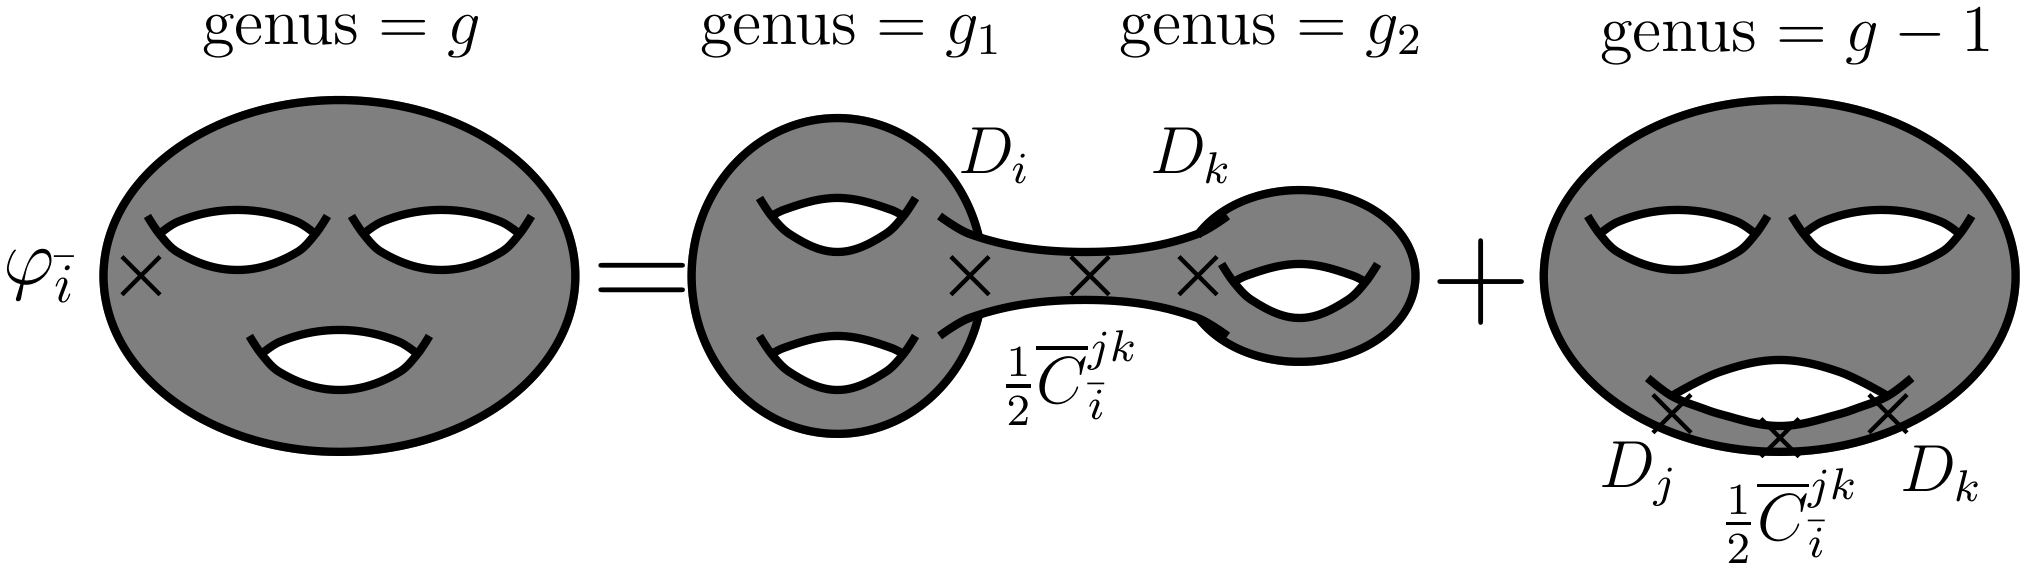
\includegraphics[width=0.95\linewidth]{figures/figure-1.png}
  \caption{全纯反常方程 (4.24) 的费曼图式图解：左侧为亏格 $g$ 的黎曼面，其上有算符
    $\phi_{\bar\imath}$ 的插入（以 $\times$ 标记）；右端为两类退化情形——中间是亏格 $g_1$ 与 $g_2$
    （$g_1+g_2=g$）的两部分经由一条细管相连，最右是亏格 $g-1$ 的黎曼面；$D_i,D_j,D_k$ 表示对相应
    模参数的协变导数，$\frac12\bar C^{jk}_{\bar\imath}$ 为相应的耦合因子。（原文第 31 页，式 (4.24)
    之后；原文未编号，此处编号为译者所加）}
  \label{fig:1}
\end{figure}

其中 $g>1$，并且
\begin{equation}
  \bar C^{ij}_{\bar k}=\bar C_{\bar\imath\bar\jmath\bar k}G^{i\bar\imath}G^{j\bar\jmath}e^{2K}\,,\qquad
  \bar C_{\bar\imath\bar\jmath\bar k}=\overline{C_{ijk}}\,.
  \tag{4.25}
  \label{eq:4.25}
\end{equation}
对 $g=1$，方程为
\begin{equation}
  \bar\partial_{\bar\imath}\mathcal{F}^{(1)}_j
  =\frac12C_{jkl}C^{kl}_{\bar\imath}
  +\Big(1-\frac{\chi}{24}\Big)G_{j\bar\imath}\,.
  \tag{4.26}
  \label{eq:4.26}
\end{equation}
% [原文疑误: 同 (4.11)，此处 C^{kl}_{\bar\imath} 疑漏上划线，应为 \bar C^{kl}_{\bar\imath}。照抄原文。]

% [Tutor Note: 易错点] 反常方程的归一化因子、$1/2$ 与有序求和、$\chi/24$ 修正、指标升降
\begin{yizhu}[易错点]
此处最易出错的是因子与求和约定：(i) (4.24) 的 $\frac12$ 与 $\sum_{g_1+g_2=g}$ 配套——求和遍历
有序对 $(g_1,g_2)$，故 $1/2$ 不可漏；第二项 $D_jD_k\mathcal{F}^{(g-1)}$ 不属于该求和。(ii) $g=1$ 时
(4.24) 的求和退化，须改用 (4.26)，其中 $\chi$ 是 Calabi--Yau 三维流形的 Euler 数，$(1-\chi/24)$ 是
$g=1$（单圈）反常方程的已知系数；$\frac12C_{jkl}C^{kl}_{\bar\imath}$ 的两个上标 $k,l$ 与 $C_{jkl}$
完全缩并，漏一个因子便破坏 $\bar\partial_{\bar\imath}\mathcal{F}^{(1)}_j$ 的 $(1,1)$ 型。
(iii) 指标升降要用 Zamolodchikov 度规的逆 $G^{i\bar\imath}$ 而非原度规 $g^{i\bar\imath}$：由
$g_{0\bar 0}=e^{-K}$ 与 (4.15) 得 $g^{i\bar\jmath}=e^{K}G^{i\bar\jmath}$；而 (4.25) 中的 $e^{2K}$ 是为
补足 $\bar C$ 的线丛权，不可与逆度规的 $e^{K}$ 因子混为一谈。(4.13) 的 $-i$ 与 (4.15) 的 $+i$ 也不可
互换。
\end{yizhu}

% ==== 原文 PDF 第 32 页 ====

\subsubsection*{以费曼图表示的解}

BCOV 在提出反常方程 \cite{ref19} 的同时，也提出了递推求解 $\mathcal{F}^{(g)}$ 的方法。其想法是对反常方程中
出现的反全纯导数作分部积分，直到得到如下形式的表达式
\[
  \partial_{\bar\imath}A=\partial_{\bar\imath}B\ \Rightarrow\ A=B+f(z)\,,
\]
其中 $f(z)$ 是全纯模糊性（holomorphic ambiguity）。为了在实践中做到这一点，他们首先注意到反全纯汤川
耦合可以局部地写为
\[
  \bar C_{\bar\imath\bar\jmath\bar k}=e^{-2K}D_iD_j\bar\partial_{\bar k}S\,,
\]
其中 $S$ 是 $\mathcal{L}^{-2}$ 的截面。还可以进一步引入一些对象 $S^{ij}$、$S^i$，它们分别是
$\mathcal{L}^{-2}\otimes\mathrm{Sym}^2(T^*\mathcal{M})$ 与 $\mathcal{L}^{-2}\otimes
T^*(\mathcal{M})$ 的截面，使得
\begin{equation}
  \bar\partial_{\bar\imath}S^{ij}=\bar C^{ij}_{\bar\imath}\,,\qquad
  \bar\partial_{\bar\imath}S^j=G_{i\bar\imath}S^{ij}\,,\qquad
  \bar\partial_{\bar\imath}S=G_{i\bar\imath}S^i\,.
  \tag{4.27}
  \label{eq:4.27}
\end{equation}
现在的做法是依次对反常方程作分部积分，首先写出
\begin{equation}
  \begin{aligned}
    &\bar\partial_{\bar\imath}\Big(\mathcal{F}^{(g)}
      -\frac12S^{jk}\Big(\sum_{g_1+g_2=g}D_j\mathcal{F}^{(g_1)}D_k\mathcal{F}^{(g_2)}
      +D_jD_k\mathcal{F}^{(g-1)}\Big)\Big)\\
    &\qquad=-\frac12S^{jk}\bar\partial_{\bar\imath}
      \Big(\sum_{g_1+g_2=g}D_j\mathcal{F}^{(g_1)}D_k\mathcal{F}^{(g_2)}
      +D_jD_k\mathcal{F}^{(g-1)}\Big)\,,
  \end{aligned}
  \tag{4.28}
  \label{eq:4.28}
\end{equation}
然后反复使用所得到的曲率表达式 $[\bar\partial_{\bar\imath},D_j]$（即 (4.11)）以及 $\tilde g<g$ 时
$\bar\partial_{\bar\imath}\mathcal{F}^{\tilde g}$ 的已知结果，即可得到所需结论。他们进一步指出，
如果把该系统视为比模空间 $\mathcal{M}$ 的维数多一个自由度的量子系统，则由此得到的表达式类似于费曼图：
其传播子为
\[
  K^{ij}=-S^{ij}\,,\qquad K^{i\phi}=-S^i\,,\qquad\text{以及}\qquad K^{\phi\phi}=-2S\,,
\]
而顶点由带插入的关联函数给出。此外，他们还给出了按费曼图展开的证明。

% [Tutor Note: 物理图像] 分部积分与费曼图递推的组合结构、全纯模糊性的地位
\begin{yizhu}[物理图像]
(4.28) 的关键是用 $\bar\partial_{\bar\imath}S^{ij}=\bar C^{ij}_{\bar\imath}$（(4.27)）把反常方程改写成
“左端只含 $\bar\partial_{\bar\imath}\mathcal{F}^{(g)}$ 与非全纯汤川耦合、右端只含较低亏格振幅的
$\bar\partial_{\bar\imath}$”的形式；反复使用 (4.11) 给出的 $[\bar\partial_{\bar\imath},D_j]$ 与已知的
$\bar\partial_{\bar\imath}\mathcal{F}^{\tilde g}$（$\tilde g<g$）即可逐级积分出 $\mathcal{F}^{(g)}$。
把 $S^{ij},S^i,S$ 视为传播子、把汤川耦合与带插入的关联函数视为顶点，则每一次分部积分相当于在图上接
一条内线或一个顶点，而图的亏格就是所计算的亏格——这正是“以费曼图表示的解”的含义；原文提到该系统比
$\mathcal{M}$ 多一个自由度，对应的就是 $S$ 那条带 $\phi$ 指标的传播子链。需注意递推只确定非全纯部分，
全纯模糊性 $f(z)$ 必须在每一步由边界条件固定（原文此处未展开，见 \cite{ref19} 及后文）。
\end{yizhu}

然而，这一做法的一个实际缺点是迭代次数增长极快，$\mathcal{F}^{(g)}$ 的表达会变得很长。另一方面，
反常方程所包含的递推信息在每一步都需要用边界条件来补充，以确定全纯模糊性。

% ============================================================
% 片段：s04b  对应原文 PDF 第 32--38 页
% 内容：§4.4 高亏格振幅的多项式结构；§4.5 使用多项式结构（4.5.1--4.5.3）；致谢
% 译者：t-s04b   审校状态：初稿
% 说明：原文 4.5.2、4.5.3 中的不编号斜体小标题（Genus 1、Higher genus boundary
%       conditions 等）在原文中为 \paragraph 级斜体标题，此处以斜体独立行复现。
% ============================================================

% ==== 原文 PDF 第 32 页（§4.4 起） ====

\subsection{高亏格振幅的多项式结构}
\label{sec:4.4}

\begin{keytakeaways}
  \begin{itemize}[leftmargin=1.4em,itemsep=2pt,topsep=2pt]
    \item \textbf{物理图像}：拓扑弦的高亏格自由能可解释为物理弦理论的某些振幅；完整的拓扑弦配分函数
          还被猜想编码了 4d BPS 态的信息 \cite{ref73}，因此自由能理应带有靶空间对偶群的自守形式结构。
    \item \textbf{数学工具}：特殊几何，具体说是出现在全纯反常方程右端的联络多重导数。Yamaguchi 与
          Yau 用 $A_p=G^{z\bar z}(z\partial_z)^pG_{z\bar z}$、$B_p=e^{K}(z\partial_z)^pe^{-K}$ 与全纯
          生成元 $X\sim1/\Delta$ 组成生成元环，并把它约化为 $A_1,B_1,B_2,B_3$ 与 $X$。
    \item \textbf{关键结论}：复结构形变空间为一维时，高亏格振幅是有限个生成元中次数为 $3g-3+n$ 的
          多项式 \cite{ref21}；任意维模空间的情形由生成元 $K_i,S^{ij},S^i,S$（分次 $1,1,2,3$）实现，式 (4.29)
          的换元使振幅不再依赖 $\tilde K_i$ \cite{ref22}。
    \item \textbf{技术核心}：反常方程在生成元的求导下封闭（式 (4.32)），故每一步递推只是把低亏格的
          已知量代数地组合起来；剩下的全纯模糊性由第~\ref{sec:4.5.2}~节的边界条件逐阶固定。
  \end{itemize}
\end{keytakeaways}

% [Tutor Note: 物理图像] 多项式结构的物理根源：非全纯部分由低亏格骨架唯一决定
\begin{yizhu}[物理图像]
“多项式结构”之所以可能，是因为反常方程右端只含有限几类量：汤川耦合 $C_{ijk}$、凯勒势 $K$ 及其
导数、以及联络 $\Gamma^l_{ij}$ 的若干组合。递推时，$\bar\partial_{\bar\imath}\mathcal{F}^{(g)}$
被这些“原子”乘上低亏格振幅的组合表示出来，因此 $\mathcal{F}^{(g)}$ 的非全纯依赖永远是有限个生成元
的多项式；新的物理信息只藏在全纯积分常数里。这正是“高亏格振幅由低亏格骨架决定”的精确表述，也解释
了为何振幅在对偶群下的模性足以用来确定反常方程的解 \cite{ref19}。
\end{yizhu}

拓扑弦的高亏格自由能可以解释为给出物理弦理论的某些振幅。\footnote{综述见文献 \cite{ref72}。} 完整的
拓扑弦配分函数被猜想也编码了 4d BPS 态的信息 \cite{ref73}。因此很自然地期望，%
% ==== 原文 PDF 第 33 页 ====
拓扑弦的自由能由靶空间对偶群的自守形式（automorphic forms）刻画。文献 \cite{ref19} 利用拓扑弦振幅的模性
（modularity）来确定反常方程的解。每当模群是 $\mathrm{SL}(2,\mathbb{Z})$ 或其子群时，振幅的模性
表现得最为明显。椭圆曲线的 Gromov--Witten 不变量的高亏格生成函数曾被写成多项式 \cite{ref74,ref75}，其多项式
生成元是近全纯模形式（almost holomorphic modular forms）环的元素 $E_2$、$E_4$ 与 $E_6$ \cite{ref76}。只要
$\mathrm{SL}(2,\mathbb{Z})$ 是模群的子群，这类生成元的多项式也会出现，例如见文献
\cite{ref77,ref78,ref79,ref80,ref28,ref81}。拓扑弦与近全纯模形式的关系在文献 \cite{ref23,ref82,ref24} 中得到进一步探讨。然而，
对于大多数 CY 流形的模空间及其单值群（monodromy group），相应的自守形式并不知道。结果表明，仅用
特殊几何就足以证明高亏格拓扑弦振幅的多项式结构 \cite{ref21,ref22}，下面将对此加以综述。

Yamaguchi 与 Yau 在 \cite{ref21} 中证明：对于镜像五次超曲面以及复结构形变空间为一维的相关几何，拓扑弦的
高亏格振幅可以表示为有限个生成元中次数为 $3g-3+n$ 的多项式，其中 $n$ 指插入算符的个数。作为多项式
的生成元，他们使用了特殊几何中的某些元素，也就是出现在全纯反常方程右端的那些量——联络的多重导数。
文献 \cite{ref21} 的非全纯生成元由
\[
  A_p = G^{z\bar z}(z\partial_z)^p G_{z\bar z},
  \qquad
  B_p = e^{K}(z\partial_z)^p e^{-K},
  \qquad p=1,2,3,\ldots
\]
给出。此外还使用了一个全纯生成元 $X\sim 1/\Delta$，其中 $\Delta$ 为判别式。下一步要证明生成元之间的
关系，使得无穷多个非全纯生成元可以约化为 $A_1$、$B_1$、$B_2$ 与 $B_3$。进一步，由全纯反常方程的
分析可以证明 \cite{ref21}：拓扑弦振幅中只出现生成元的特殊组合，因而非全纯生成元的数目又减少一个。

% [Tutor Note: 含糊点] “生成元之间的关系”与“特殊组合”两句跳过了 \cite{ref21} 的核心技术步骤
\begin{yizhu}[含糊点]
原文只说“证明生成元之间的关系”而把无穷多个 $A_p,B_p$ 约化为 $A_1,B_1,B_2,B_3$，又说“只出现特殊
组合”使数目再减一，但未写出这些关系式。就 \cite{ref21} 的构造而言，约化依赖于 $A_p,B_p$ 之间由特殊几何导出
的微分关系，以及反常方程中这些量只以特定组合出现这一事实；具体关系式原文未给。核对时应直接查文献
\cite{ref21} 的生成元关系式，不要试图由本讲义的叙述推出。
\end{yizhu}

将这一构造推广到模空间维数任意的 CY 流形，是在文献 \cite{ref22} 中给出的。\footnote{这一问题由 P. Mayr
在一份未发表的手稿中独立解决。} 下面将综述这一构造，以及为在递推的每一步求解全纯模糊性所需的边界
条件。

文献 \cite{ref22} 证明：关联函数 $\mathcal{F}^{(g)}_{i_1\cdots i_n}$ 是生成元 $K_i$、$S^{ij}$、$S^i$、$S$
中次数为 $3g-3+n$ 的多项式，这些生成元的分次（grading）分别取为 $1,1,2,3$。文献 \cite{ref22} 进一步证明，
通过如下生成元变换
\begin{equation}\tag{4.29}
\begin{aligned}
  \tilde S^{ij} &= S^{ij}, \\
  \tilde S^i &= S^i - S^{ij}K_j, \\
  % ==== 原文 PDF 第 34 页 ====
  \tilde S &= S - S^iK_i + \frac{1}{2}S^{ij}K_iK_j, \\
  \tilde K_i &= K_i,
\end{aligned}
\end{equation}
$\mathcal{F}^{(g)}$ 不依赖于 $\tilde K_i$，即 $\partial\mathcal{F}^{(g)}/\partial\tilde K_i=0$。
下文将去掉修改后生成元上的波浪号。

% [Tutor Note: 含糊点] (4.29) 中的换元与 (4.34) 中 $\partial/\partial K_j$ 项的基准问题
\begin{yizhu}[含糊点]
式 (4.29) 之后紧接着断言 $\partial\mathcal{F}^{(g)}/\partial\tilde K_i=0$，而式 (4.34) 右端却保留
$G_{\bar\imath j}\partial\mathcal{F}^{(g)}/\partial K_j$。这一点原文没有展开：它并未交代 (4.34)
写在未加波浪号还是已加波浪号的那一套生成元下，也未说明该断言的证明。阅读时只要记住 (4.29) 是一次
保持分次的生成元变换（$\tilde S$ 的表达式相当于把 $S$ 沿 $S^i$ 方向作平移 $K$ 后“配方”），
$K$ 的依赖被平移进 $\tilde S^i$ 与 $\tilde S$ 之中；(4.34) 则按原文形式照录，未作改写。核对时请以
文献 \cite{ref22} 的原始推导为准。
\end{yizhu}

证明的出发点是：把最先出现的非零关联函数用这些生成元表示。在亏格零，这些就是全纯三点耦合
$\mathcal{F}^{(0)}_{ijk}=C_{ijk}$。全纯反常方程 (4.24) 可以利用 (4.27) 积分，得到
\begin{equation}\tag{4.30}
\mathcal{F}^{(1)}_i
= \frac{1}{2}C_{ijk}S^{jk} + \left(1-\frac{\chi}{24}\right)K_i + f^{(1)}_i,
\end{equation}
其中 $f^{(1)}_i$ 为模糊性。由这一表达式可以看出，关联函数的非全纯性只来自生成元。此外，特殊几何关系
(4.11) 可以积分为
\begin{equation}\tag{4.31}
\Gamma^l_{ij} = \delta^l_i K_j + \delta^l_j K_i - C_{ijk}S^{kl} + s^l_{ij},
\end{equation}
其中 $s^l_{ij}$ 表示未被特殊几何关系固定的全纯函数；由此可以导出下列方程，它们表明承载非全纯性的
生成元在求导下封闭 \cite{ref22}。\footnote{这些方程是对式 (4.29) 中带波浪号的生成元写出的，可由文献 \cite{ref22}
中的方程直接得到。}
\begin{equation}\tag{4.32}
\begin{aligned}
  \partial_i S^{jk} &= C_{imn}S^{mj}S^{nk} + \delta^j_i S^k + \delta^k_i S^j
      - s^j_{im}S^{mk} - s^k_{im}S^{mj} + h_i^{jk}, \\
  \partial_i S^j &= C_{imn}S^{mj}S^n + 2\delta^j_i S
      - s^j_{im}S^m - h_{ik}S^{kj} + h^j_i, \\
  \partial_i S &= \frac{1}{2}C_{imn}S^m S^n - h_{ij}S^j + h_i, \\
  \partial_i K_j &= K_iK_j - C_{ijn}S^{mn}K_m + s^m_{ij}K_m - C_{ijk}S^k + h_{ij},
\end{aligned}
\end{equation}
其中 $h_i^{jk}$、$h_i^j$、$h_i$ 与 $h_{ij}$ 表示全纯函数。所有这些函数与式 (4.31) 中的函数并非彼此
独立。文献 \cite{ref26} 证明（另见 \cite{ref25}）：在此环中选取全纯函数的自由度归结为函数 $\mathcal{E}^{ij}$、
$\mathcal{E}^j$ 与 $\mathcal{E}$，它们可以加到多项式生成元上
\begin{equation}\tag{4.33}
\begin{aligned}
  \widehat{S}^{ij} &= S^{ij} + \mathcal{E}^{ij}, \\
  \widehat{S}^j &= S^j + \mathcal{E}^j, \\
  \widehat{S} &= S + \mathcal{E}.
\end{aligned}
\end{equation}
所有全纯量都相应地改变。

% [Tutor Note: 易错点] $S^{ij}$（生成元）与 $s^l_{ij}$（全纯系数）是两类完全不同的对象
\begin{yizhu}[易错点]
式 (4.31)--(4.33) 中大小写极易混淆：$S^{ij}$ 是非全纯的传播子型生成元，而 $s^l_{ij}$ 是用于重写联络
的全纯函数；同理 $\Gamma^l_{ij}$ 含非全纯部分，$\mathcal{E}^{ij}$、$\mathcal{E}^j$、$\mathcal{E}$ 则
纯全纯。核对时按“是否含反全纯指标”区分：$s$、$h$、$\mathcal{E}$ 都是全纯的待定函数，它们的选取对应
(4.33) 的自由度；而 $S^{ij},S^i,S$ 一旦被定义为生成元，其反全纯导数就由 (4.32) 唯一给出。
\end{yizhu}

% [Tutor Note: 易错点] 生成元的分次与多项式次数 $3g-3+n$ 的核算
\begin{yizhu}[易错点]
原文说生成元 $K_i,S^{ij},S^i,S$ 的分次（grading）依次为 $1,1,2,3$，注意 $S^{ij}$ 的分次也是 $1$，
并非 $2$。可用式 (4.30) 自检：$g=1$、$n=1$ 时总次数应为 $3g-3+n=1$，而式中 $C_{ijk}S^{jk}$ 与
$K_i$ 都恰为一次。若误把 $S^{ij}$ 记为二次，则后续所有“次数为 $3g-3+n$”的计数（以及 (4.37)、
(4.38) 的量纲）都会出错。
\end{yizhu}

现在，拓扑弦振幅满足的全纯反常方程中，$\bar\partial_{\bar\imath}$ 导数被替换为对多项式生成元的
导数 \cite{ref28,ref22}。
\begin{equation}\tag{4.34}
\bar\partial_{\bar\imath}\mathcal{F}^{(g)}
= \bar{C}^{jk}_{\bar\imath}\Bigl\{
  \frac{\partial\mathcal{F}^{(g)}}{\partial S^{jk}}
  - \frac{1}{2}\frac{\partial\mathcal{F}^{(g)}}{\partial S^k}K_j
  - \frac{1}{2}\frac{\partial\mathcal{F}^{(g)}}{\partial S^j}K_k
  + \frac{1}{2}\frac{\partial\mathcal{F}^{(g)}}{\partial S}K_jK_k \Bigr\}
+ G_{\bar\imath j}\frac{\partial\mathcal{F}^{(g)}}{\partial K_j}
\end{equation}
% ==== 原文 PDF 第 35 页 ====
\begin{equation}\tag{4.35}
\begin{aligned}
&= \frac{1}{2}\bar{C}^{jk}_{\bar\imath}\Bigl\{
  \Bigl(\partial_j\partial_k + (C_{jkm}S^{ml} - s^l_{jk})\partial_l
  + (4-2g)(h_{jk} - C_{jkl}S^l) \\
&\qquad + (3-2g)K_j\partial_k + (3-2g)K_k\partial_j
  + (4-2g)(3-2g)K_kK_j\Bigr)\mathcal{F}^{(g-1)} \\
&\quad + \sum_{h=1}^{g-1}\partial_j\mathcal{F}^{(g-h)}\partial_k\mathcal{F}^{(h)}
  + (2-2h)K_j\mathcal{F}^{(h)}\partial_k\mathcal{F}^{(g-h)}
  + (2-2g+2h)K_k\mathcal{F}^{(g-h)}\partial_j\mathcal{F}^{(h)} \\
&\qquad + K_jK_k(2-2h)(2-2g+2h)\mathcal{F}^{(h)}\mathcal{F}^{(g-h)}
  \Bigr\}.
\end{aligned}
\end{equation}

\subsection{使用多项式结构}
\label{sec:4.5}

\begin{keytakeaways}
  \begin{itemize}[leftmargin=1.4em,itemsep=2pt,topsep=2pt]
    \item \textbf{物理图像}：多项式结构把“解无穷多个亏格的反常方程”化归为“有限个待定系数的代数问题”：
          每个亏格的 $\mathcal{F}^{(g)}$ 写成生成元的多项式，系数是模参数的函数，再由边界条件逐步确定。
    \item \textbf{数学工具}：取局部坐标 $z_*$ 使 $C_{*ij}$ 可逆，由此从特殊几何关系反解出 $S^{ij}$
          （式 (4.36)）；再用闭合方程 (4.32) 逐次构造 $S^i$、$S$（式 (4.37)、(4.38)）。边界条件有三类：
          大复结构极限的常映射贡献 (4.42)、类锥形流形处的奇异结构 (4.43)，以及全纯模糊性的局部 ansatz
          (4.44)——后者的有限个系数由前两类条件固定。
    \item \textbf{关键结论}：生成元与 $s,h$ 的全纯规范选定后，高亏格振幅的全部模糊性化为
          $\Delta^{-(2g-2)}$ 乘一个低次多项式 $p(z)$ 的有限个系数；这些系数被 (4.42)、(4.43) 等边界
          条件线性地固定。
    \item \textbf{例}：五次超曲面在 $g=1$ 由 (4.46) 的 $n,\chi,s,r$ 完全确定（式 (4.47)）；$g=2$ 的
          (4.48) 给出多项式结构的一次显式检验。
  \end{itemize}
\end{keytakeaways}

% [Tutor Note: 物理图像] 4.5 节三步走：造生成元、给边界条件、在五次超曲面上验证
\begin{yizhu}[物理图像]
本节把上一小节的结论变成可执行的算法，分三步：(1) 构造生成元，即在模空间的局部坐标下把
$S^{ij},S^i,S$ 具体解出来（4.5.1）；(2) 给出边界条件，用大复结构极限、类锥形流形轨迹与全纯模糊性的
ansatz 固定每一步的积分常数（4.5.2）；(3) 在五次超曲面上显式执行到 $g=2$（4.5.3）。之所以能做第三
步，是因为多项式结构保证每个 $g$ 只有有限个未知系数，而边界条件恰好给出同样多的线性方程。
\end{yizhu}

\subsubsection{构造生成元}
\label{sec:4.5.1}

\begin{keytakeaways}
  \begin{itemize}[leftmargin=1.4em,itemsep=2pt,topsep=2pt]
    \item \textbf{物理图像}：$S^{ij}$、$S^i$、$S$ 就是反常方程右端那些非全纯数据的“积分”，在费曼图
          图像中充当传播子；构造生成元即选定一组传播子与全纯规范。
    \item \textbf{数学工具}：取局部坐标 $z_*$ 使 $C_{*ij}$ 可逆，从特殊几何关系 (4.31) 反解出 $S^{ij}$
          （式 (4.36)），再用闭合方程 (4.32) 逐次解出 $S^i$、$S$（式 (4.37)、(4.38)）。
    \item \textbf{关键结论}：一旦全纯函数 $s$、$h$ 按 (4.33) 的自由度选定，全部生成元就确定下来，
          且所有全纯函数都化为局部坐标 $z$ 的多项式或有理式——高亏格振幅的多项式结构由此落地。
  \end{itemize}
\end{keytakeaways}

多项式构造中生成元的构造方式已在文献 \cite{ref26} 中讨论。出发点是选取模空间上的一个局部坐标 $z_*$，使
$C_{*ij}$ 为可逆的 $n\times n$ 矩阵，从而把式 (4.31) 改写为
\begin{equation}\tag{4.36}
S^{ij} = \left(C_*^{-1}\right)^{ik}
\left(\delta^j_* K_k + \delta^j_k K_* - \Gamma^j_{*k} + s^j_{*k}\right),
\end{equation}
式 (4.33) 中的自由度可用来选定部分 $s^k_{ij}$ \cite{ref26}。其余生成元则利用方程 (4.32) 构造 \cite{ref26}：
\begin{equation}\tag{4.37}
S^i = \frac{1}{2}\left(\partial_i S^{ii} - C_{imn}S^{mi}S^{ni}
     + 2s^i_{im}S^{mi} - h_i^{ii}\right),
\end{equation}
\begin{equation}\tag{4.38}
S = \frac{1}{2}\left(\partial_i S^i - C_{imn}S^m S^{ni}
   + s^i_{im}S^m + h_{im}S^{mi} - h_i^i\right).
\end{equation}
在这两个式子中指标 $i$ 是固定的，即对该指标不求和。式 (4.33) 中给生成元添加全纯函数的自由度，同样
可用来对函数 $h_i^{ii}$、$h_i^i$ 作某种选择；其余函数由这一选择固定，并可由式 (4.32) 算出。

% [Tutor Note: 物理图像] $S^{ij},S^i,S$ 就是 §4.3 费曼图图像中的传播子
\begin{yizhu}[物理图像]
生成元的物理意义直接来自第 4.3 节的费曼图图像：$S^{ij}$、$S^i$、$S$ 分别是 $K^{ij}=-S^{ij}$、
$K^{i\phi}=-S^i$、$K^{\phi\phi}=-2S$ 这些传播子，而 $C_{*ij}$ 可逆的局部坐标保证了可以“解出”传播子。
所谓“构造生成元”，就是选定一组传播子与全纯规范，使得建立反常方程所需的全部全纯函数都成为局部坐标
$z$ 的有理式乃至多项式——这正是高亏格振幅能写成多项式的技术前提。
\end{yizhu}

% [Tutor Note: 易错点] (4.36) 的固定指标 $*$ 与矩阵求逆的缩并方式
\begin{yizhu}[易错点]
式 (4.36) 的指标结构极易写错：$C_{*ij}$ 可逆，$(C_*^{-1})^{ik}$ 与 $C_{*kl}$ 在 $k$ 上缩并，故
$S^{ij}$ 的两个自由指标是 $i,j$；$\Gamma^j_{*k}$ 与 $s^j_{*k}$ 的固定指标 $*$ 不是求和指标。另一个
常见错误是把 $\delta^j_* K_k$ 与 $\delta^j_k K_*$ 互换——由 (4.31) 反解可知，前者的 $K$ 带下标 $k$
（与 $C$ 的第二指标缩并），后者带固定指标 $*$。建议用 $n=1$ 的最简情形逐项验证一次。
\end{yizhu}

% [Tutor Note: 易错点] (4.37)、(4.38) 中“指标 i 固定”的约定
\begin{yizhu}[易错点]
式 (4.37)、(4.38) 下方特意声明“指标 $i$ 固定，不求和”，这是全文最容易漏掉的约定：$S^{ii}$ 中的
$i$ 不求和，而 $C_{imn}S^{mi}S^{ni}$ 中 $m,n$ 求和。这两式是把闭合方程 (4.32) 沿某一固定方向（对
五次超曲面即唯一的 $z$ 方向）解出 $S^i$、$S$ 的结果，因此只能在该方向上有意义；若误按爱因斯坦约定
对 $i$ 求和，两式都会变成平凡恒等式而失去内容。
\end{yizhu}

\subsubsection{边界条件}
\label{sec:4.5.2}

\begin{keytakeaways}
  \begin{itemize}[leftmargin=1.4em,itemsep=2pt,topsep=2pt]
    \item \textbf{物理图像}：边界条件把 $\mathcal{F}^{(g)}$ 钉在模空间的边界上：大复结构极限处是
          常映射的拓扑贡献，类锥形流形轨迹处是额外无质量超多重态造成的奇异结构。
    \item \textbf{数学工具}：$g=1$ 的显式积分 (4.39)；常映射公式 (4.42)；锥形流形处的主导奇异与
          “间隙” (4.43)；全纯模糊性的局部 ansatz (4.44)。
    \item \textbf{关键结论}：$g=1$ 的系数 $s_i$、$r_a$ 被 (4.40)、(4.41) 完全固定；$g\ge2$ 时每个亏格
          只剩下 $p(z_i)$ 的有限个系数，由 (4.42)、(4.43) 给出的线性方程唯一确定。
  \end{itemize}
\end{keytakeaways}

% 原文此处为不编号的斜体小标题（\paragraph 级）
\medskip
\noindent\emph{亏格 1}\par

亏格 1 的全纯反常方程 (4.26) 可以积分给出
\begin{equation}\tag{4.39}
\mathcal{F}^{(1)}
= \frac{1}{2}\left(3+n-\frac{\chi}{12}\right)K
+ \frac{1}{2}\log\det G^{-1}
+ \sum_i s_i\log z_i
+ \sum_a r_a\log\Delta_a ,
\end{equation}
其中 $i=1,\ldots,n=h^{1,1}(Z)=h^{2,1}(Z^*)$，而 $a$ 遍历判别式的各个分支。系数 $s_i$ 与 $r_a$ 由
$\mathcal{F}^{(1)}$ 的主导奇异行为固定：对代数坐标 $z_i$，该行为由文献 \cite{ref19} 给出为
\begin{equation}\tag{4.40}
\mathcal{F}^{(1)} \sim -\frac{1}{24}\sum_i \log z_i \int_Z c_2 J_i ,
\end{equation}
% ==== 原文 PDF 第 36 页 ====
而对与锥形流形（conifold）奇点相对应的判别式 $\Delta$，主导行为由
\begin{equation}\tag{4.41}
\mathcal{F}^{(1)} \sim -\frac{1}{12}\log\Delta .
\end{equation}
给出。

% [Tutor Note: 易错点] (4.39) 的系数与 $\chi$ 的约定
\begin{yizhu}[易错点]
式 (4.39) 中 $K$ 的系数是 $\frac{1}{2}\left(3+n-\frac{\chi}{12}\right)$，注意这里的 $\chi$ 是靶空间
的欧拉示性数，$\chi=2\left(h^{1,1}-h^{2,1}\right)$，符号约定不同文献可能差一个整体符号；$n$ 同时
等于 $h^{1,1}(Z)$ 与 $h^{2,1}(Z^*)$。$\frac{1}{2}\log\det G^{-1}$ 项来自 $g=1$ 反常方程积分时的
Zamolodchikov 度规贡献，不要与 (4.42) 中的 $\frac{\chi}{2}$ 因子混淆。
\end{yizhu}

% [Tutor Note: 物理图像] (4.40) 与 (4.41) 如何固定 $s_i$、$r_a$
\begin{yizhu}[物理图像]
式 (4.40) 与 (4.41) 是固定 (4.39) 中待定系数的两条边界信息：前者给出 $z_i\to0$（大复结构/大体积）
处的对数发散，其系数由第二陈类 $c_2$ 沿曲线的积分给出；后者给出锥形流形轨迹 $\Delta=0$ 处的
$-\frac{1}{12}\log\Delta$ 发散。两者合起来给出了 $s_i$ 与 $r_a$ 的全部约束，因此 $g=1$ 的振幅可以被
完全确定——这正是 4.5.3 中 (4.46) 取值的来源。
\end{yizhu}

% 原文此处为不编号的斜体小标题（\paragraph 级）
\medskip
\noindent\emph{高亏格边界条件}\par

重构完整拓扑弦振幅所需的全纯模糊性，可以通过对 $\mathcal{F}^{(g)}$ 在模空间边界上施加各种边界条件
来固定。

% 原文此处为不编号的斜体小标题（\paragraph 级）
\medskip
\noindent\emph{大复结构极限}\par

$\mathcal{F}^{(g)}$ 在该点（它镜像于大体积极限）的主导行为已在文献 \cite{ref18,ref19,ref83,ref13,ref84,ref14} 中
算出。特别地，常映射的贡献为
\begin{equation}\tag{4.42}
\mathcal{F}^{(g)}\big|_{q_a=0}
= (-1)^g\frac{\chi}{2}\,
  \frac{|B_{2g}B_{2g-2}|}{2g(2g-2)(2g-2)!},
\qquad g>1,
\end{equation}
其中 $q_a$ 表示该点处指数化的镜像映射。

% [Tutor Note: 物理图像] 常映射贡献是 $F^{(g)}$ 中唯一与模无关的部分
\begin{yizhu}[物理图像]
式 (4.42) 是常映射的贡献：世界面不携带任何手征插入、整体映射到靶空间一点。它只依赖靶空间的
拓扑（$\chi$）与亏格，是固定亏格下唯一与模参数无关的项，因此给出 $\mathcal{F}^{(g)}$ 在大复结构
极限处的一个“锚点”。$B_{2g}$ 与 $B_{2g-2}$ 的出现来自常数映射下对亏格 $g$ 世界面模空间的积分
（所有世界面都映到同一点，只剩下模空间上的特征类积分），其组合
$|B_{2g}B_{2g-2}|/\left(2g(2g-2)(2g-2)!\right)$ 也是 $g$ 很大时 $\mathcal{F}^{(g)}$ 增长的主要来源，
这使该边界条件对高亏格递推非常强。
\end{yizhu}

% 原文此处为不编号的斜体小标题（\paragraph 级）
\medskip
\noindent\emph{类锥形流形轨迹}\par

配分函数 $\mathcal{F}^{(g)}$ 在锥形流形轨迹处的主导奇异行为已在文献 \cite{ref18,ref19,ref85,ref86,ref13,ref14} 中
确定：
\begin{equation}\tag{4.43}
\mathcal{F}^{(g)}(t_c)
= b\,\frac{B_{2g}}{2g(2g-2)\,t_c^{2g-2}} + O(t_c^0),
\qquad g>1 .
\end{equation}
这里 $t_c\sim\Delta^{1/m}$ 是判别式轨迹 $\Delta=0$ 处的平坦坐标。对于锥形流形奇点，$b=1$、$m=1$。
特别地，(4.43) 中的主导奇异性以及次主导奇异项的缺失，来自文献 \cite{ref13,ref14} 的 Schwinger 圈计算，该计算
给出时空理论中额外无质量超多重态（hypermultiplet）的效应 \cite{ref87}。这种奇异结构以及次主导奇异项的
“间隙”（gap），也在对偶矩阵模型中观察到 \cite{ref88}，并首先被文献 \cite{ref89,ref90} 用来固定高亏格的全纯模糊性。
文献 \cite{ref13,ref14} 的时空推导并不限于锥形流形情形，也适用于 $m>1$ 的奇点，后者在时空中给出由额外无质量
矢量多重态与超多重态组成的不同谱。Schwinger 圈积分的系数是对粒子自旋的加权求迹 \cite{ref87,ref86}，由此预言
主导奇异项的系数为 $b=n_H-n_V$。前因子（prefactor）$b$ 在 $m>1$ 情形下的出现，已在文献 \cite{ref26} 中就
局部 $\mathbb{F}_2$ 的情形讨论过（另见 \cite{ref91}）。

% [Tutor Note: 易错点] (4.43) 的“间隙”性质给出多个线性条件
\begin{yizhu}[易错点]
式 (4.43) 有两个易错点。其一，$t_c\sim\Delta^{1/m}$ 中的 $m$ 不一定为 $1$；$m>1$ 时前因子为
$b=n_H-n_V$，需要用局部模型的谱重新计算，而不是简单取 $b=1$。其二，“次主导奇异项的缺失”是指
在主导项 $t_c^{2-2g}$ 之后，所有更奇异的项（如 $t_c^{1-2g}$ 等）都缺席（gap）；$O(t_c^0)$ 表示允许
常数项与正规项，并非“全部为零”。正因为有这个间隙，一次边界条件能同时钉死 $p(z_i)$ 中的一批系数；
把它误读成“所有更高项为零”会导致系数超定、方程组无解。
\end{yizhu}

% ==== 原文 PDF 第 37 页 ====

% 原文此处为不编号的斜体小标题（\paragraph 级）
\medskip
\noindent\emph{全纯模糊性}\par

$\mathcal{F}^{(g)}$ 的奇异行为通过全纯模糊性的如下局部 ansatz 加以考虑：
\begin{equation}\tag{4.44}
\mathrm{hol.ambiguity} \sim \frac{p(\tilde z_i)}{\Delta^{(2g-2)}} ,
\end{equation}
其中 $p(\tilde z_i)$ 先验地是奇点附近局部坐标 $\tilde z_i$ 的级数。然而，把各奇点处的局部信息与
具有有限单值性的边界除子拼接起来，可知分子 $p(z_i)$ 一般只是 $z_i$ 的低次多项式。这里 $z_i$ 表示
以大复结构为中心的自然坐标，$z_i=0\ \forall i$。$p(z_i)$ 中有限个系数受 (4.43) 约束。高亏格振幅的
多项式结构结合这些边界条件，足以在局部 CY 流形上微扰地求解拓扑弦理论（例如见文献 \cite{ref92,ref26}），也使
得在紧致 CY 流形上求解高亏格振幅成为可能 \cite{ref90,ref91,ref28}。

% [Tutor Note: 含糊点] (4.44) 中 $\tilde z_i$ 与 $z_i$ 的记号切换
\begin{yizhu}[含糊点]
式 (4.44) 及其上一句用局部坐标 $\tilde z_i$ 写 ansatz，紧接着的讨论却改用大复结构坐标 $z_i$，原文
未明说这是同一个对象的两种坐标。可这样理解：$p$ 先在奇点附近的局部坐标中是级数，拼接（patching）
到全局并把各边界除子的信息纳入后，其分子在自然坐标 $z_i$ 下成为低次多项式；$z_i$ 正是 (4.47) 中
$P=\Delta^{-1}$ 所用的坐标。核对 (4.44) 与 (4.47)、(4.48) 时，须把 $p$ 理解为 $z$ 的多项式。
\end{yizhu}

\subsubsection{例：五次超曲面}
\label{sec:4.5.3}

\begin{keytakeaways}
  \begin{itemize}[leftmargin=1.4em,itemsep=2pt,topsep=2pt]
    \item \textbf{物理图像}：五次超曲面是最简单的单参数例子（$h^{1,1}=1$、$\chi=-200$），用来演示
          多项式结构如何变成逐亏格的显式计算。
    \item \textbf{数学工具}：全纯函数的指标乘除 $z$ 约定、按文献 \cite{ref25} 选取的 $s$、$h$ 值 (4.45)、
          亏格 1 的边界数据 (4.46)、以及由此固定的 $z\partial_z\mathcal{F}^{(1)}$ (4.47)。
    \item \textbf{关键结论}：$g=1$ 与 $g=2$ 的振幅都被完全固定，其中 $g=2$ 的显式结果 (4.48) 是多项式
          结构可用性的直接检验；用同一套办法可以走到很高亏格 \cite{ref90}。
    \item \textbf{可核对性}：$P=\Delta^{-1}$ 视为 $0$ 次，则 (4.48) 中每一项的总次数都不超过
          $3g-3=3$，这是检验抄录与理解是否正确的快捷判据。
  \end{itemize}
\end{keytakeaways}

% 原文此处为不编号的斜体小标题（\paragraph 级）
\medskip
\noindent\emph{生成元的选取}\par

多项式生成元的选取方式是固定的：使式 (4.31)、(4.32) 中出现的全纯函数都是 $z$ 的有理表达式，其中
$z$ 是模空间大复结构片中的坐标。对于这些全纯函数，下列上下指标分别乘以、除以 $z$：
\[
  A^j_i \to \frac{z_i}{z_j}A^j_i .
\]
采用这一约定后，多项式构造框架中出现的所有全纯函数都可以用局部坐标的多项式表示（见文献
\cite{ref21,ref22,ref25}）。这些全纯函数按文献 \cite{ref25} 选取为
\begin{equation}\tag{4.45}
s^z_{zz} = -\frac{8}{5},
\qquad
h^{zz}_z = \frac{1}{25},
\qquad
h^z_z = -\frac{1}{125},
\qquad
h_z = \frac{2}{3125},
\qquad
h_{zz} = \frac{2}{25},
\end{equation}

% [Tutor Note: 易错点] 指标乘除 $z$ 的约定与 (4.45) 的归一化
\begin{yizhu}[易错点]
$A^j_i\to(z_i/z_j)A^j_i$ 这一约定不是装饰：它把不同权重的全纯函数按 $z$ 的幂次归一，使得 (4.45) 中
的常数成为纯数字。若漏掉该约定，或改用另一套 $z$ 的归一化（例如把大复结构坐标乘以常数），(4.45) 的
数值就会改变。核对时请同时对照文献 \cite{ref25} 的坐标定义与 (4.47) 中 $P=\Delta^{-1}$ 的定义；这三处必须
用同一个 $z$。
\end{yizhu}

% 原文此处为不编号的斜体小标题（\paragraph 级）
\medskip
\noindent\emph{亏格 1}\par

利用亏格 1 的边界条件，可以如下固定关于 $\mathcal{F}^1$ 的方程 (4.39)：
\begin{equation}\tag{4.46}
n = 1, \qquad \chi = -200, \qquad s = -\frac{31}{12}, \qquad r = -\frac{1}{12},
\end{equation}
而起始的多项式表达式被固定为（其中 $P=\Delta^{-1}$）：
\begin{equation}\tag{4.47}
z\partial_z\mathcal{F}^{(1)}
= \frac{1}{60}\left(-112 + 560K_z + 5P(1+30S^{zz})\right).
\end{equation}

% [Tutor Note: 物理图像] (4.46) 的 $\chi=-200$ 与五次超曲面的霍奇数
\begin{yizhu}[物理图像]
式 (4.46) 的数值都可以独立核对：五次超曲面有 $h^{1,1}=1$、$h^{2,1}=101$，故
$\chi = 2(h^{1,1}-h^{2,1}) = 2(1-101) = -200$，$n=h^{1,1}=1$；而 $s=-\frac{31}{12}$、
$r=-\frac{1}{12}$ 分别由 (4.40) 在 $z\to0$ 的主导行为与 (4.41) 在 $\Delta\to0$ 的主导行为确定。
也就是说，在 (4.39) 的形式下 $g=1$ 的振幅不再含由 $s_i$、$r_a$ 表示的自由参数——它们已被边界条件
完全固定。
\end{yizhu}

% [Tutor Note: 易错点] (4.47) 中 $P$ 不是带分次的生成元
\begin{yizhu}[易错点]
式 (4.47) 与 (4.48) 中的 $P=\Delta^{-1}$ 是 $z$ 的全纯函数，不是 $K_i,S^{ij},S^i,S$ 那类带分次的
生成元；在次数核算中应把它按 $0$ 次处理。这解释了为何 (4.48) 中 $P^2$ 乘以三次项后总次数仍为
$3g-3=3$。另一个易错点是 (4.47) 左边是 $z\partial_z\mathcal{F}^{(1)}$ 而非 $\mathcal{F}^{(1)}$ 本身，
这是为了配合大复结构坐标下的多项式表示；抄录时注意 $P$ 项是 $5P(1+30S^{zz})$，括号内的 $1$ 不要
漏掉。
\end{yizhu}

% ==== 原文 PDF 第 38 页 ====

% 原文此处为不编号的斜体小标题（\paragraph 级）
\medskip
\noindent\emph{高亏格}\par

利用多项式形式 (4.34)、(4.35) 的全纯反常方程以及边界条件，可以固定高亏格振幅。例如在亏格 2、取上述
生成元时，得到
\begin{equation}\tag{4.48}
\begin{aligned}
\mathcal{F}^{(2)}
&= \frac{1}{36000}\Bigl(
  5P^2\left(37500(S^{zz})^3 + 6000(S^{zz})^2 + 325S^{zz} + 6\right) \\
&\qquad - P\left(25000S^z(30S^{zz}+1) + 150000(S^{zz})^2 + 4400S^{zz} - 23\right) \\
&\qquad + 16\left(175000S + 35000S^z + 3500S^{zz} - 39\right)\Bigr).
\end{aligned}
\end{equation}

% [Tutor Note: 物理图像] 用 Ref.\cite{ref21} 生成元加边界条件把五次解到高亏格的逻辑
\begin{yizhu}[物理图像]
(4.48) 是整套算法的样板：先用上面构造的生成元把 $\mathcal{F}^{(2)}$ 的非全纯部分由反常方程定出，
剩下的全纯模糊性按 (4.44) 型 ansatz 只有有限个系数；再用 (4.42) 的常映射项与 (4.43) 的间隙条件逐项
比较，恰好得到与未知系数个数相同的线性方程，解出的就是 (4.48) 中的那些数字（$36000$、$37500$、
$6000$、$325$、$25000$、$150000$、$4400$、$175000$、$35000$、$3500$、$39$ 等）。文献 \cite{ref90} 正是用
文献 \cite{ref21} 的多项式生成元、前面综述的边界条件，再加文献 \cite{ref93} 的不变量计数技巧，把五次超曲面解到了
很高的亏格。
\end{yizhu}

% [Tutor Note: 易错点] (4.48) 的逐项核对清单
\begin{yizhu}[易错点]
抄录 (4.48) 时建议按结构而非按行核对：整体是 $\frac{1}{36000}\left(5P^2A - PB + 16C\right)$，其中
$A=37500(S^{zz})^3+6000(S^{zz})^2+325S^{zz}+6$（三次到零次），
$B=25000S^z(30S^{zz}+1)+150000(S^{zz})^2+4400S^{zz}-23$（三次到零次），
$C=175000S+35000S^z+3500S^{zz}-39$（三次到零次）。三处最易出错：$B$ 中 $30S^{zz}+1$ 的括号范围、
$B$ 末项是 $-23$ 而非 $+23$、$C$ 末项是 $-39$；此外 $16$ 乘在整个 $C$ 上，不要漏乘。
\end{yizhu}

% ---------------------------------------------------------------------------
\section*{致谢}
\addcontentsline{toc}{section}{致谢}
% ---------------------------------------------------------------------------

我要感谢清华大学数学科学中心（Mathematical Sciences Center, Tsinghua University）与
Shing-Tung Yau 教授的盛情接待，以及邀请我作这些讲座。我还要感谢 Michael Hecht、Albrecht Klemm、
Dominique Länge、Peter Mayr、Emanuel Scheidegger、Shing-Tung Yau 与 Jie Zhou，就本讲义所涵盖的
某些课题及相关问题所作的讨论与合作。此外，我要感谢 Emanuel Scheidegger 与 Jie Zhou 对书稿的评论。
本工作由 DFG fellowship AL 1407/1-1 资助。

% [Tutor Note: 含糊点] 致谢中的外文姓名与资助编号照录
\begin{yizhu}[含糊点]
致谢中的人名按原文保留拉丁字母。Dominique Länge 的 “ä” 是德语变音，用 XeLaTeX 直接以 UTF-8 写入
即可，不要写成 “Lange”。资助编号 “AL 1407/1-1” 是德国研究基金会（DFG）的 fellowship 编号，属
专名，照抄不译。另外，原文的 “Prof. Shing-Tung Yau” 在两句感谢中重复出现，译文照原文保留这一重复。
\end{yizhu}

% ---------------------------------------------------------------------------
% 术语建议（供 Lead 统一时参考，未在正文中混用）：
%   automorphic forms = 自守形式；almost holomorphic modular forms = 近全纯模形式；
%   grading = 分次；hol.ambiguity = 全纯模糊性（原文用缩写，正文照录）。
% 版式说明：4.5.2、4.5.3、致谢中的不编号斜体小标题（Genus 1、The large complex
%   structure limit 等）原文为 \paragraph 级斜体标题，本片段用“斜体独立行”复现，
%   未新增编号层级；若全书统一改用 \paragraph* 或 \subsubsection*，可直接替换。
% ---------------------------------------------------------------------------

% ============================================================
% 片段：s05  参考文献（References）
% 对应原文 PDF 第 38--44 页（第 38 页 "References" 起，至第 44 页条目 [93] 止）
% 内容：文献 [1]--[93]，共 93 条，编号与原文严格一一对应
% 译者：t-refs   审校状态：初稿
% ============================================================

\section*{参考文献}
\addcontentsline{toc}{section}{参考文献}

% 说明（不改 main.tex）：main.tex 导言区已令 \refname=“参考文献”，而 article 类的
% thebibliography 环境会在列表前自动再排一个同名 \section* 标题。为避免正文出现两个
% “参考文献”，下面在一层 \begingroup...\endgroup 内把 \section 临时改为吞掉两个参数的
% 空宏，使环境自带的那个标题不排版；分组结束即自动恢复，不影响其他片段。
\begingroup
\renewcommand{\section}[2]{}%

\begin{thebibliography}{99}

% ==== 原文 PDF 第 38 页 ====

\bibitem{ref1}
N. Seiberg and E. Witten, ``Electric - magnetic duality, monopole condensation, and
confinement in $N=2$ supersymmetric Yang-Mills theory,'' \textit{Nucl.Phys.} \textbf{B426}
(1994) 19--52, \texttt{arXiv:hep-th/9407087 [hep-th]}.

\bibitem{ref2}
A. Klemm, W. Lerche, P. Mayr, C. Vafa, and N. P. Warner, ``Selfdual strings and $N=2$
supersymmetric field theory,'' \textit{Nucl.Phys.} \textbf{B477} (1996) 746--766,
\texttt{arXiv:hep-th/9604034 [hep-th]}.

\bibitem{ref3}
W. Lerche, ``Introduction to Seiberg-Witten theory and its stringy origin,''
\textit{Nucl.Phys.Proc.Suppl.} \textbf{55B} (1997) 83--117,
\texttt{arXiv:hep-th/9611190 [hep-th]}.

\bibitem{ref4}
L. J. Dixon, ``Some world-sheet properties of superstring compactifications, on orbifolds
and otherwise,'' in \textit{Superstrings, unified theories and cosmology 1987 (Trieste,
1987)}, vol. 4 of \textit{ICTP Ser. Theoret. Phys.}, pp. 67--126. World Sci. Publ.,
Teaneck, NJ, 1988.

\bibitem{ref5}
W. Lerche, C. Vafa, and N. P. Warner, ``Chiral Rings in $N=2$ Superconformal Theories,''
\textit{Nucl.Phys.} \textbf{B324} (1989) 427.

% ==== 原文 PDF 第 39 页 ====

\bibitem{ref6}
E. Witten, ``Mirror manifolds and topological field theory,''
\texttt{arXiv:hep-th/9112056 [hep-th]}.

\bibitem{ref7}
S.-T. Yau, ed., \textit{Mirror symmetry. I}, vol. 9 of \textit{AMS/IP Studies in Advanced
Mathematics}. American Mathematical Society, Providence, RI, 1998. Revised reprint of it
Essays on mirror manifolds [Internat. Press, Hong Kong, 1992; MR1191418 (94b:32001)].

\bibitem{ref8}
D. A. Cox and S. Katz, \textit{Mirror symmetry and algebraic geometry}, vol. 68 of
\textit{Mathematical Surveys and Monographs}. American Mathematical Society, Providence,
RI, 1999.

\bibitem{ref9}
K. Hori, S. Katz, A. Klemm, R. Pandharipande, R. Thomas, C. Vafa, R. Vakil, and E. Zaslow,
\textit{Mirror symmetry}, vol. 1 of \textit{Clay Mathematics Monographs}. American
Mathematical Society, Providence, RI, 2003. With a preface by Vafa.

\bibitem{ref10}
P. S. Aspinwall, T. Bridgeland, A. Craw, M. R. Douglas, M. Gross, A. Kapustin, G. W. Moore,
G. Segal, B. Szendr\H{o}i, and P. M. H. Wilson, \textit{Dirichlet branes and mirror
symmetry}, vol. 4 of \textit{Clay Mathematics Monographs}. American Mathematical Society,
Providence, RI, 2009.

\bibitem{ref11}
B. R. Greene and M. Plesser, ``Duality in Calabi-Yau Moduli Space,'' \textit{Nucl.Phys.}
\textbf{B338} (1990) 15--37.

\bibitem{ref12}
P. Candelas, X. C. De La Ossa, P. S. Green, and L. Parkes, ``A Pair of Calabi-Yau manifolds
as an exactly soluble superconformal theory,'' \textit{Nucl.Phys.} \textbf{B359} (1991)
21--74.

\bibitem{ref13}
R. Gopakumar and C. Vafa, ``$M$ theory and topological strings. 1.,''
\texttt{arXiv:hep-th/9809187 [hep-th]}.

\bibitem{ref14}
R. Gopakumar and C. Vafa, ``$M$ theory and topological strings. 2.,''
\texttt{arXiv:hep-th/9812127 [hep-th]}.

\bibitem{ref15}
S. H. Katz, A. Klemm, and C. Vafa, ``Geometric engineering of quantum field theories,''
\textit{Nucl.Phys.} \textbf{B497} (1997) 173--195,
\texttt{arXiv:hep-th/9609239 [hep-th]}.

\bibitem{ref16}
S. Katz, P. Mayr, and C. Vafa, ``Mirror symmetry and exact solution of 4-D $N=2$ gauge
theories: 1.,'' \textit{Adv.Theor.Math.Phys.} \textbf{1} (1998) 53--114,
\texttt{arXiv:hep-th/9706110 [hep-th]}.

\bibitem{ref17}
P. Mayr, ``Geometric construction of $N=2$ gauge theories,'' \textit{Fortsch.Phys.}
\textbf{47} (1999) 39--63, \texttt{arXiv:hep-th/9807096 [hep-th]}.

\bibitem{ref18}
M. Bershadsky, S. Cecotti, H. Ooguri, and C. Vafa, ``Holomorphic anomalies in topological
field theories,'' \textit{Nucl.Phys.} \textbf{B405} (1993) 279--304,
\texttt{arXiv:hep-th/9302103 [hep-th]}.

\bibitem{ref19}
M. Bershadsky, S. Cecotti, H. Ooguri, and C. Vafa, ``Kodaira-Spencer theory of gravity and
exact results for quantum string amplitudes,'' \textit{Commun.Math.Phys.} \textbf{165}
(1994) 311--428, \texttt{arXiv:hep-th/9309140 [hep-th]}.

\bibitem{ref20}
E. Witten, ``Quantum background independence in string theory,''
\texttt{arXiv:hep-th/9306122 [hep-th]}.

% ==== 原文 PDF 第 40 页 ====

\bibitem{ref21}
S. Yamaguchi and S.-T. Yau, ``Topological string partition functions as polynomials,''
\textit{JHEP} \textbf{0407} (2004) 047, \texttt{arXiv:hep-th/0406078 [hep-th]}.

\bibitem{ref22}
M. Alim and J. D. L\"ange, ``Polynomial Structure of the (Open) Topological String
Partition Function,'' \textit{JHEP} \textbf{0710} (2007) 045,
\texttt{arXiv:0708.2886 [hep-th]}.

\bibitem{ref23}
M. Aganagic, V. Bouchard, and A. Klemm, ``Topological Strings and (Almost) Modular Forms,''
\textit{Commun.Math.Phys.} \textbf{277} (2008) 771--819,
\texttt{arXiv:hep-th/0607100 [hep-th]}.

\bibitem{ref24}
T. W. Grimm, A. Klemm, M. Marino, and M. Weiss, ``Direct Integration of the Topological
String,'' \textit{JHEP} \textbf{0708} (2007) 058,
\texttt{arXiv:hep-th/0702187 [HEP-TH]}.

\bibitem{ref25}
S. Hosono, ``BCOV ring and holomorphic anomaly equation,''
\texttt{arXiv:0810.4795 [math.AG]}.

\bibitem{ref26}
M. Alim, J. D. L\"ange, and P. Mayr, ``Global Properties of Topological String Amplitudes
and Orbifold Invariants,'' \textit{JHEP} \textbf{1003} (2010) 113,
\texttt{arXiv:0809.4253 [hep-th]}.

\bibitem{ref27}
M. Alim, \textit{Mirror symmetry, toric branes and topological string amplitudes as
polynomials}. PhD Thesis. Ludwig-Maximilians-University Library, Munich, 2009.
\url{http://edoc.ub.uni-muenchen.de/10341/}.

\bibitem{ref28}
M. Alim and E. Scheidegger, ``Topological Strings on Elliptic Fibrations,''
\texttt{arXiv:1205.1784 [hep-th]}.

\bibitem{ref29}
B. R. Greene, ``String theory on Calabi-Yau manifolds,''
\texttt{arXiv:hep-th/9702155 [hep-th]}.

\bibitem{ref30}
N. Warner, ``$N=2$ supersymmetric integrable models and topological field theories,''
\texttt{arXiv:hep-th/9301088 [hep-th]}.

\bibitem{ref31}
P. S. Aspinwall, ``D-branes on Calabi-Yau manifolds,''
\texttt{arXiv:hep-th/0403166 [hep-th]}.

\bibitem{ref32}
P. Fre and P. Soriani, ``The $N=2$ wonderland: From Calabi-Yau manifolds to topological
field theories,''. Singapore, Singapore: World Scientific (1995) 468 p.

\bibitem{ref33}
R. Dijkgraaf, H. Verlinde, and E. Verlinde, ``Notes on topological string theory and 2D
quantum gravity,'' in \textit{String theory and quantum gravity (Trieste, 1990)},
pp. 91--156. World Sci. Publ., River Edge, NJ, 1991.

\bibitem{ref34}
J. Walcher, ``Extended holomorphic anomaly and loop amplitudes in open topological
string,'' \textit{Nucl.Phys.} \textbf{B817} (2009) 167--207,
\texttt{arXiv:0705.4098 [hep-th]}.

\bibitem{ref35}
E. Witten, ``Topological Sigma Models,'' \textit{Commun.Math.Phys.} \textbf{118} (1988) 411.

\bibitem{ref36}
M. Vonk, ``A Mini-course on topological strings,''
\texttt{arXiv:hep-th/0504147 [hep-th]}.

\bibitem{ref37}
M. Marino, ``Chern-Simons theory and topological strings,'' \textit{Rev.Mod.Phys.}
\textbf{77} (2005) 675--720, \texttt{arXiv:hep-th/0406005 [hep-th]}.

\bibitem{ref38}
M. Marino, ``Les Houches lectures on matrix models and topological strings,''
\texttt{arXiv:hep-th/0410165 [hep-th]}.

% ==== 原文 PDF 第 41 页 ====

\bibitem{ref39}
A. Neitzke and C. Vafa, ``Topological strings and their physical applications,''
\texttt{arXiv:hep-th/0410178 [hep-th]}.

\bibitem{ref40}
M. Mari\~no, \textit{Chern-Simons theory, matrix models and topological strings}, vol. 131
of \textit{International Series of Monographs on Physics}. The Clarendon Press Oxford
University Press, Oxford, 2005.
\url{http://dx.doi.org/10.1093/acprof:oso/9780198568490.001.0001}.

\bibitem{ref41}
B. Pioline, ``Lectures on black holes, topological strings and quantum attractors (2.0),''
\textit{Lect.Notes Phys.} \textbf{755} (2008) 283--373.

\bibitem{ref42}
E. Witten, ``Phases of $N=2$ theories in two-dimensions,'' \textit{Nucl.Phys.}
\textbf{B403} (1993) 159--222, \texttt{arXiv:hep-th/9301042 [hep-th]}.

\bibitem{ref43}
P. S. Aspinwall, B. R. Greene, and D. R. Morrison, ``Calabi-Yau moduli space, mirror
manifolds and space-time topology change in string theory,'' \textit{Nucl.Phys.}
\textbf{B416} (1994) 414--480, \texttt{arXiv:hep-th/9309097 [hep-th]}.

\bibitem{ref44}
P. S. Aspinwall, B. R. Greene, and D. R. Morrison, ``Measuring small distances in $N=2$
sigma models,'' \textit{Nucl.Phys.} \textbf{B420} (1994) 184--242,
\texttt{arXiv:hep-th/9311042 [hep-th]}.

\bibitem{ref45}
C. Voisin, \textit{Mirror symmetry}, vol. 1 of \textit{SMF/AMS Texts and Monographs}.
American Mathematical Society, Providence, RI, 1999. Translated from the 1996 French
original by Roger Cooke.

\bibitem{ref46}
V. V. Batyrev and D. van Straten, ``Generalized hypergeometric functions and rational
curves on Calabi-Yau complete intersections in toric varieties,''
\textit{Commun.Math.Phys.} \textbf{168} (1995) 493--534,
\texttt{arXiv:alg-geom/9307010 [alg-geom]}.

\bibitem{ref47}
V. Bouchard and R. Cavalieri, ``On the mathematics and physics of high genus invariants of
[C**3 / Z(3)],'' \textit{Adv.Theor.Math.Phys.} \textbf{13} (2009) 695--719,
\texttt{arXiv:0709.3805 [math.AG]}.

\bibitem{ref48}
M. Gross, ``Calabi-Yau manifolds and mirror symmetry,'' in \textit{Calabi-Yau manifolds and
related geometries (Nordfjordeid, 2001)}, Universitext, pp. 69--159. Springer, Berlin,
2003. \url{http://dx.doi.org/10.1007/978-3-642-19004-9_2}.

\bibitem{ref49}
C. Voisin, \textit{Hodge theory and complex algebraic geometry. I}, vol. 76 of
\textit{Cambridge Studies in Advanced Mathematics}. Cambridge University Press, Cambridge,
2002. \url{http://dx.doi.org/10.1017/CBO9780511615344}. Translated from the French original
by Leila Schneps.

\bibitem{ref50}
W. Lerche, D. Smit, and N. Warner, ``Differential equations for periods and flat
coordinates in two-dimensional topological matter theories,'' \textit{Nucl.Phys.}
\textbf{B372} (1992) 87--112, \texttt{arXiv:hep-th/9108013 [hep-th]}.

\bibitem{ref51}
A. Ceresole, R. D'Auria, S. Ferrara, W. Lerche, J. Louis, and T. Regge, ``Picard-Fuchs
equations, special geometry and target space duality,''. Contribution to second volume of
`Essays on Mirror Manifolds'.

\bibitem{ref52}
B. de Wit and A. Van Proeyen, ``Potentials and Symmetries of General Gauged $N=2$
Supergravity: Yang-Mills Models,'' \textit{Nucl.Phys.} \textbf{B245} (1984) 89.

% ==== 原文 PDF 第 42 页 ====

\bibitem{ref53}
E. Cremmer, C. Kounnas, A. Van Proeyen, J. Derendinger, S. Ferrara, \textit{et al.},
``Vector Multiplets Coupled to $N=2$ Supergravity: SuperHiggs Effect, Flat Potentials and
Geometric Structure,'' \textit{Nucl.Phys.} \textbf{B250} (1985) 385.

\bibitem{ref54}
B. de Wit, P. Lauwers, and A. Van Proeyen, ``Lagrangians of $N=2$ Supergravity - Matter
Systems,'' \textit{Nucl.Phys.} \textbf{B255} (1985) 569.

\bibitem{ref55}
P. Candelas and X. de la Ossa, ``Moduli Space of Calabi-Yau Manifolds,'' \textit{Nucl.Phys.}
\textbf{B355} (1991) 455--481.

\bibitem{ref56}
A. Strominger, ``Special Geometry,'' \textit{Commun.Math.Phys.} \textbf{133} (1990)
163--180.

\bibitem{ref57}
S. Ferrara and J. Louis, ``Flat holomorphic connections and Picard-Fuchs identities from
$N=2$ supergravity,'' \textit{Phys.Lett.} \textbf{B278} (1992) 240--245,
\texttt{arXiv:hep-th/9112049 [hep-th]}.

\bibitem{ref58}
A. Ceresole, R. D'Auria, S. Ferrara, W. Lerche, and J. Louis, ``Picard-Fuchs equations and
special geometry,'' \textit{Int.J.Mod.Phys.} \textbf{A8} (1993) 79--114,
\texttt{arXiv:hep-th/9204035 [hep-th]}.

\bibitem{ref59}
D. S. Freed, ``Special K\"ahler manifolds,'' \textit{Comm. Math. Phys.} \textbf{203}
no. 1, (1999) 31--52. \url{http://dx.doi.org/10.1007/s002200050604}.

\bibitem{ref60}
S. Hosono, B. Lian, and S.-T. Yau, ``GKZ generalized hypergeometric systems in mirror
symmetry of Calabi-Yau hypersurfaces,'' \textit{Commun.Math.Phys.} \textbf{182} (1996)
535--578, \texttt{arXiv:alg-geom/9511001 [alg-geom]}.

\bibitem{ref61}
S. Hosono and B. Lian, ``GKZ hypergeometric systems and applications to mirror symmetry,''
\texttt{arXiv:hep-th/9602147 [hep-th]}.

\bibitem{ref62}
M. Noguchi, ``Mirror symmetry of Calabi-Yau manifolds and flat coordinates,''
\textit{Int.J.Mod.Phys.} \textbf{A12} (1997) 4973--4996,
\texttt{arXiv:hep-th/9609163 [hep-th]}.

\bibitem{ref63}
T. Masuda and H. Suzuki, ``Prepotentials, bilinear forms on periods and enhanced gauge
symmetries in Type II strings,'' \textit{Int.J.Mod.Phys.} \textbf{A14} (1999) 1177--1204,
\texttt{arXiv:hep-th/9807062 [hep-th]}.

\bibitem{ref64}
A. Klemm, ``Topological string theory on Calabi-Yau threefolds,'' \textit{PoS}
\textbf{RTN2005} (2005) 002.

\bibitem{ref65}
V. V. Batyrev, ``Dual Polyhedra and Mirror Symmetry for Calabi-Yau Hypersurfaces in Toric
Varieties,'' \texttt{arXiv:alg-geom/9310003 [alg-geom]}.

\bibitem{ref66}
S. Hosono, A. Klemm, S. Theisen, and S.-T. Yau, ``Mirror symmetry, mirror map and
applications to Calabi-Yau hypersurfaces,'' \textit{Commun.Math.Phys.} \textbf{167} (1995)
301--350, \texttt{arXiv:hep-th/9308122 [hep-th]}.

\bibitem{ref67}
K. Hori and C. Vafa, ``Mirror symmetry,'' \texttt{arXiv:hep-th/0002222 [hep-th]}.

\bibitem{ref68}
I. M. Gel'fand, A. V. Zelevinski\u{\i}, and M. M. Kapranov, ``Hypergeometric functions and
toric varieties,'' \textit{Funktsional. Anal. i Prilozhen.} \textbf{23} no. 2, (1989)
12--26. \url{http://dx.doi.org/10.1007/BF01078777}.

% ==== 原文 PDF 第 43 页 ====

\bibitem{ref69}
P. S. Aspinwall, ``The Moduli space of $N=2$ superconformal field theories,''
\texttt{arXiv:hep-th/9412115 [hep-th]}.

\bibitem{ref70}
S. Cecotti and C. Vafa, ``Topological antitopological fusion,'' \textit{Nucl.Phys.}
\textbf{B367} (1991) 359--461.

\bibitem{ref71}
A. Ceresole, R. D'Auria, and S. Ferrara, ``The Symplectic structure of $N=2$ supergravity
and its central extension,'' \textit{Nucl.Phys.Proc.Suppl.} \textbf{46} (1996) 67--74,
\texttt{arXiv:hep-th/9509160 [hep-th]}.

\bibitem{ref72}
I. Antoniadis and S. Hohenegger, ``Topological amplitudes and physical couplings in string
theory,'' \textit{Nucl.Phys.Proc.Suppl.} \textbf{171} (2007) 176--195,
\texttt{arXiv:hep-th/0701290 [HEP-TH]}.

\bibitem{ref73}
H. Ooguri, A. Strominger, and C. Vafa, ``Black hole attractors and the topological
string,'' \textit{Phys.Rev.} \textbf{D70} (2004) 106007,
\texttt{arXiv:hep-th/0405146 [hep-th]}.

\bibitem{ref74}
R. E. Rudd, ``The String partition function for QCD on the torus,''
\texttt{arXiv:hep-th/9407176 [hep-th]}.

\bibitem{ref75}
R. Dijkgraaf, ``Mirror symmetry and elliptic curves,'' in \textit{The moduli space of curves
(Texel Island, 1994)}, vol. 129 of \textit{Progr. Math.}, pp. 149--163. Birkh\"auser Boston,
Boston, MA, 1995.

\bibitem{ref76}
M. Kaneko and D. Zagier, ``A generalized Jacobi theta function and quasimodular forms,''
in \textit{The moduli space of curves (Texel Island, 1994)}, vol. 129 of \textit{Progr.
Math.}, pp. 165--172. Birkh\"auser Boston, Boston, MA, 1995.

\bibitem{ref77}
J. Minahan, D. Nemeschansky, C. Vafa, and N. Warner, ``$E$ strings and $N=4$ topological
Yang-Mills theories,'' \textit{Nucl.Phys.} \textbf{B527} (1998) 581--623,
\texttt{arXiv:hep-th/9802168 [hep-th]}.

\bibitem{ref78}
S. Hosono, M. Saito, and A. Takahashi, ``Holomorphic anomaly equation and BPS state
counting of rational elliptic surface,'' \textit{Adv.Theor.Math.Phys.} \textbf{3} (1999)
177--208, \texttt{arXiv:hep-th/9901151 [hep-th]}.

\bibitem{ref79}
S. Hosono, ``Counting BPS states via holomorphic anomaly equations,'' \textit{Fields
Inst.Commun.} (2002) 57--86, \texttt{arXiv:hep-th/0206206 [hep-th]}.

\bibitem{ref80}
A. Klemm, M. Kreuzer, E. Riegler, and E. Scheidegger, ``Topological string amplitudes,
complete intersection Calabi-Yau spaces and threshold corrections,'' \textit{JHEP}
\textbf{0505} (2005) 023, \texttt{arXiv:hep-th/0410018 [hep-th]}.

\bibitem{ref81}
A. Klemm, J. Manschot, and T. Wotschke, ``Quantum geometry of elliptic Calabi-Yau
manifolds,'' \texttt{arXiv:1205.1795 [hep-th]}.

\bibitem{ref82}
M. Gunaydin, A. Neitzke, and B. Pioline, ``Topological wave functions and heat equations,''
\textit{JHEP} \textbf{0612} (2006) 070, \texttt{arXiv:hep-th/0607200 [hep-th]}.

\bibitem{ref83}
M. Marino and G. W. Moore, ``Counting higher genus curves in a Calabi-Yau manifold,''
\textit{Nucl.Phys.} \textbf{B543} (1999) 592--614,
\texttt{arXiv:hep-th/9808131 [hep-th]}.

% ==== 原文 PDF 第 44 页 ====

\bibitem{ref84}
C. Faber and R. Pandharipande, ``Hodge integrals and Gromov-Witten theory,''
\textit{Inventiones Mathematicae} \textbf{139} (1999) 173--199,
\texttt{arXiv:98101173 [math.AG]}.

\bibitem{ref85}
D. Ghoshal and C. Vafa, ``$C=1$ string as the topological theory of the conifold,''
\textit{Nucl.Phys.} \textbf{B453} (1995) 121--128,
\texttt{arXiv:hep-th/9506122 [hep-th]}.

\bibitem{ref86}
I. Antoniadis, E. Gava, K. Narain, and T. Taylor, ``$N=2$ type II heterotic duality and
higher derivative $F$ terms,'' \textit{Nucl.Phys.} \textbf{B455} (1995) 109--130,
\texttt{arXiv:hep-th/9507115 [hep-th]}.

\bibitem{ref87}
C. Vafa, ``A Stringy test of the fate of the conifold,'' \textit{Nucl.Phys.} \textbf{B447}
(1995) 252--260, \texttt{arXiv:hep-th/9505023 [hep-th]}.

\bibitem{ref88}
M. Aganagic, A. Klemm, M. Marino, and C. Vafa, ``Matrix model as a mirror of Chern-Simons
theory,'' \textit{JHEP} \textbf{0402} (2004) 010, \texttt{arXiv:hep-th/0211098 [hep-th]}.

\bibitem{ref89}
M.-x. Huang and A. Klemm, ``Holomorphic Anomaly in Gauge Theories and Matrix Models,''
\textit{JHEP} \textbf{0709} (2007) 054, \texttt{arXiv:hep-th/0605195 [hep-th]}.

\bibitem{ref90}
M.-x. Huang, A. Klemm, and S. Quackenbush, ``Topological string theory on compact
Calabi-Yau: Modularity and boundary conditions,'' \textit{Lect.Notes Phys.} \textbf{757}
(2009) 45--102, \texttt{arXiv:hep-th/0612125 [hep-th]}.

\bibitem{ref91}
B. Haghighat and A. Klemm, ``Solving the Topological String on $K3$ Fibrations,''
\textit{JHEP} \textbf{1001} (2010) 009, \texttt{arXiv:0908.0336 [hep-th]}. With an appendix
by Sheldon Katz.

\bibitem{ref92}
B. Haghighat, A. Klemm, and M. Rauch, ``Integrability of the holomorphic anomaly
equations,'' \textit{JHEP} \textbf{0810} (2008) 097,
\texttt{arXiv:0809.1674 [hep-th]}.

\bibitem{ref93}
S. H. Katz, A. Klemm, and C. Vafa, ``$M$ theory, topological strings and spinning black
holes,'' \textit{Adv.Theor.Math.Phys.} \textbf{3} (1999) 1445--1537,
\texttt{arXiv:hep-th/9910181 [hep-th]}.

\end{thebibliography}
\endgroup


\end{document}
